\documentclass[10pt, oneside]{article} % The default font size and one-sided printing (no margin offsets)

\usepackage[spanish]{babel}
\usepackage{subfig}
\usepackage{titlesec}
\usepackage{array}
\usepackage{graphicx}
\usepackage{float}
\newcolumntype{L}[1]{>{\raggedright\let\newline\\\arraybackslash\hspace{0pt}}m{#1}}
\newcolumntype{C}[1]{>{\centering\let\newline\\\arraybackslash\hspace{0pt}}m{#1}}
\newcolumntype{R}[1]{>{\raggedleft\let\newline\\\arraybackslash\hspace{0pt}}m{#1}}

\begin{document}
 
\section{CuZr a distintas temperaturas}

%
%	Compresion
%

\subsection{Compresion}

\begin{figure}[H]
\centering
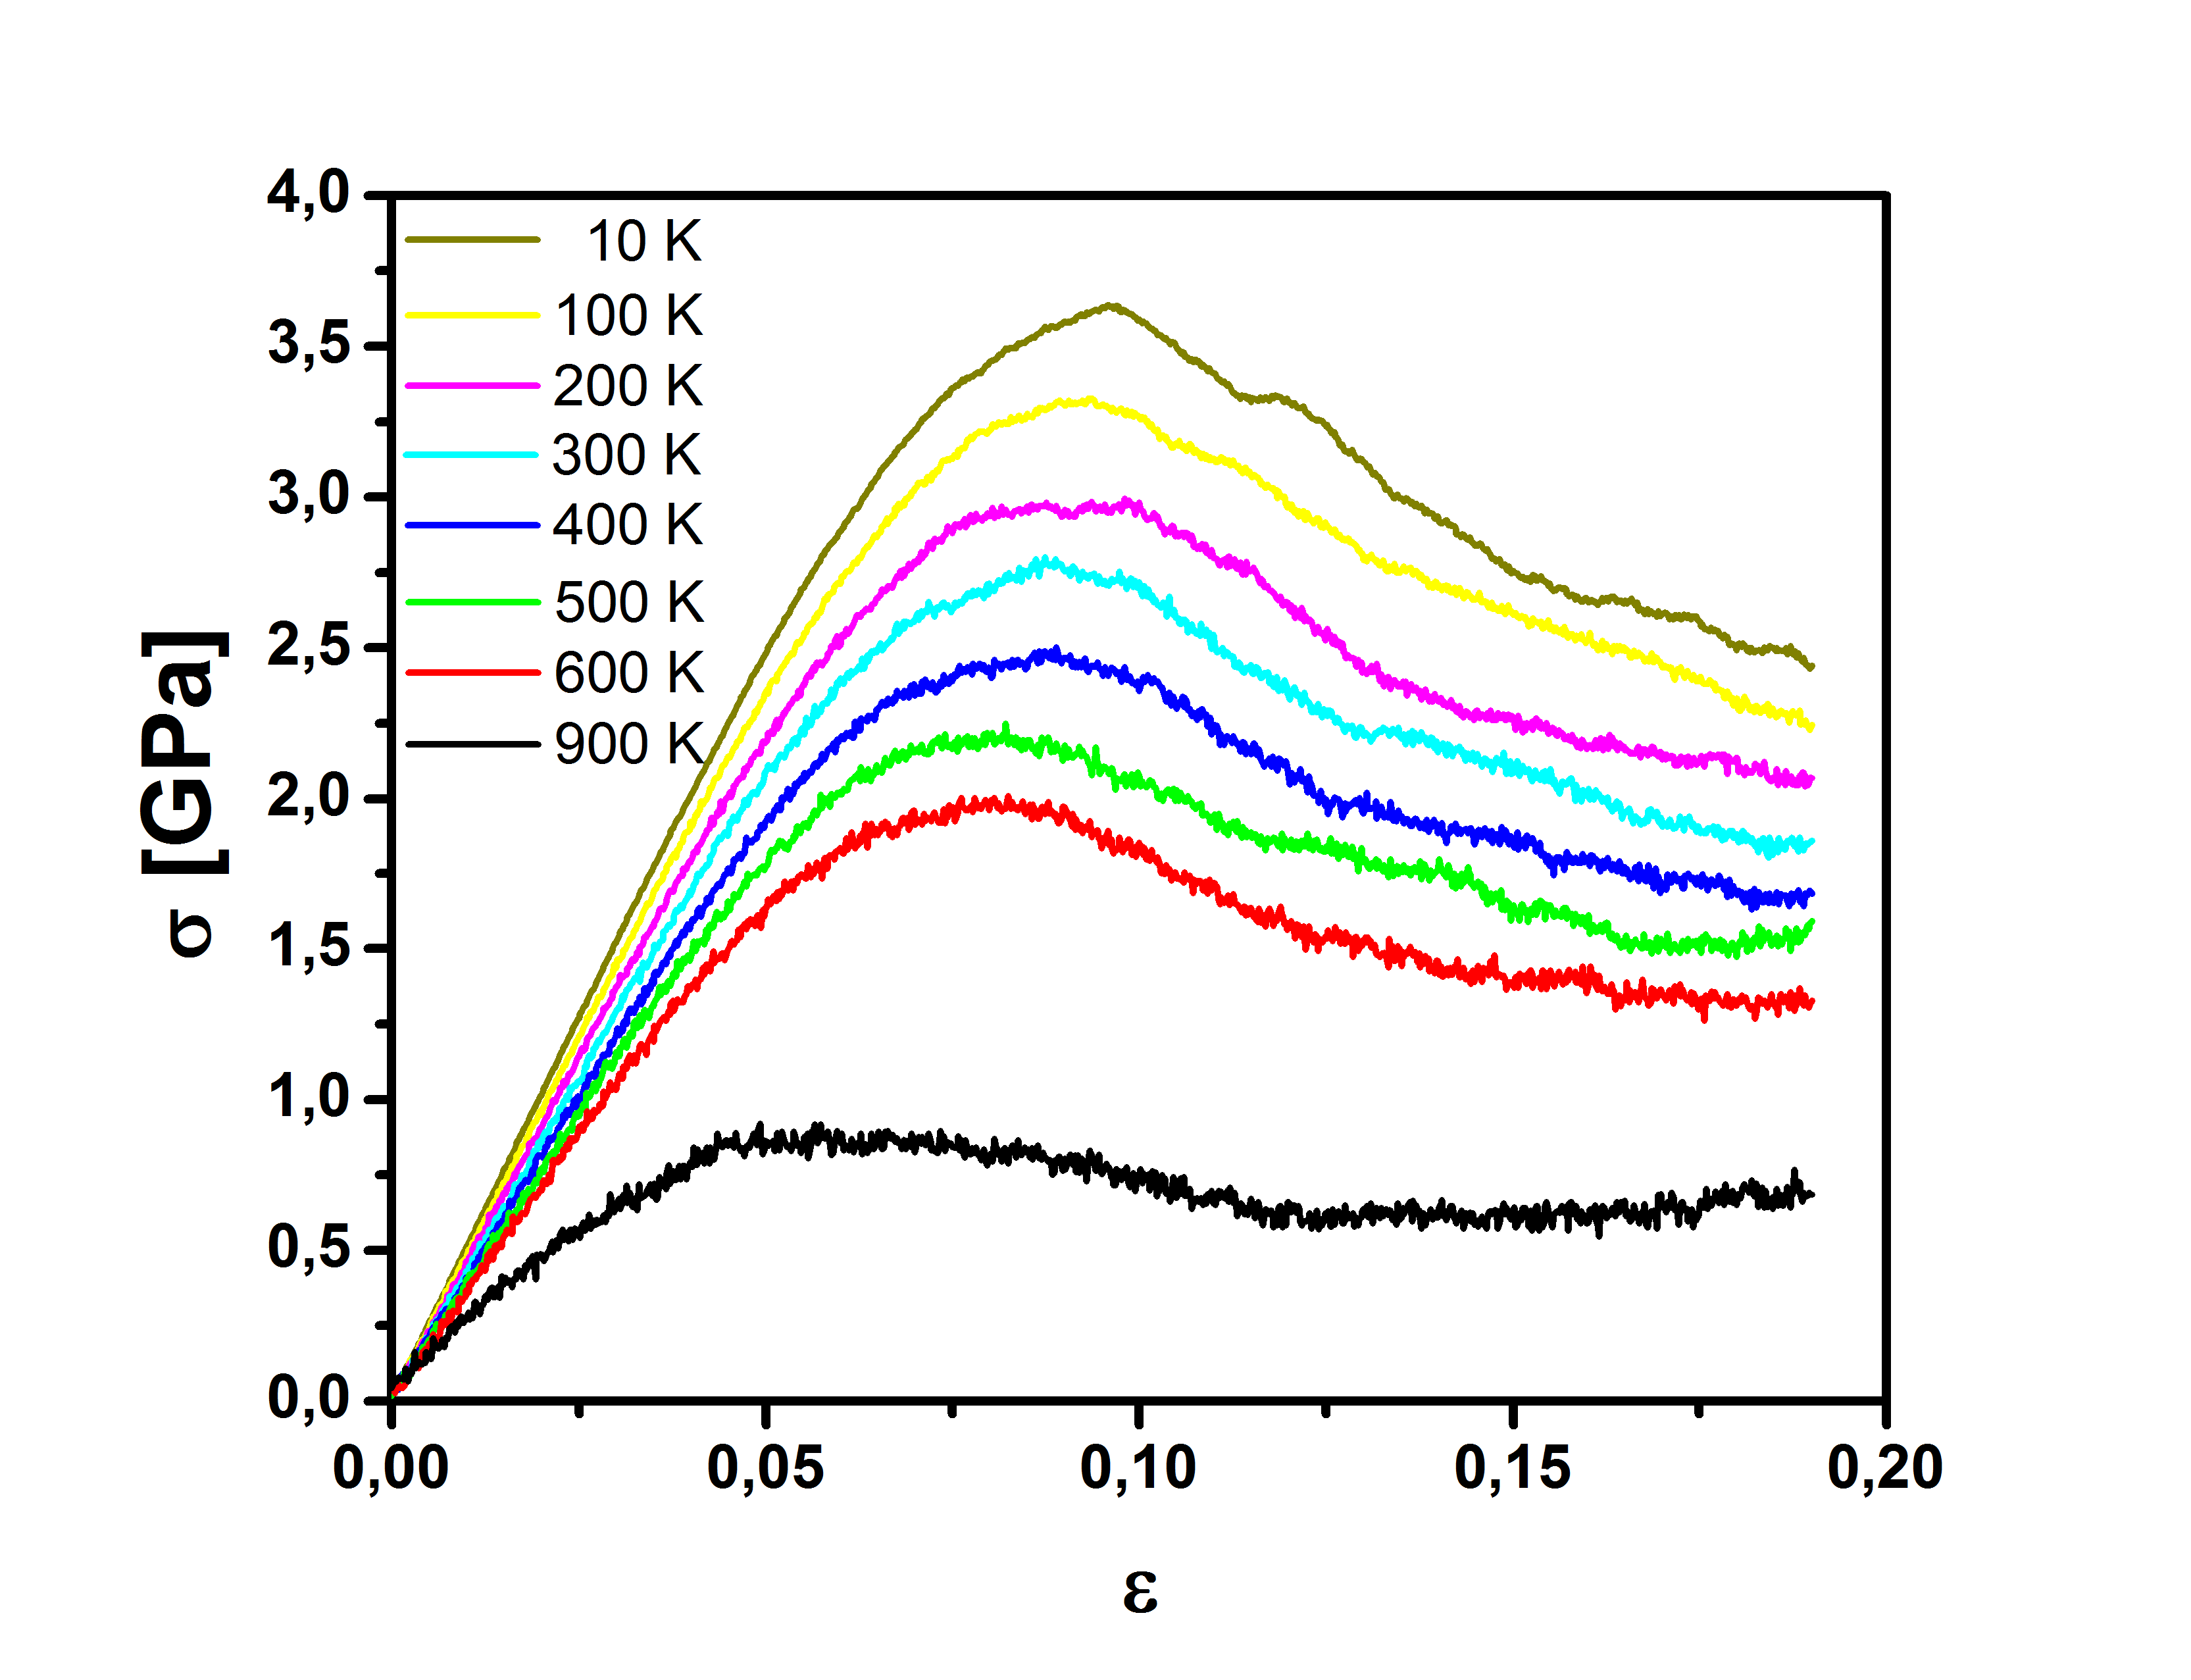
\includegraphics[width=8cm]{Figures/stress_strain_COMP.png}
\caption{Von Mises vs. strain}
\end{figure}

\begin{figure}[H]
\centering
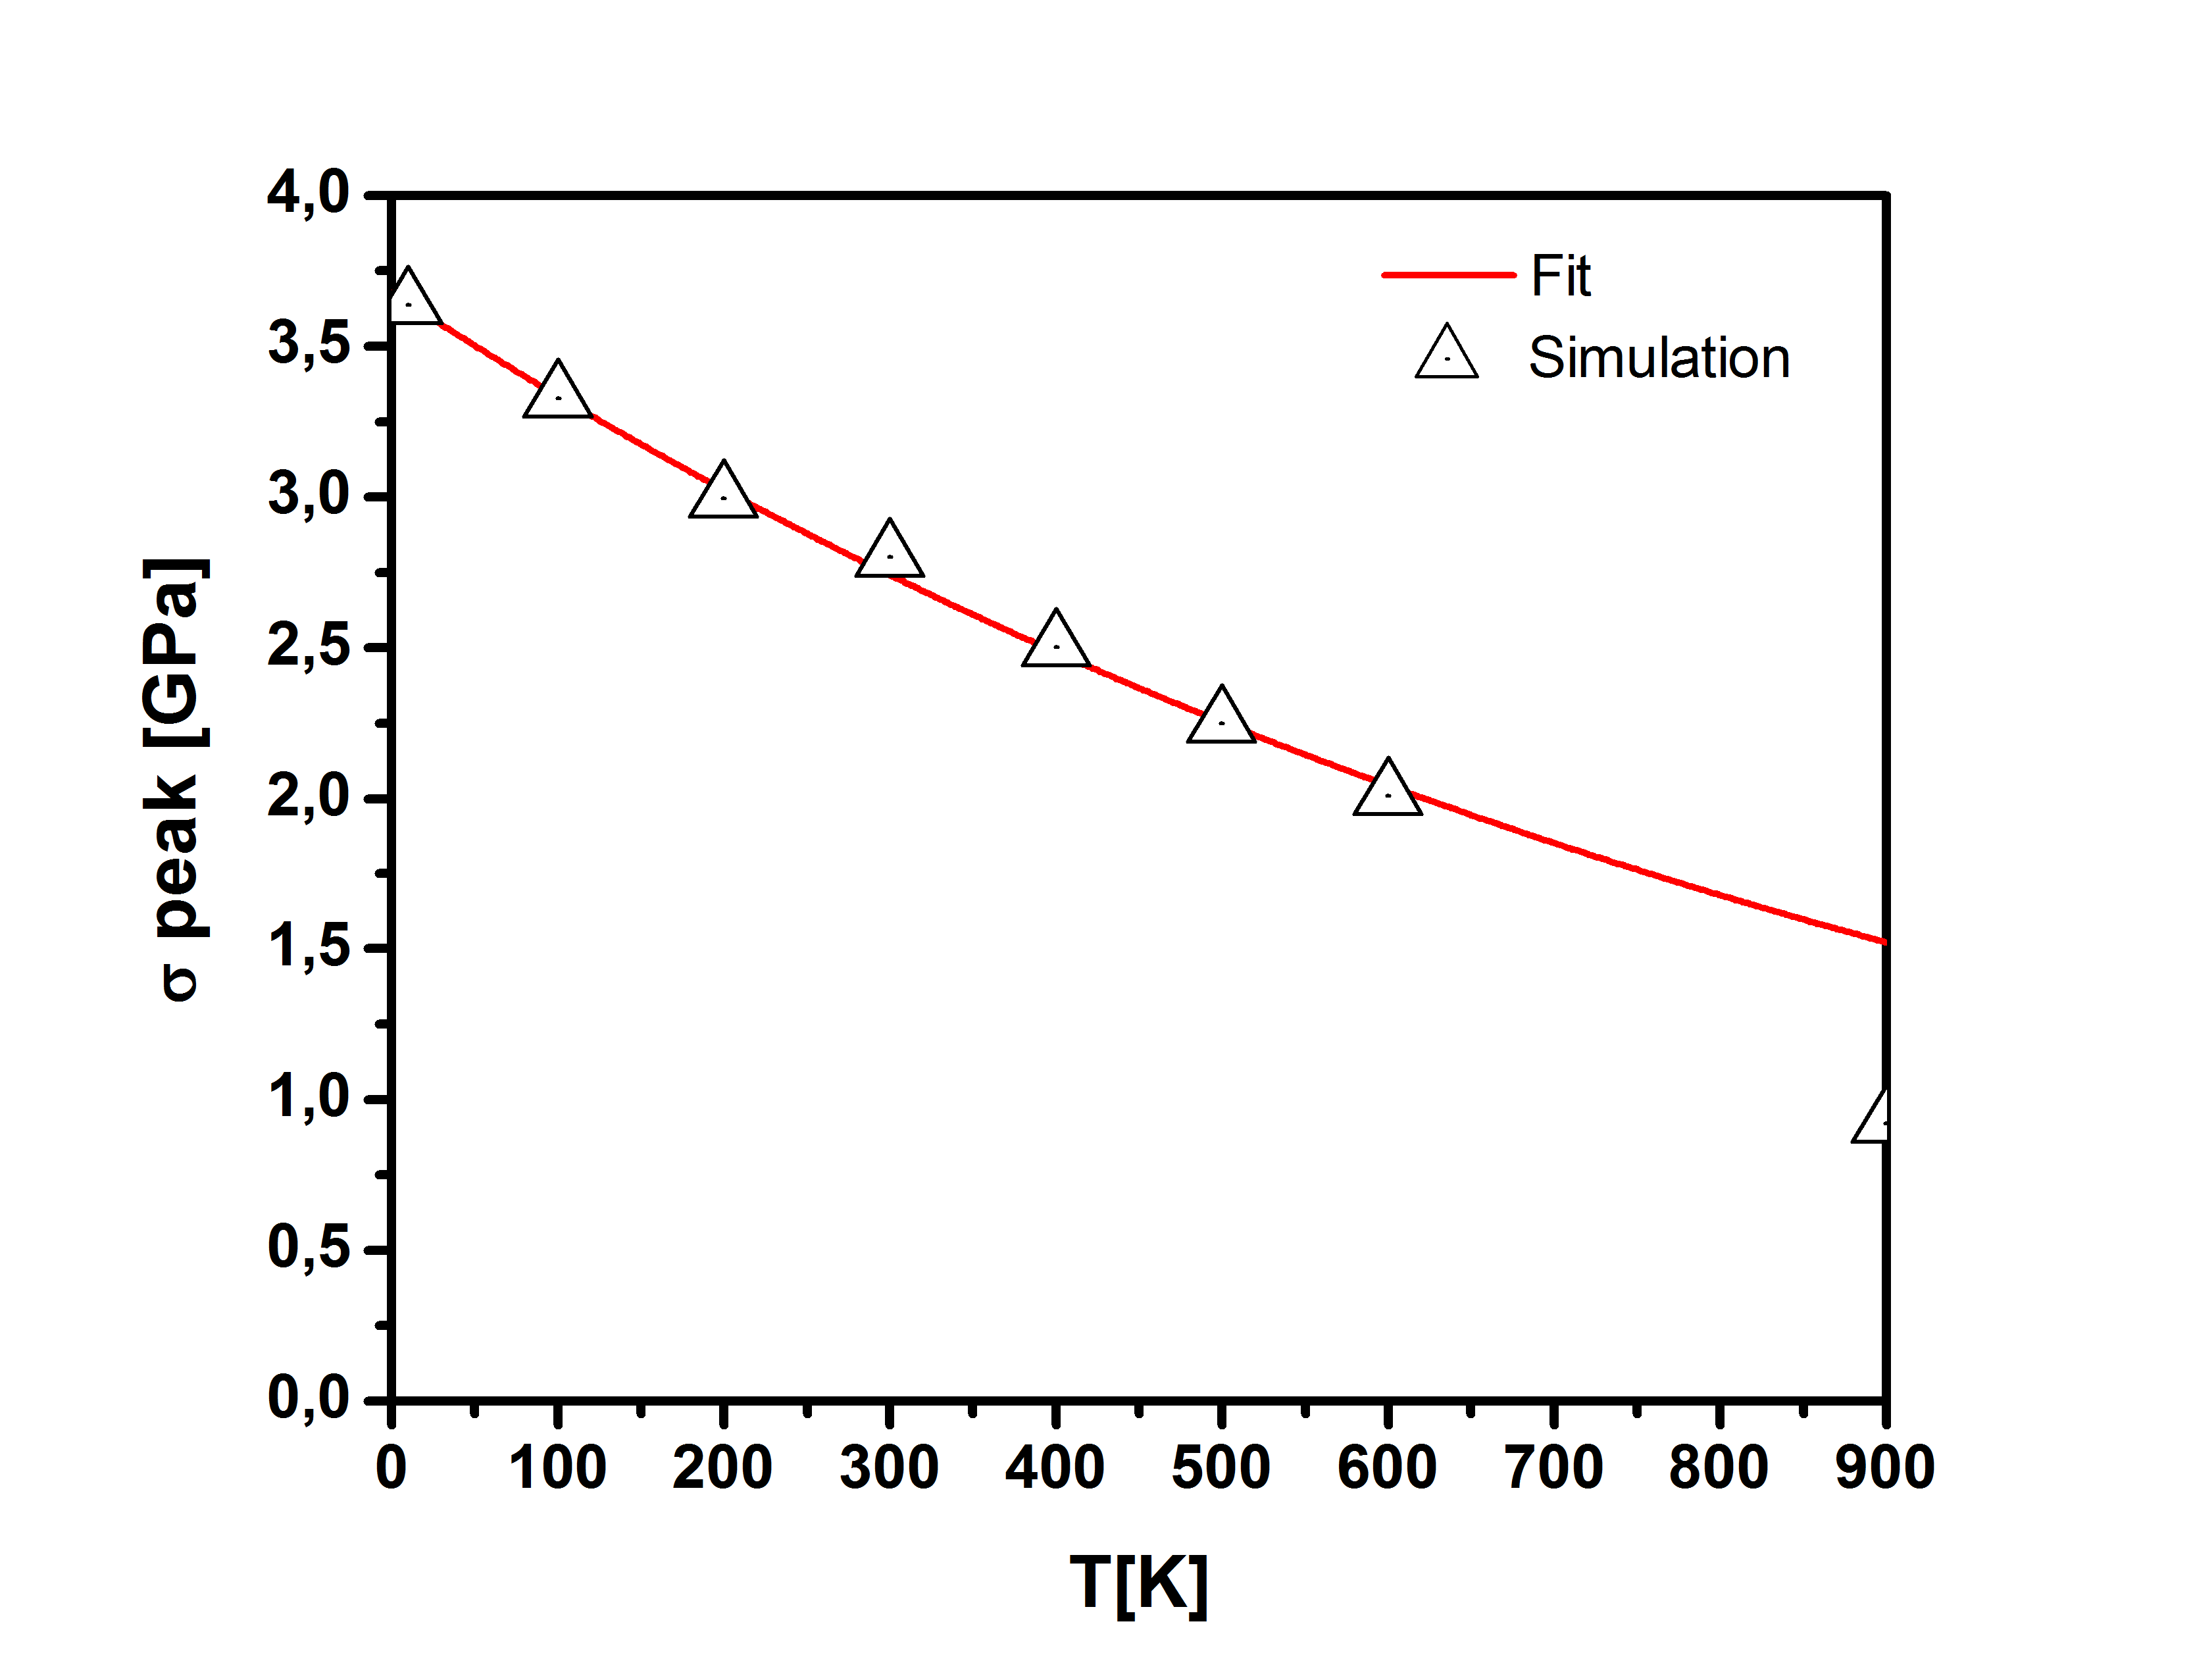
\includegraphics[width=8cm]{Figures/peakstress_T_COMP.png}
\caption{Von Mises maximo vs. Temperatura}
\end{figure}

\begin{figure}[H]
\centering
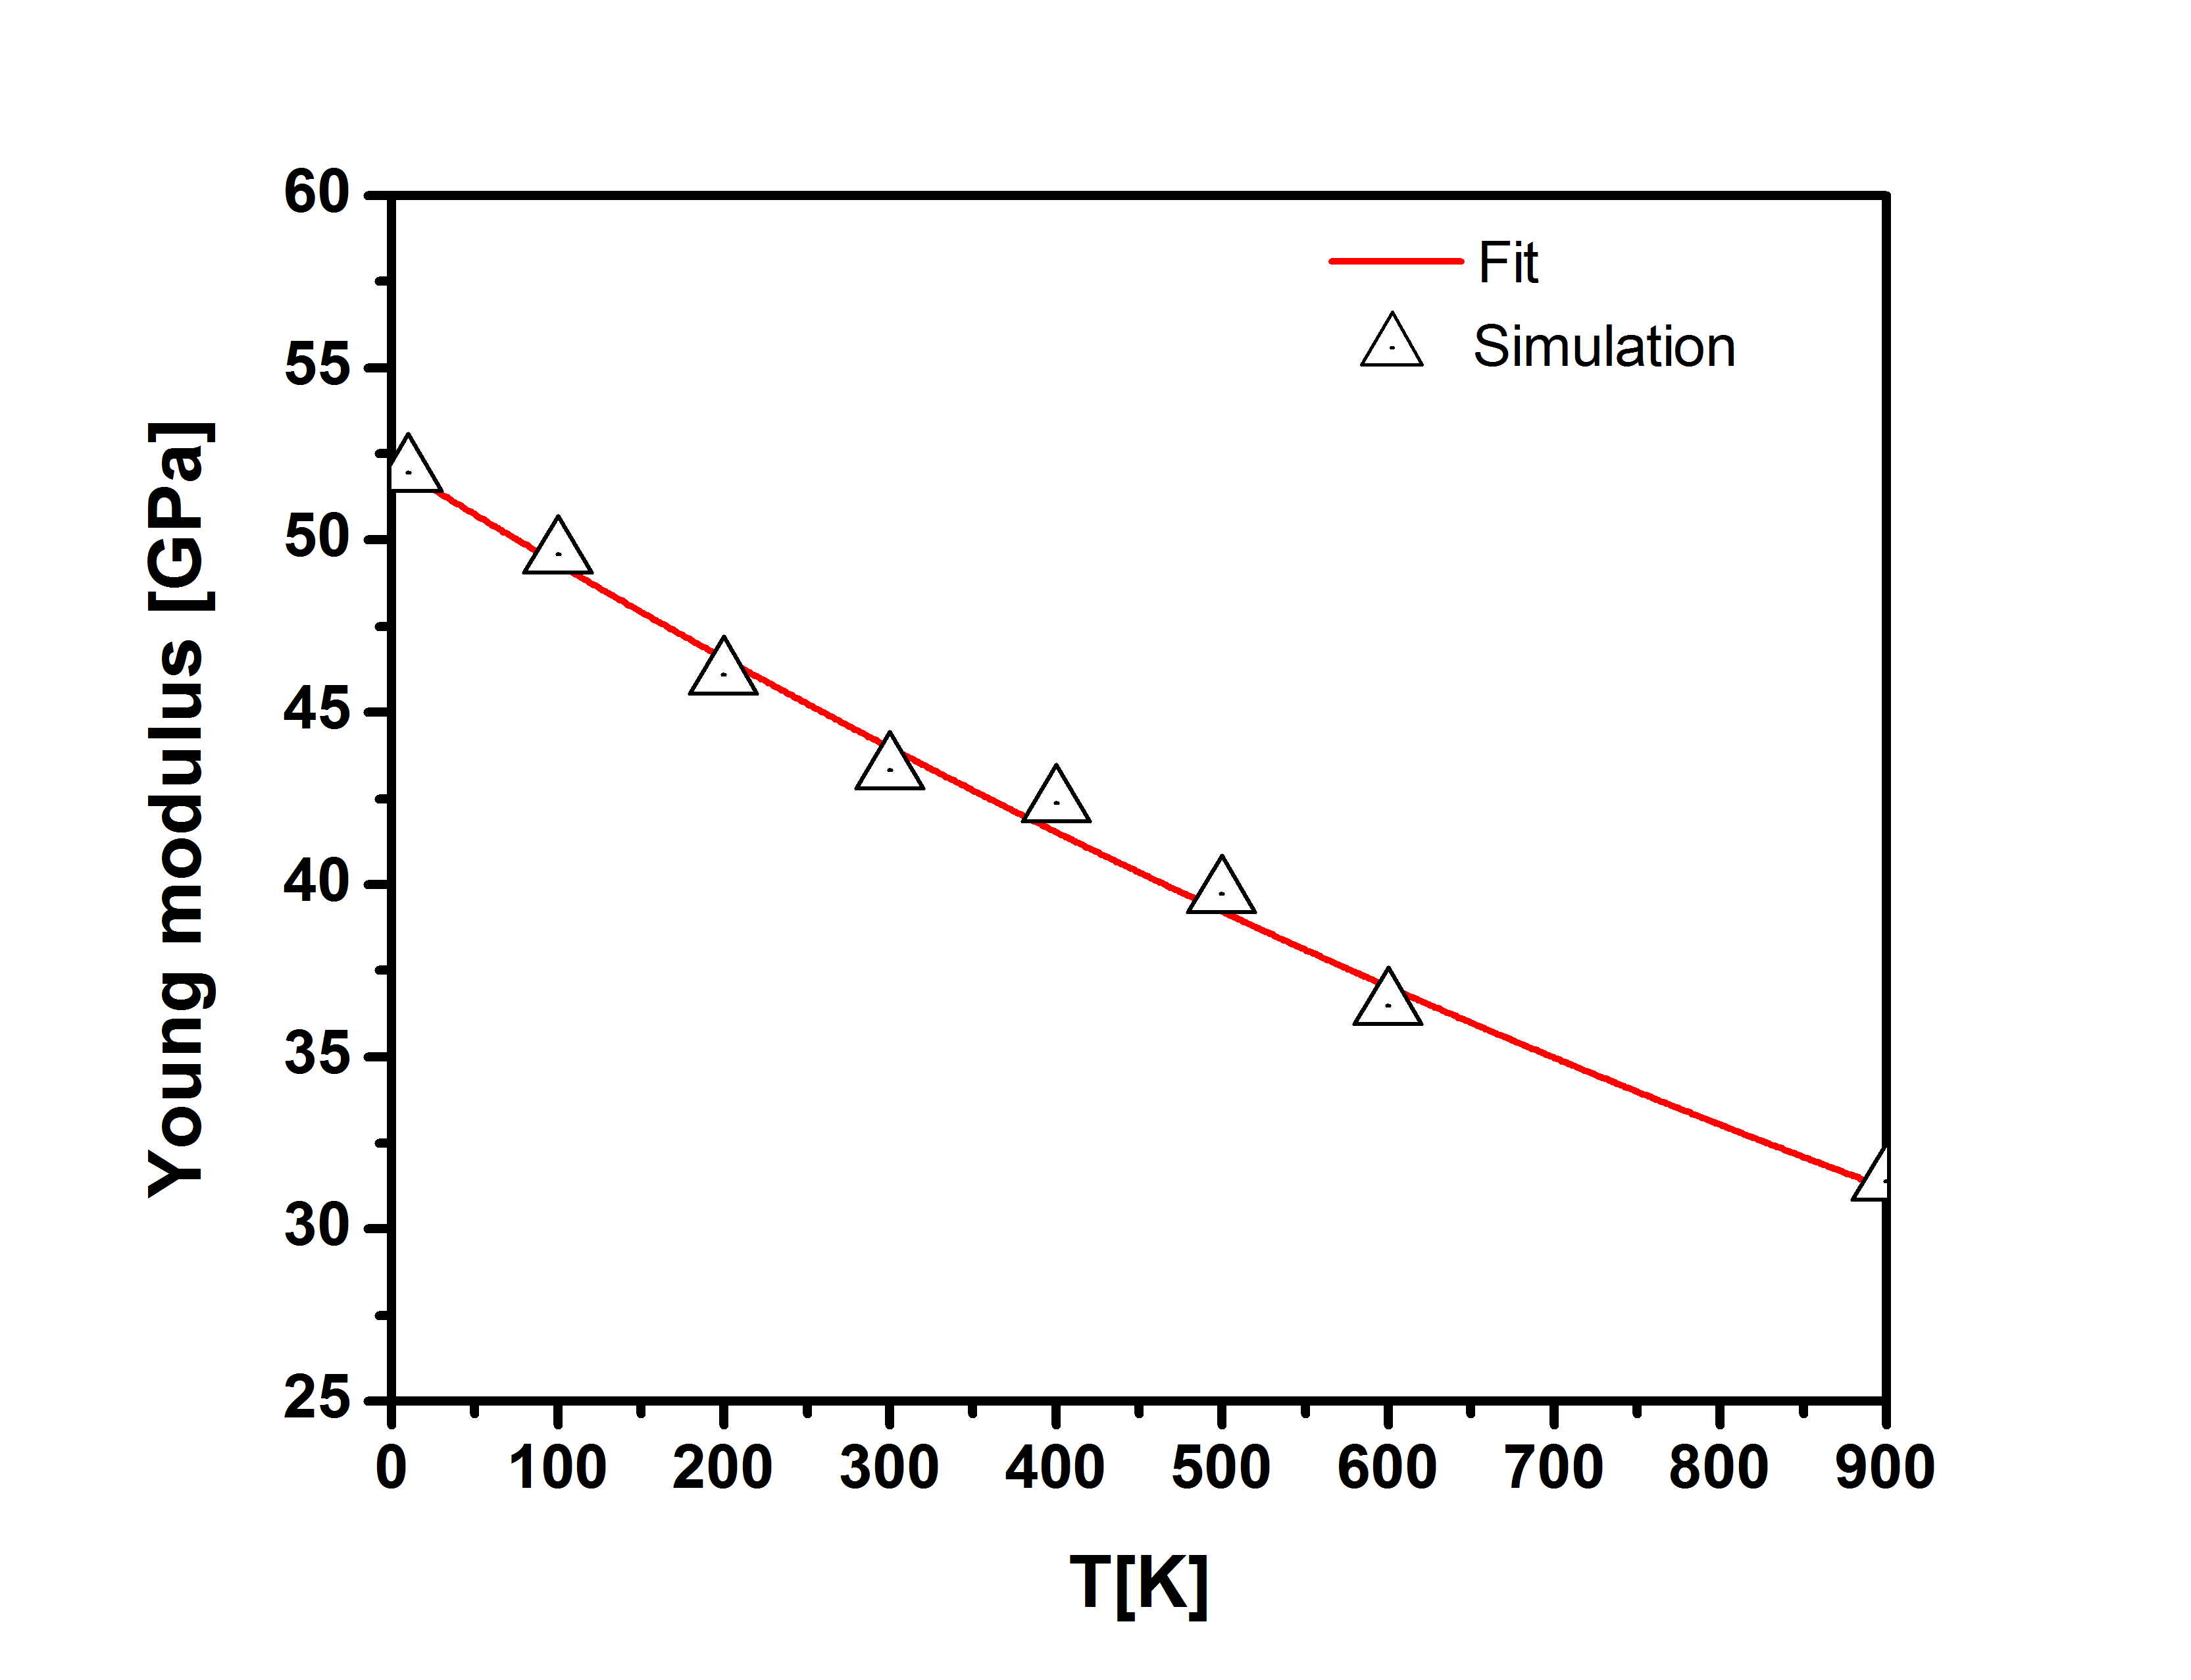
\includegraphics[width=8cm]{Figures/young_T_COMP.png}
\caption{Modulo Young vs. Temperatura}
\end{figure}

\begin{figure}[H]
\centering
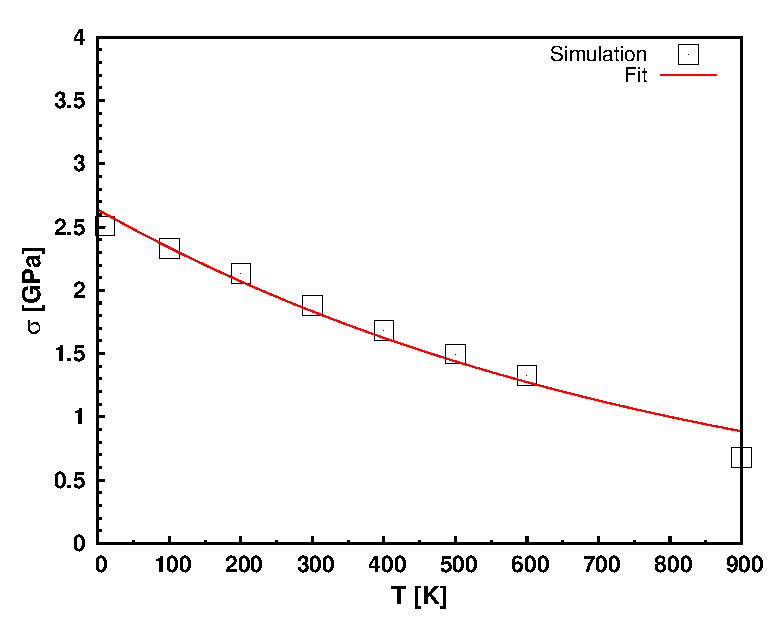
\includegraphics[width=8cm]{Figures/18stress_T_COMP.eps}
\caption{Von Mises a strain 18\% vs. Temperatura}
\end{figure}

\begin{figure}[H]
\centering
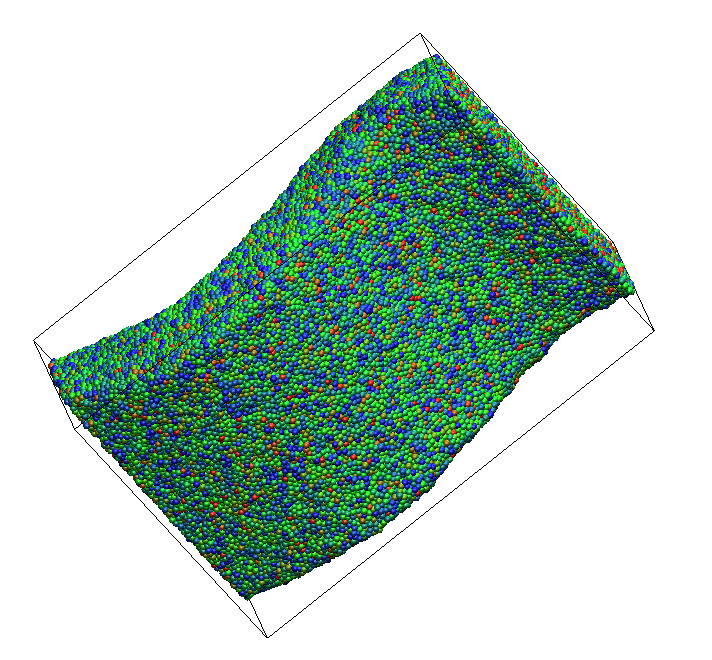
\includegraphics[width=8cm]{Figures/300libresComp.png}
\caption{Muestra a 300K cond. de frontera libres strain 20\%}
\end{figure}

\begin{figure}[H]
\centering
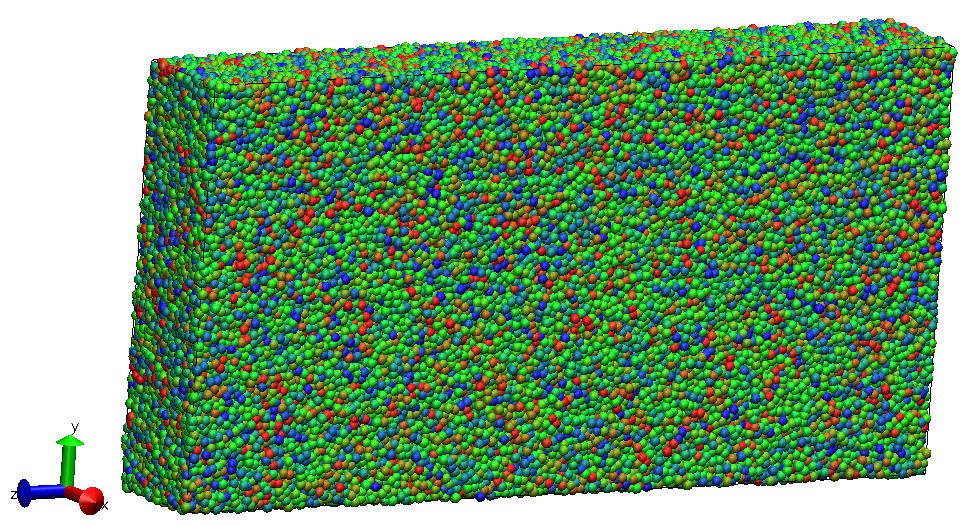
\includegraphics[width=8cm]{Figures/All_300K_6pstrain_sacale100-400_Comp.png}
\caption{Muestra a 300K cond. de frontera periodicas, 6\% strain, escala de colores 100-400 GPa}
\end{figure}

\begin{figure}[H]
\centering
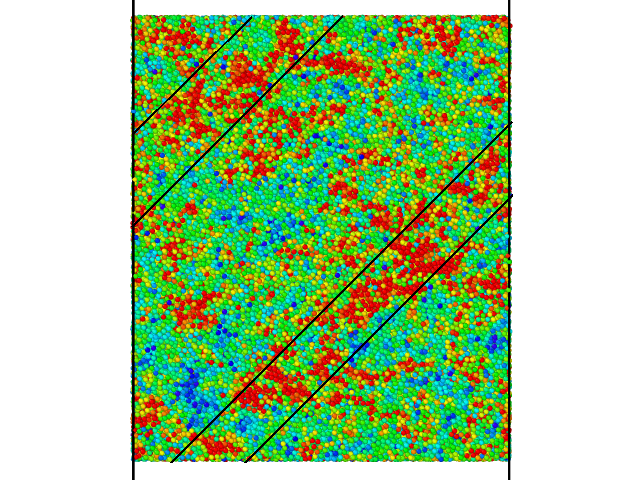
\includegraphics[width=8cm]{Figures/ShearBand.png}
\caption{Shearband a 300K, 14\% strain, escala 0.02 a 0.15 atomic strain}
\end{figure}

\begin{figure}[H]
\centering
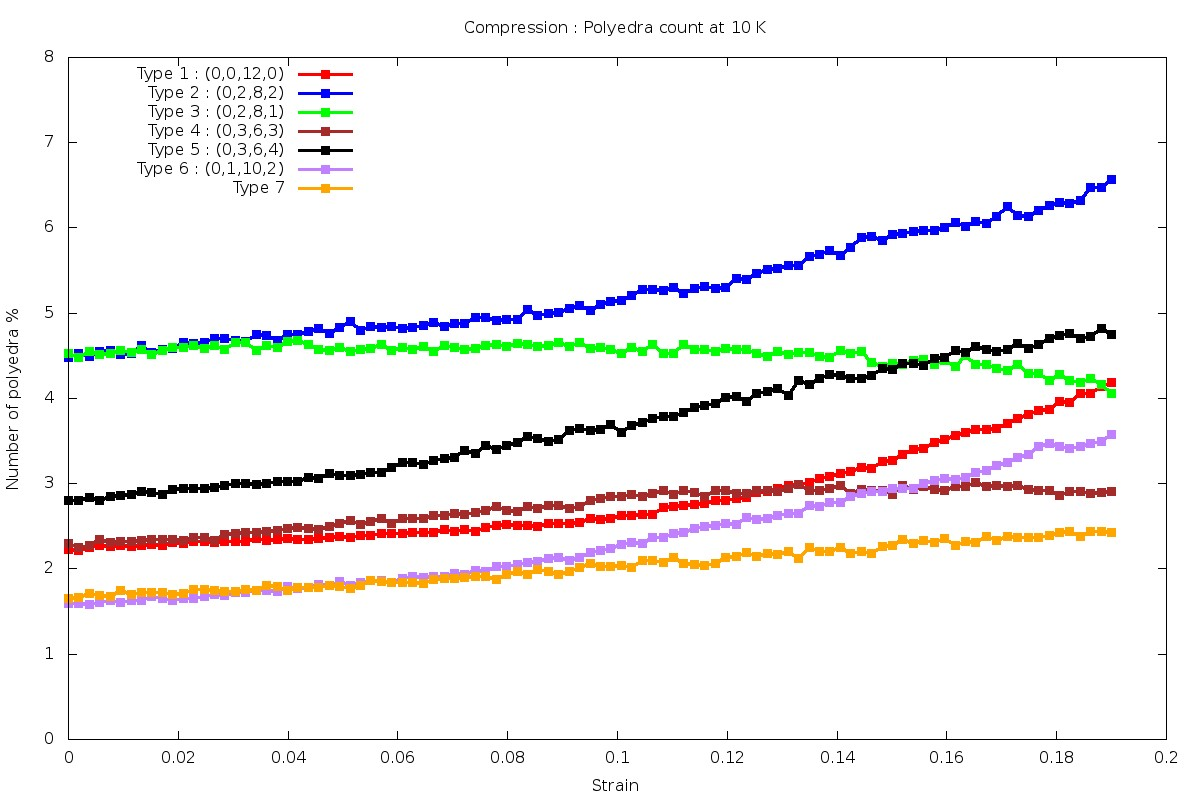
\includegraphics[width=8cm]{Figures/Compr_Polyedra_10K.jpeg}
\caption{Polyedros de voronoi vs. strain para 10K}
\end{figure}

\begin{figure}[H]
\centering
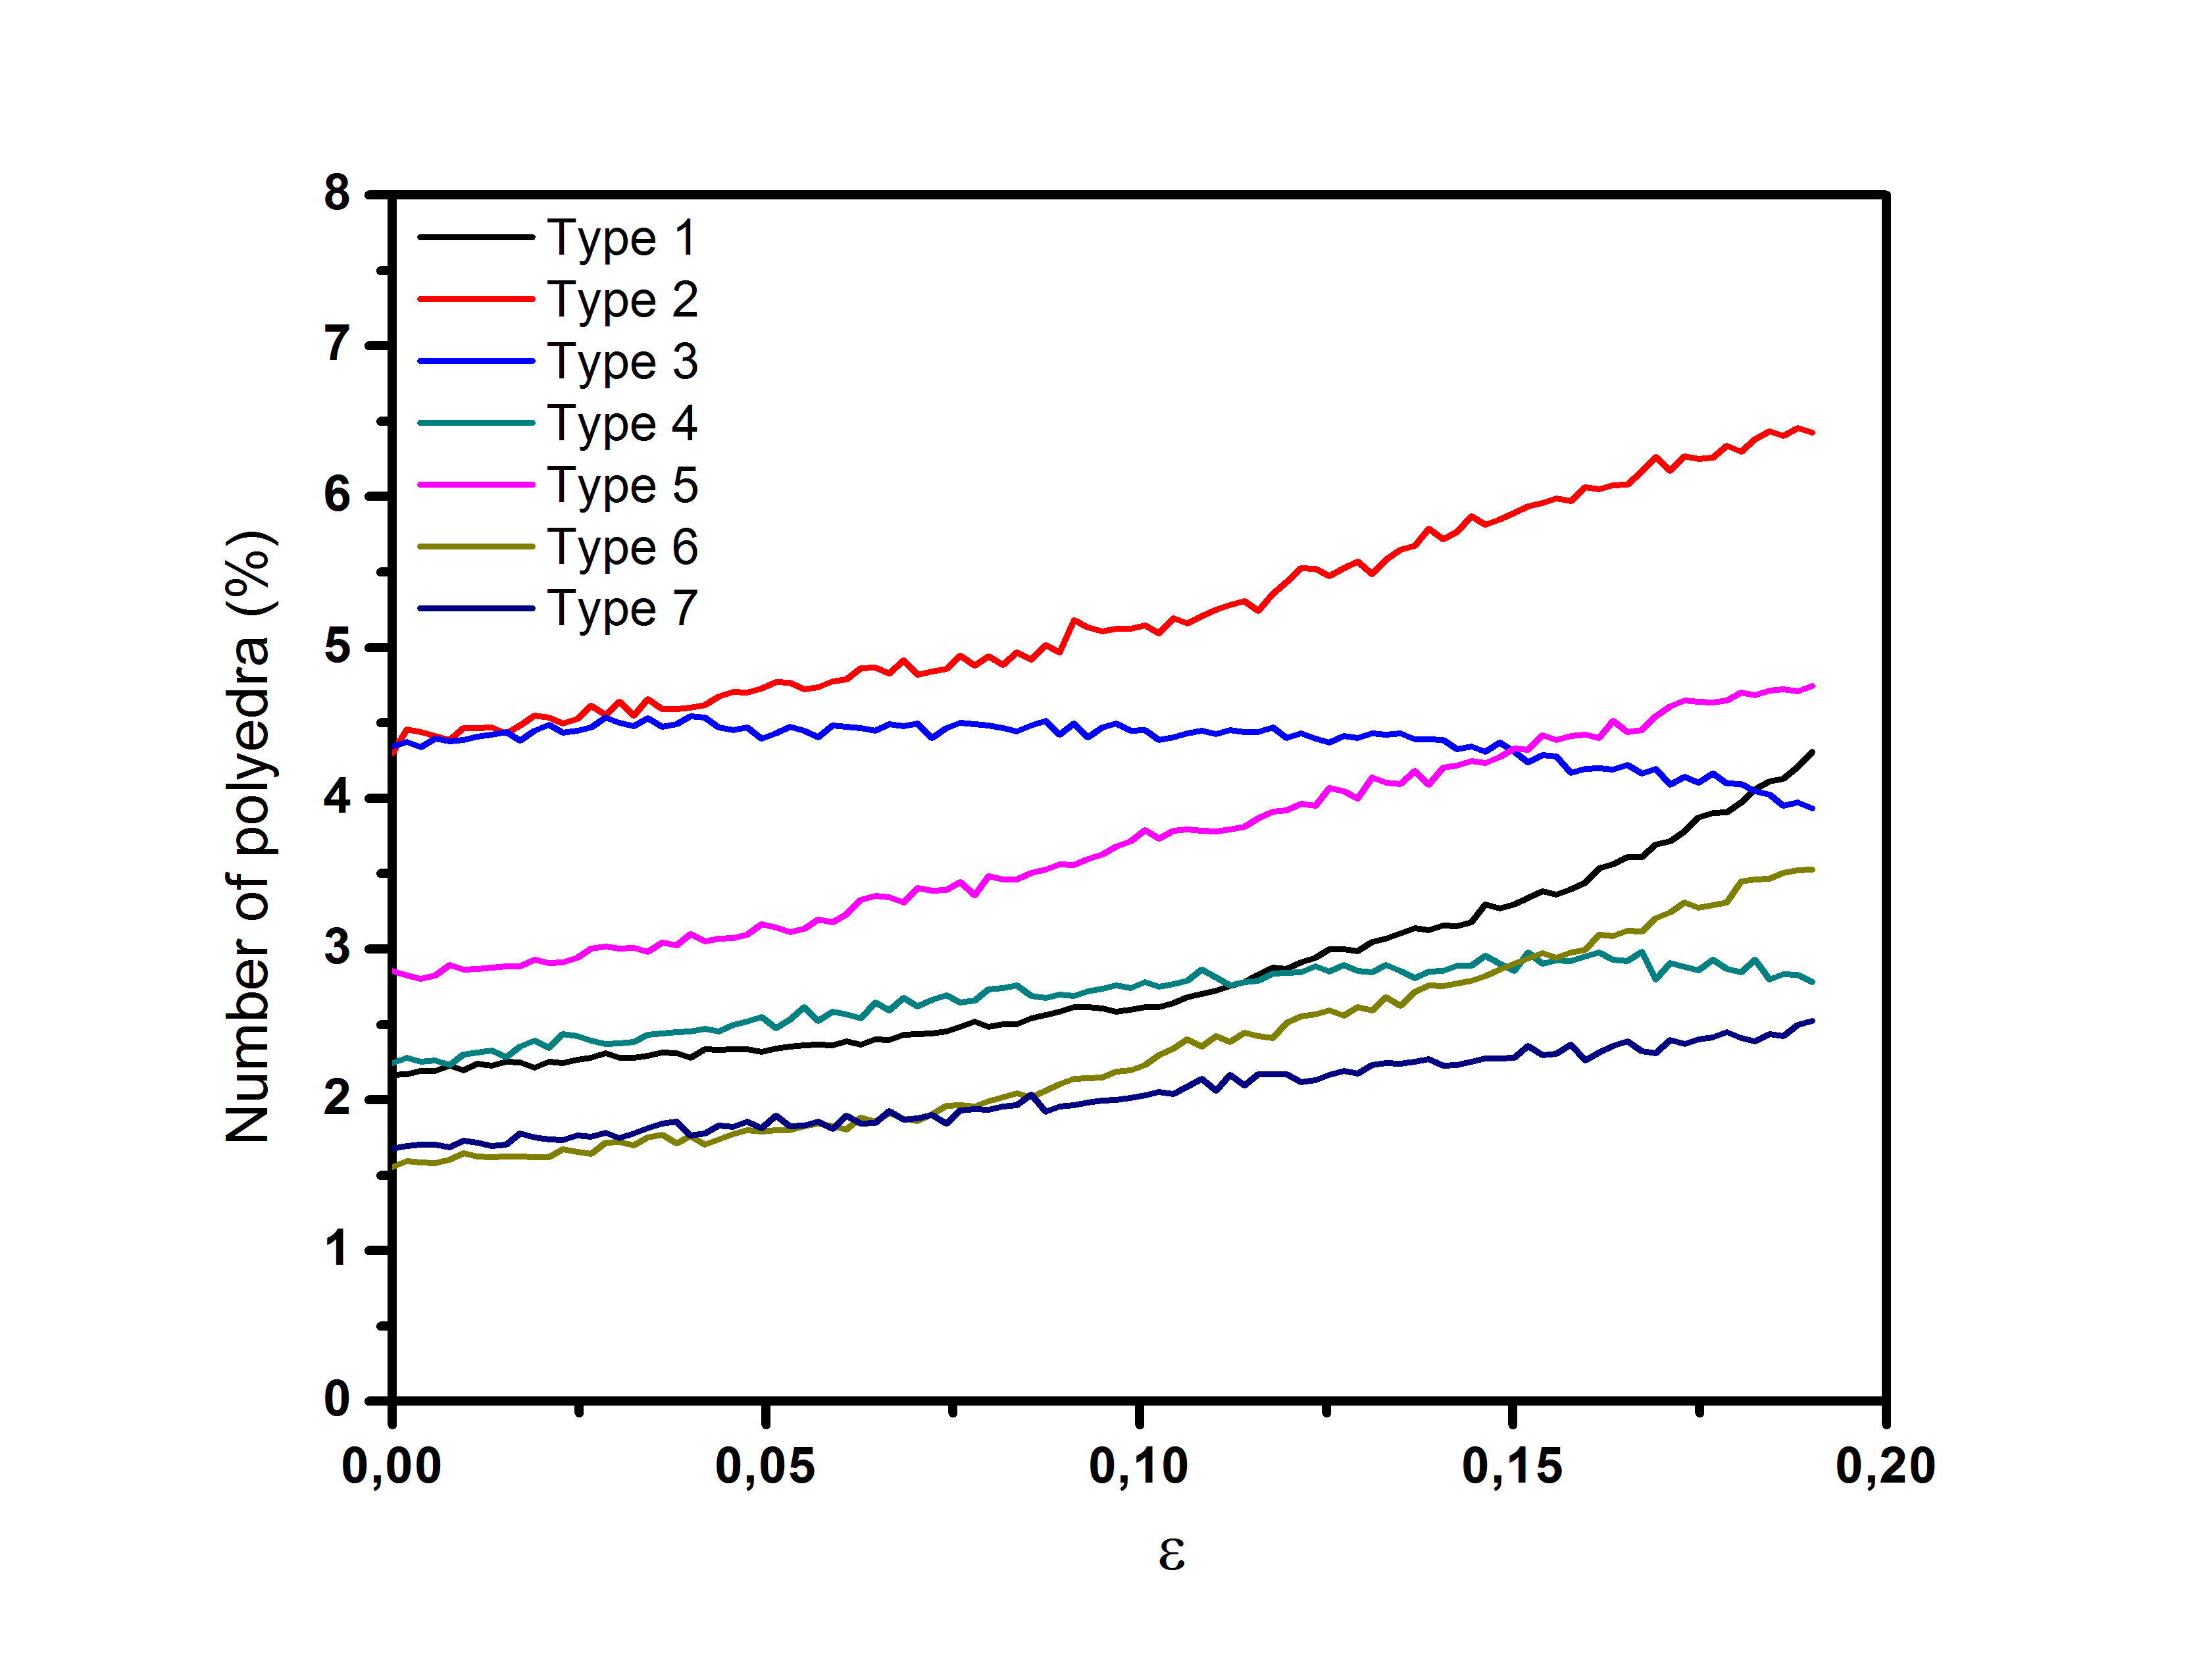
\includegraphics[width=8cm]{Figures/Polyedra_Vs_Strain_100K_COMP.png}
\caption{Num polyedros de voronoi vs. strain, a 100K}
\end{figure}

\begin{figure}[H]
\centering
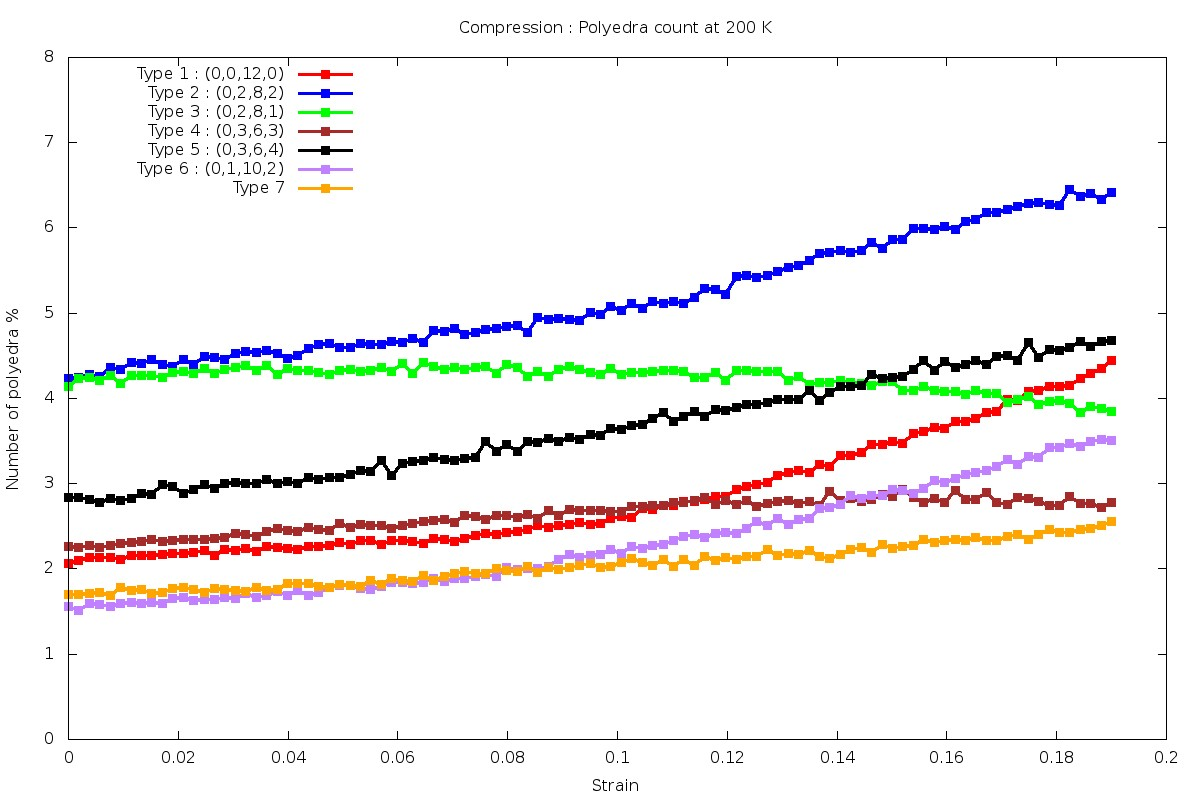
\includegraphics[width=8cm]{Figures/Compr_Polyedra_200K.jpeg}
\caption{Polyedros de voronoi vs. strain para 200K}
\end{figure}

\begin{figure}[H]
\centering
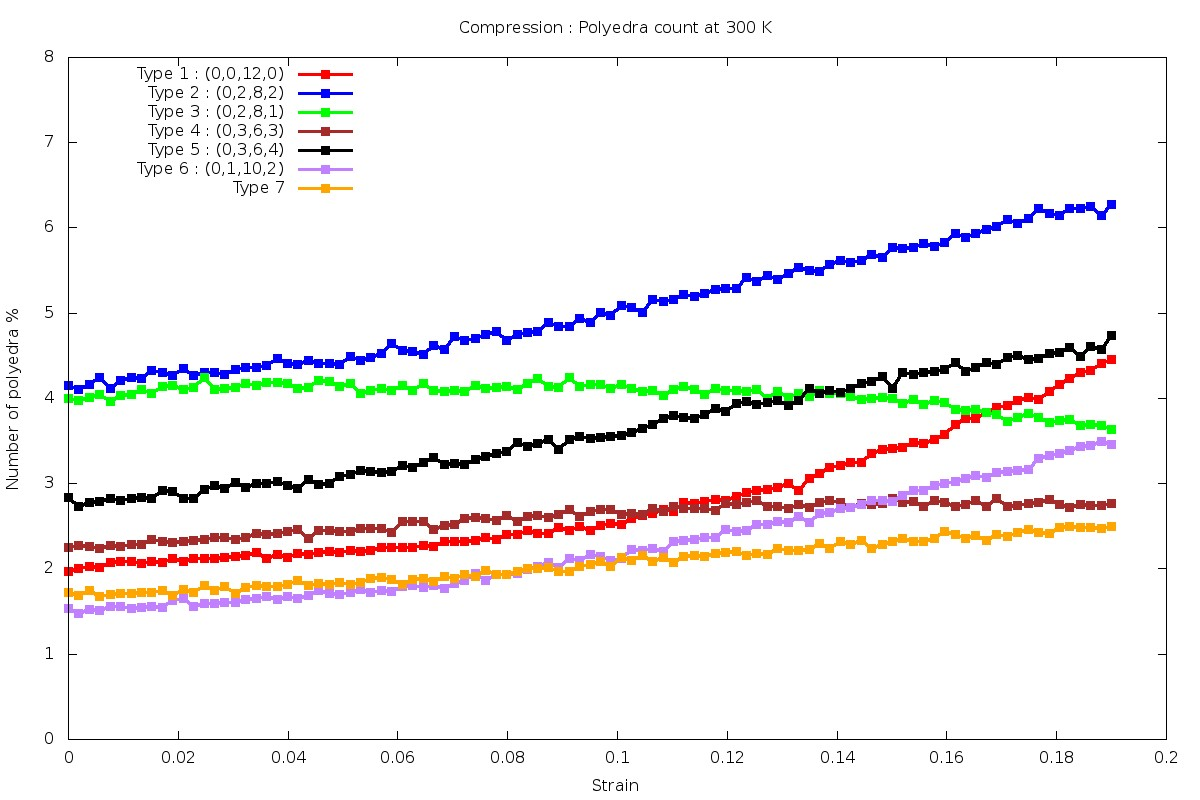
\includegraphics[width=8cm]{Figures/Compr_Polyedra_300K.jpeg}
\caption{Polyedros de voronoi vs. strain para 300K}
\end{figure}

\begin{figure}[H]
\centering
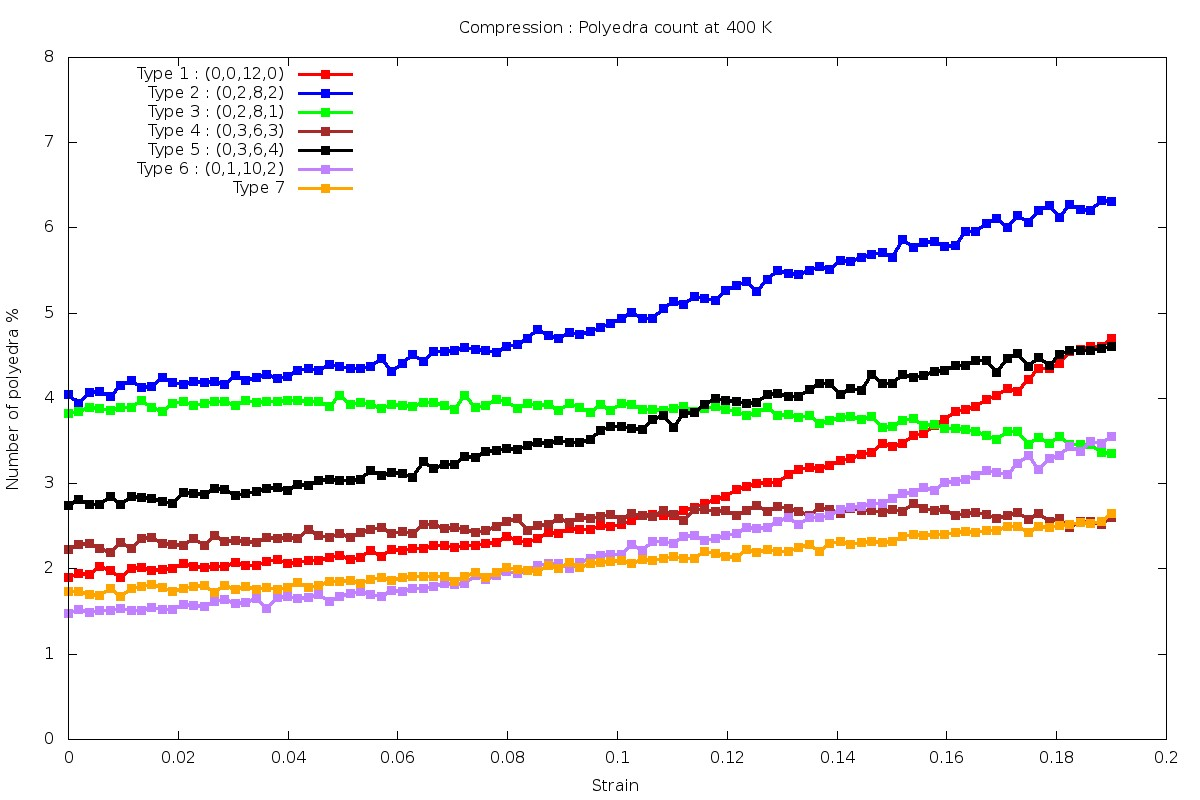
\includegraphics[width=8cm]{Figures/Compr_Polyedra_400K.jpeg}
\caption{Polyedros de voronoi vs. strain para 400K}
\end{figure}

\begin{figure}[H]
\centering
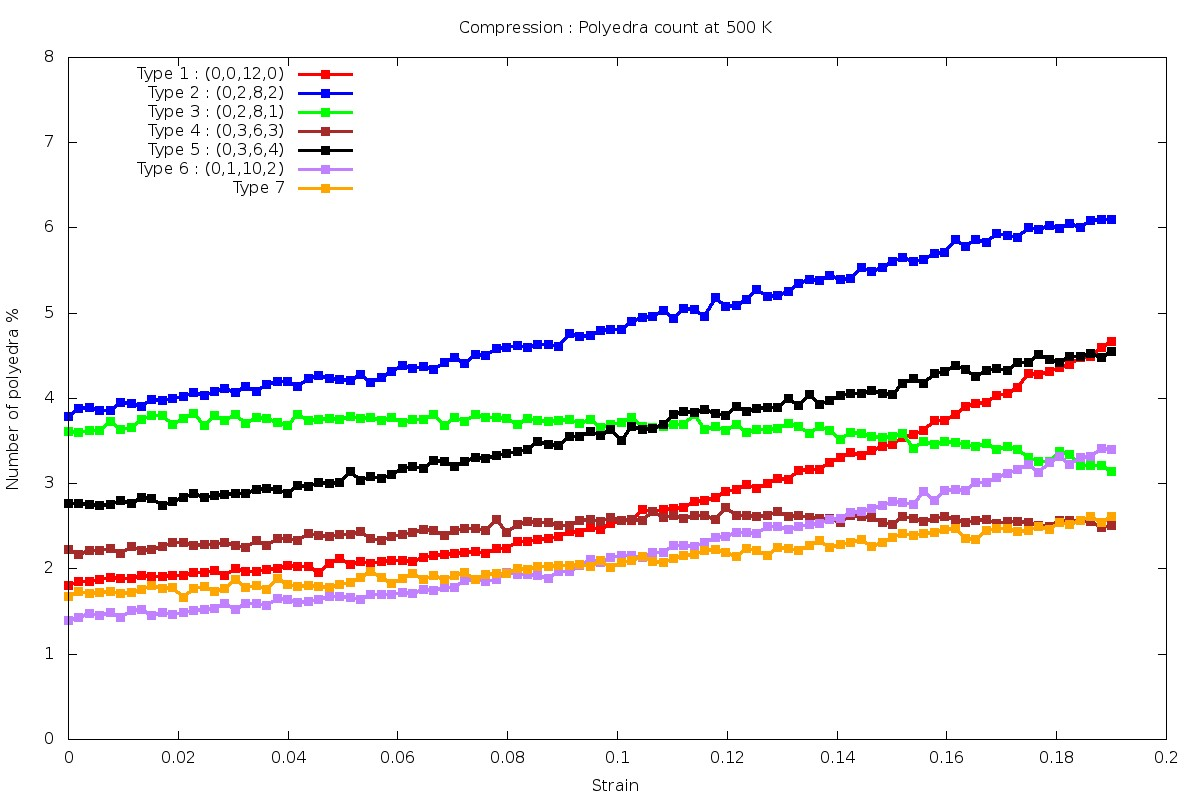
\includegraphics[width=8cm]{Figures/Compr_Polyedra_500K.jpeg}
\caption{Polyedros de voronoi vs. strain para 500K}
\end{figure}

\begin{figure}[H]
\centering
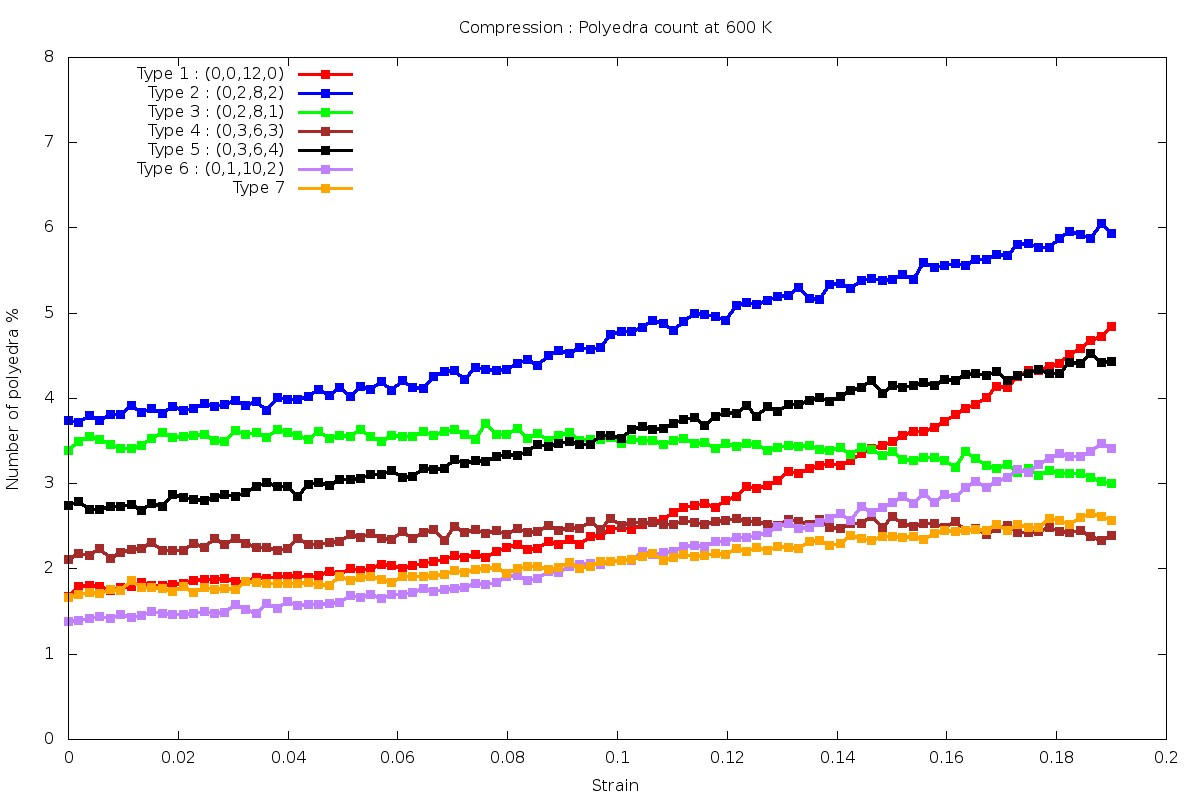
\includegraphics[width=8cm]{Figures/Compr_Polyedra_600K.jpeg}
\caption{Polyedros de voronoi vs. strain para 600K}
\end{figure}

\begin{figure}[H]
\centering
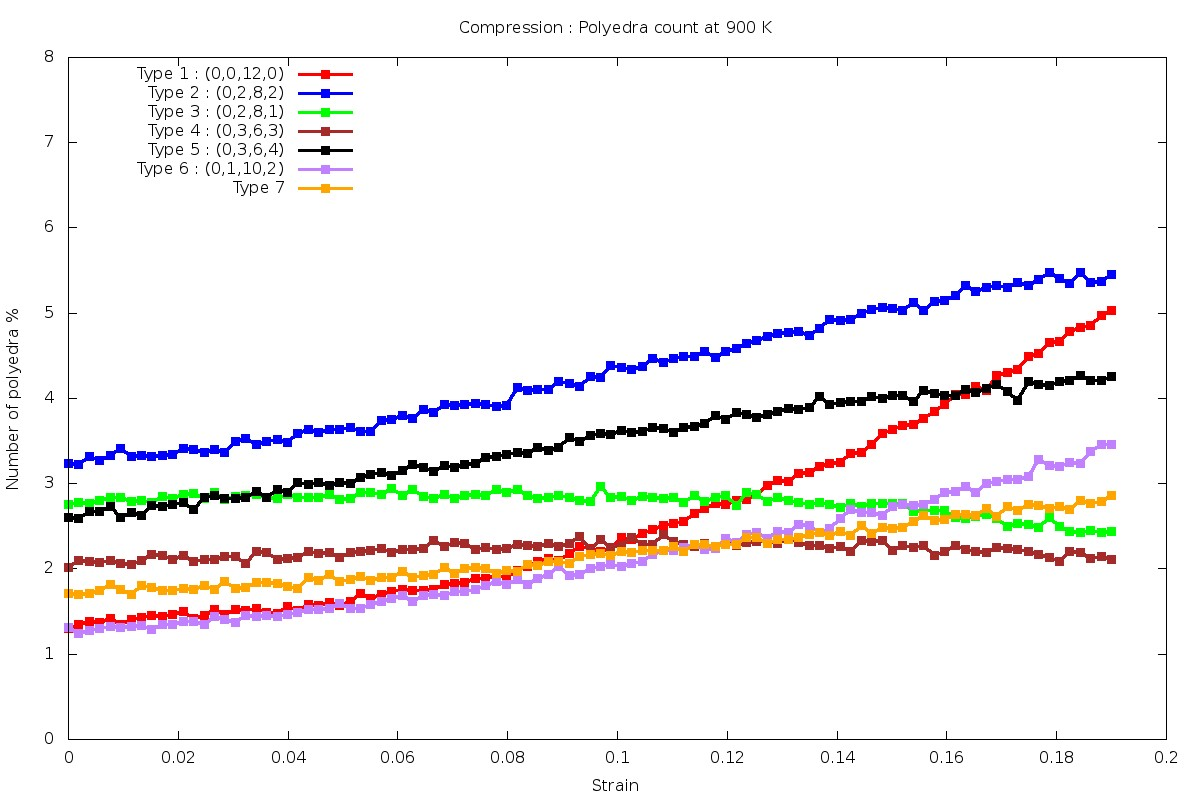
\includegraphics[width=8cm]{Figures/Compr_Polyedra_900K.jpeg}
\caption{Polyedros de voronoi vs. strain para 900K}
\end{figure}

\begin{figure}[H]
\centering
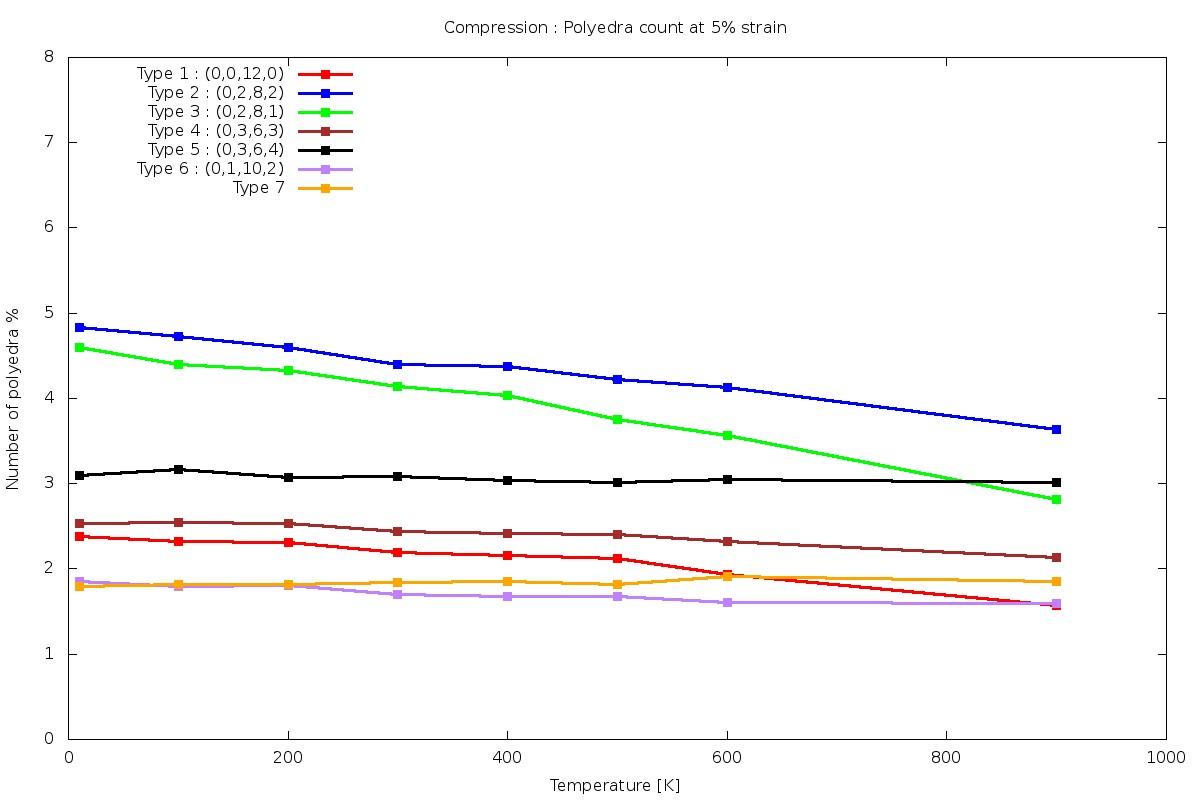
\includegraphics[width=8cm]{Figures/Compr_Voro_Temp_5.jpeg}
\caption{Num polyedros de voronoi vs. temperatura, a strain 5\%}
\end{figure}

\begin{figure}[H]
\centering
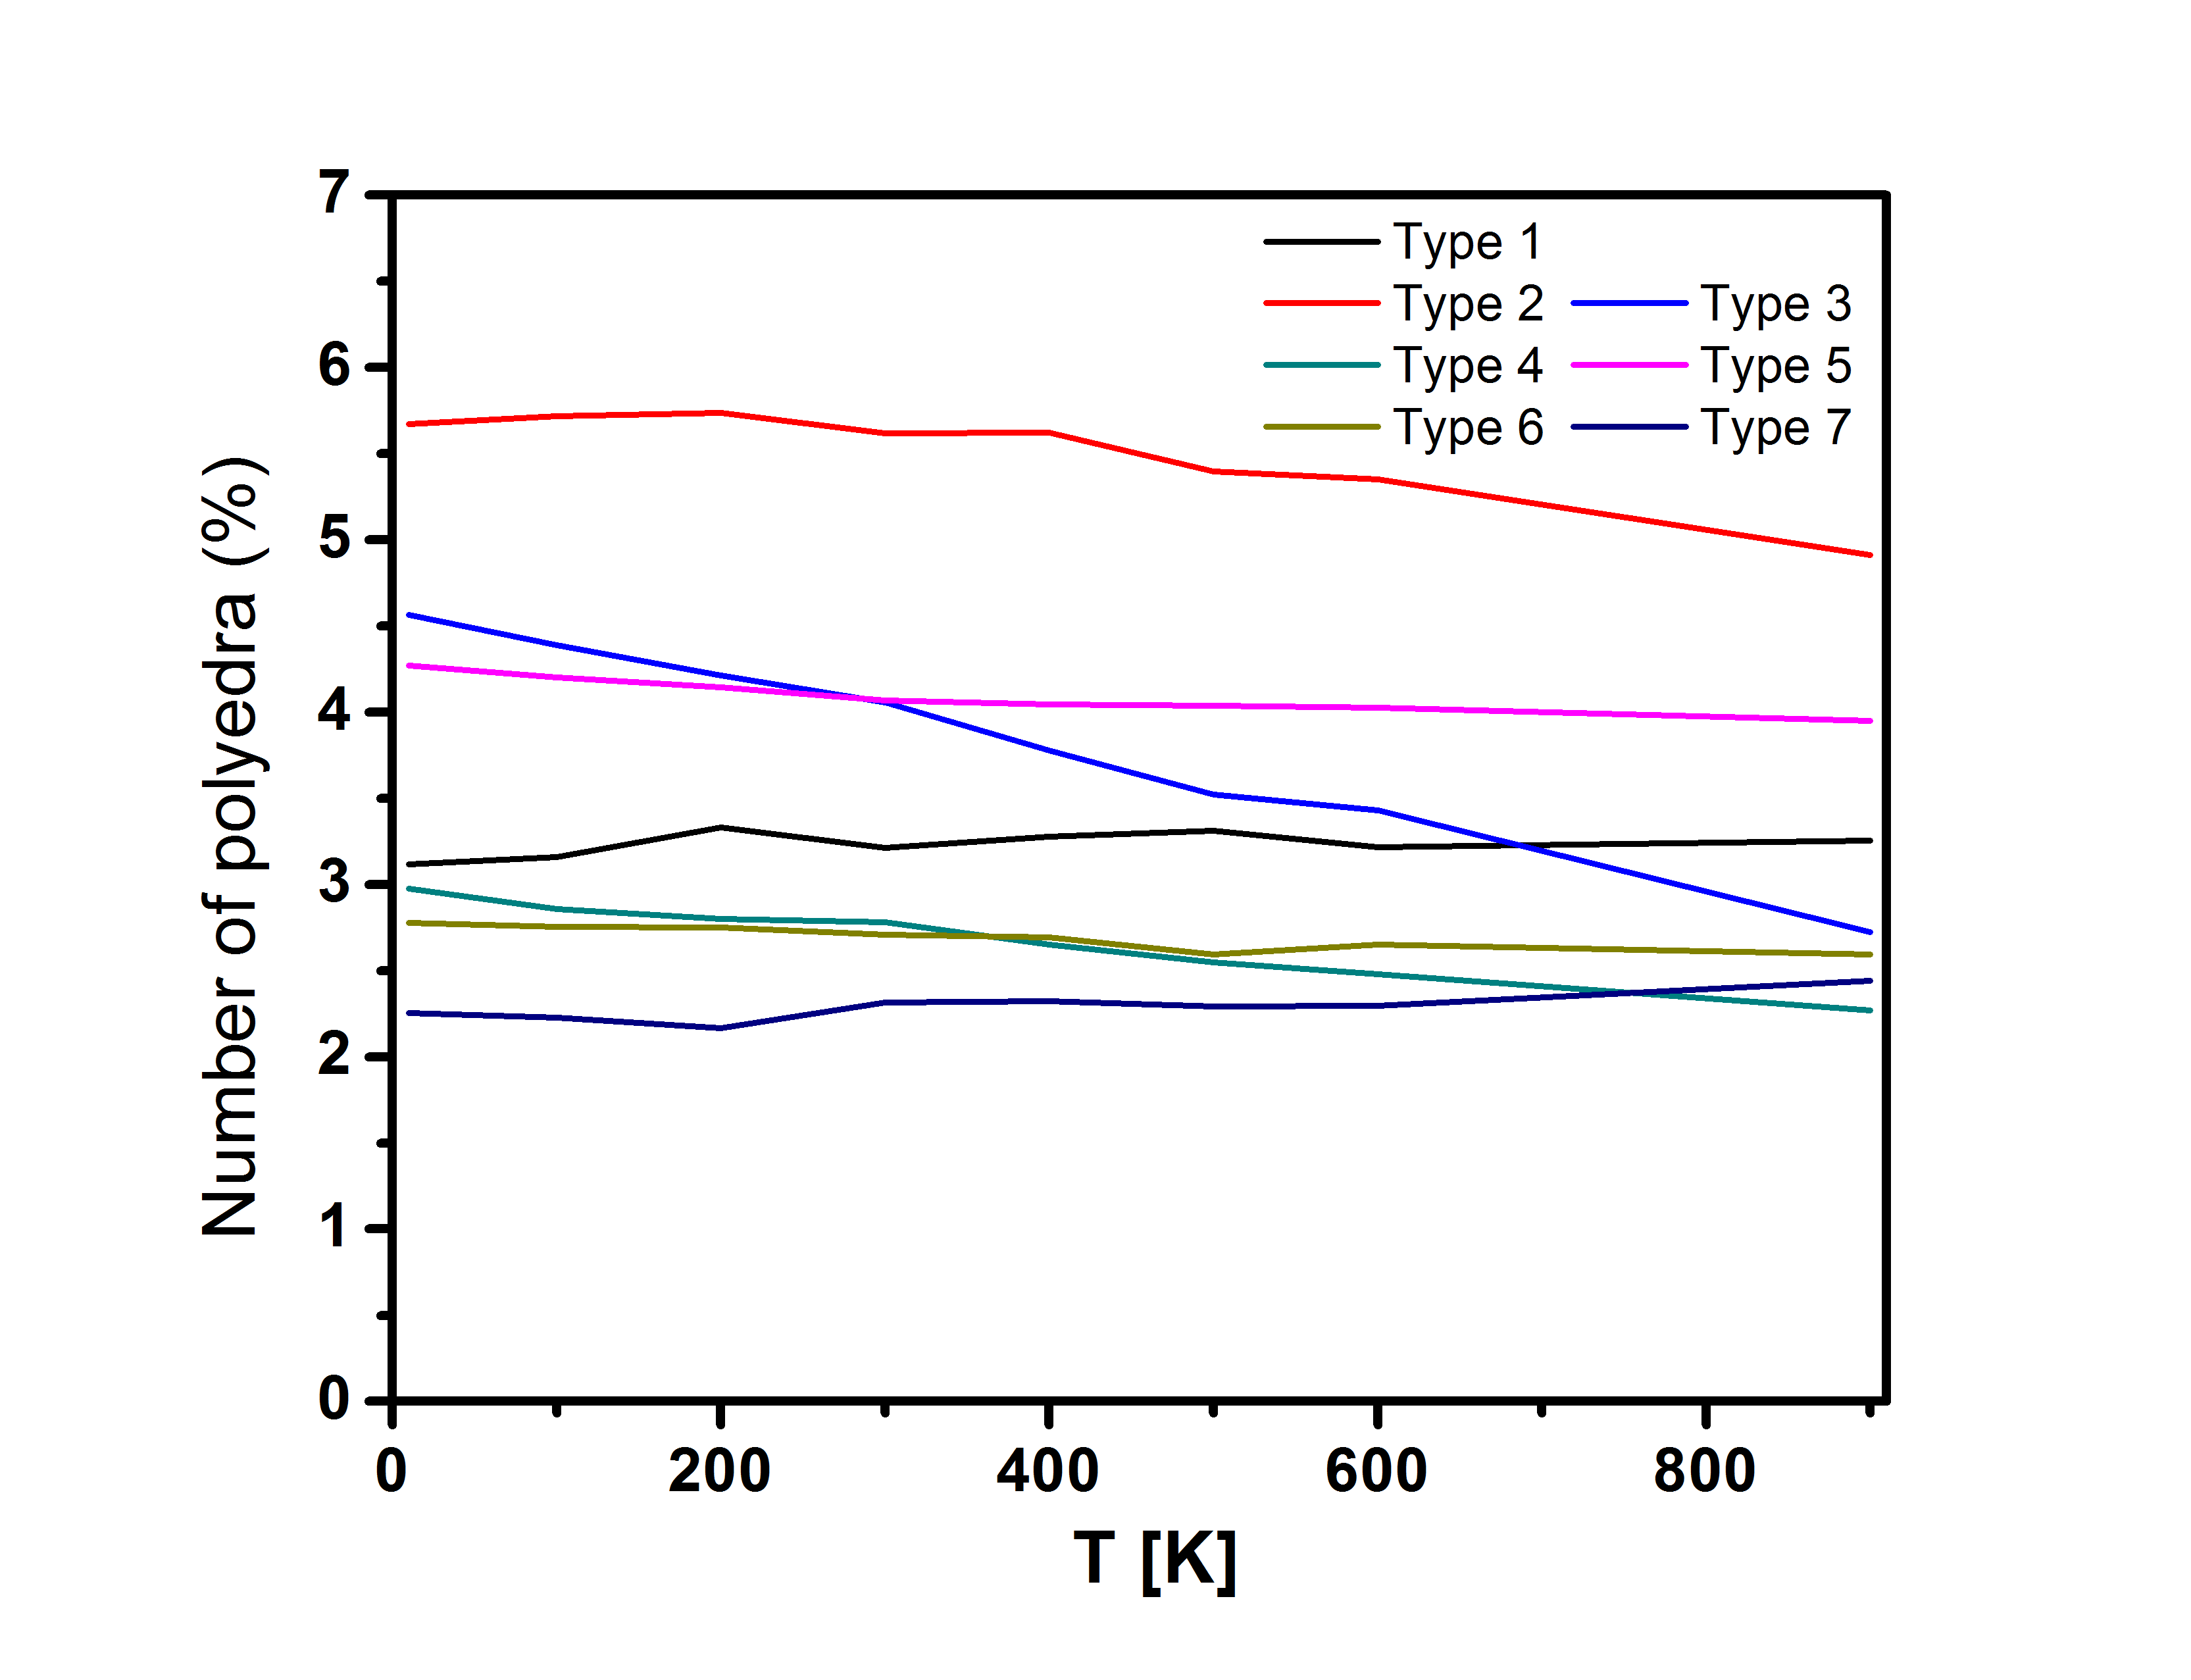
\includegraphics[width=8cm]{Figures/poly_T_14strain_COMP.png}
\caption{Num polyedros de voronoi vs. temperatura, a strain 14\%}
\end{figure}

\begin{figure}[H]
\centering
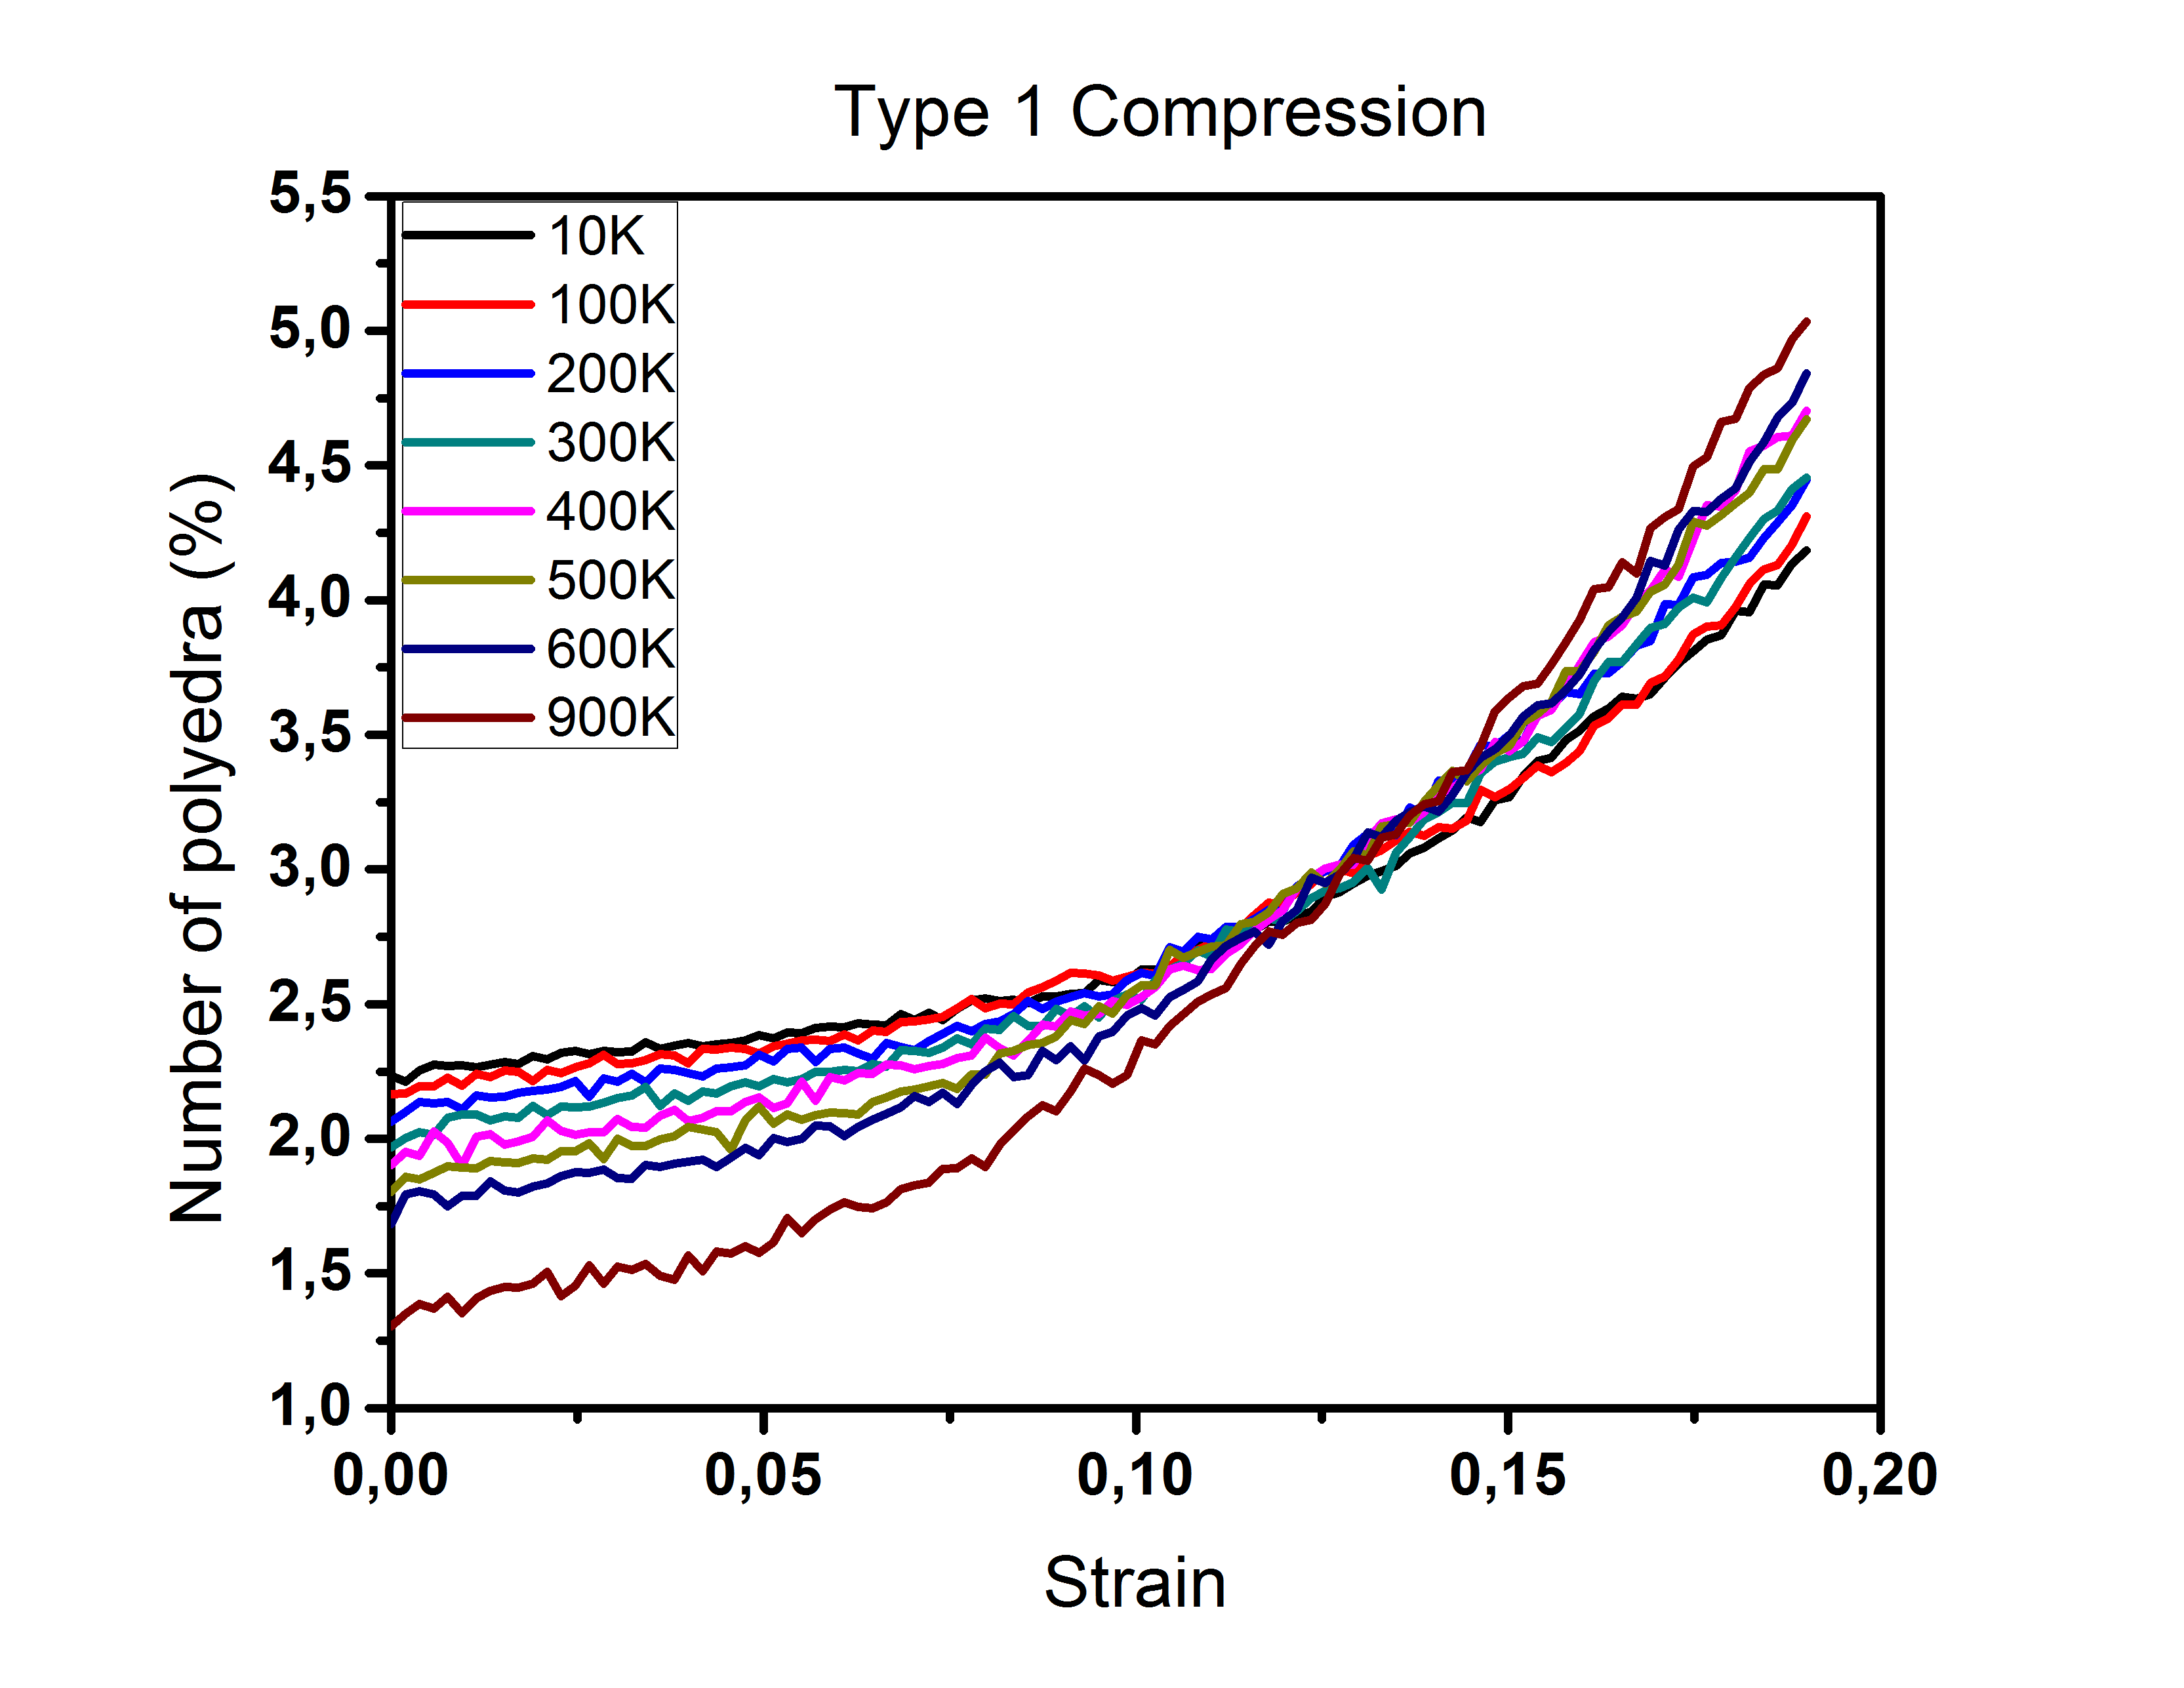
\includegraphics[width=8cm]{Figures/type1_COMP.png}
\caption{polyedros de voronoi tipo 1 vs. strain}
\end{figure}

\begin{figure}[H]
\centering
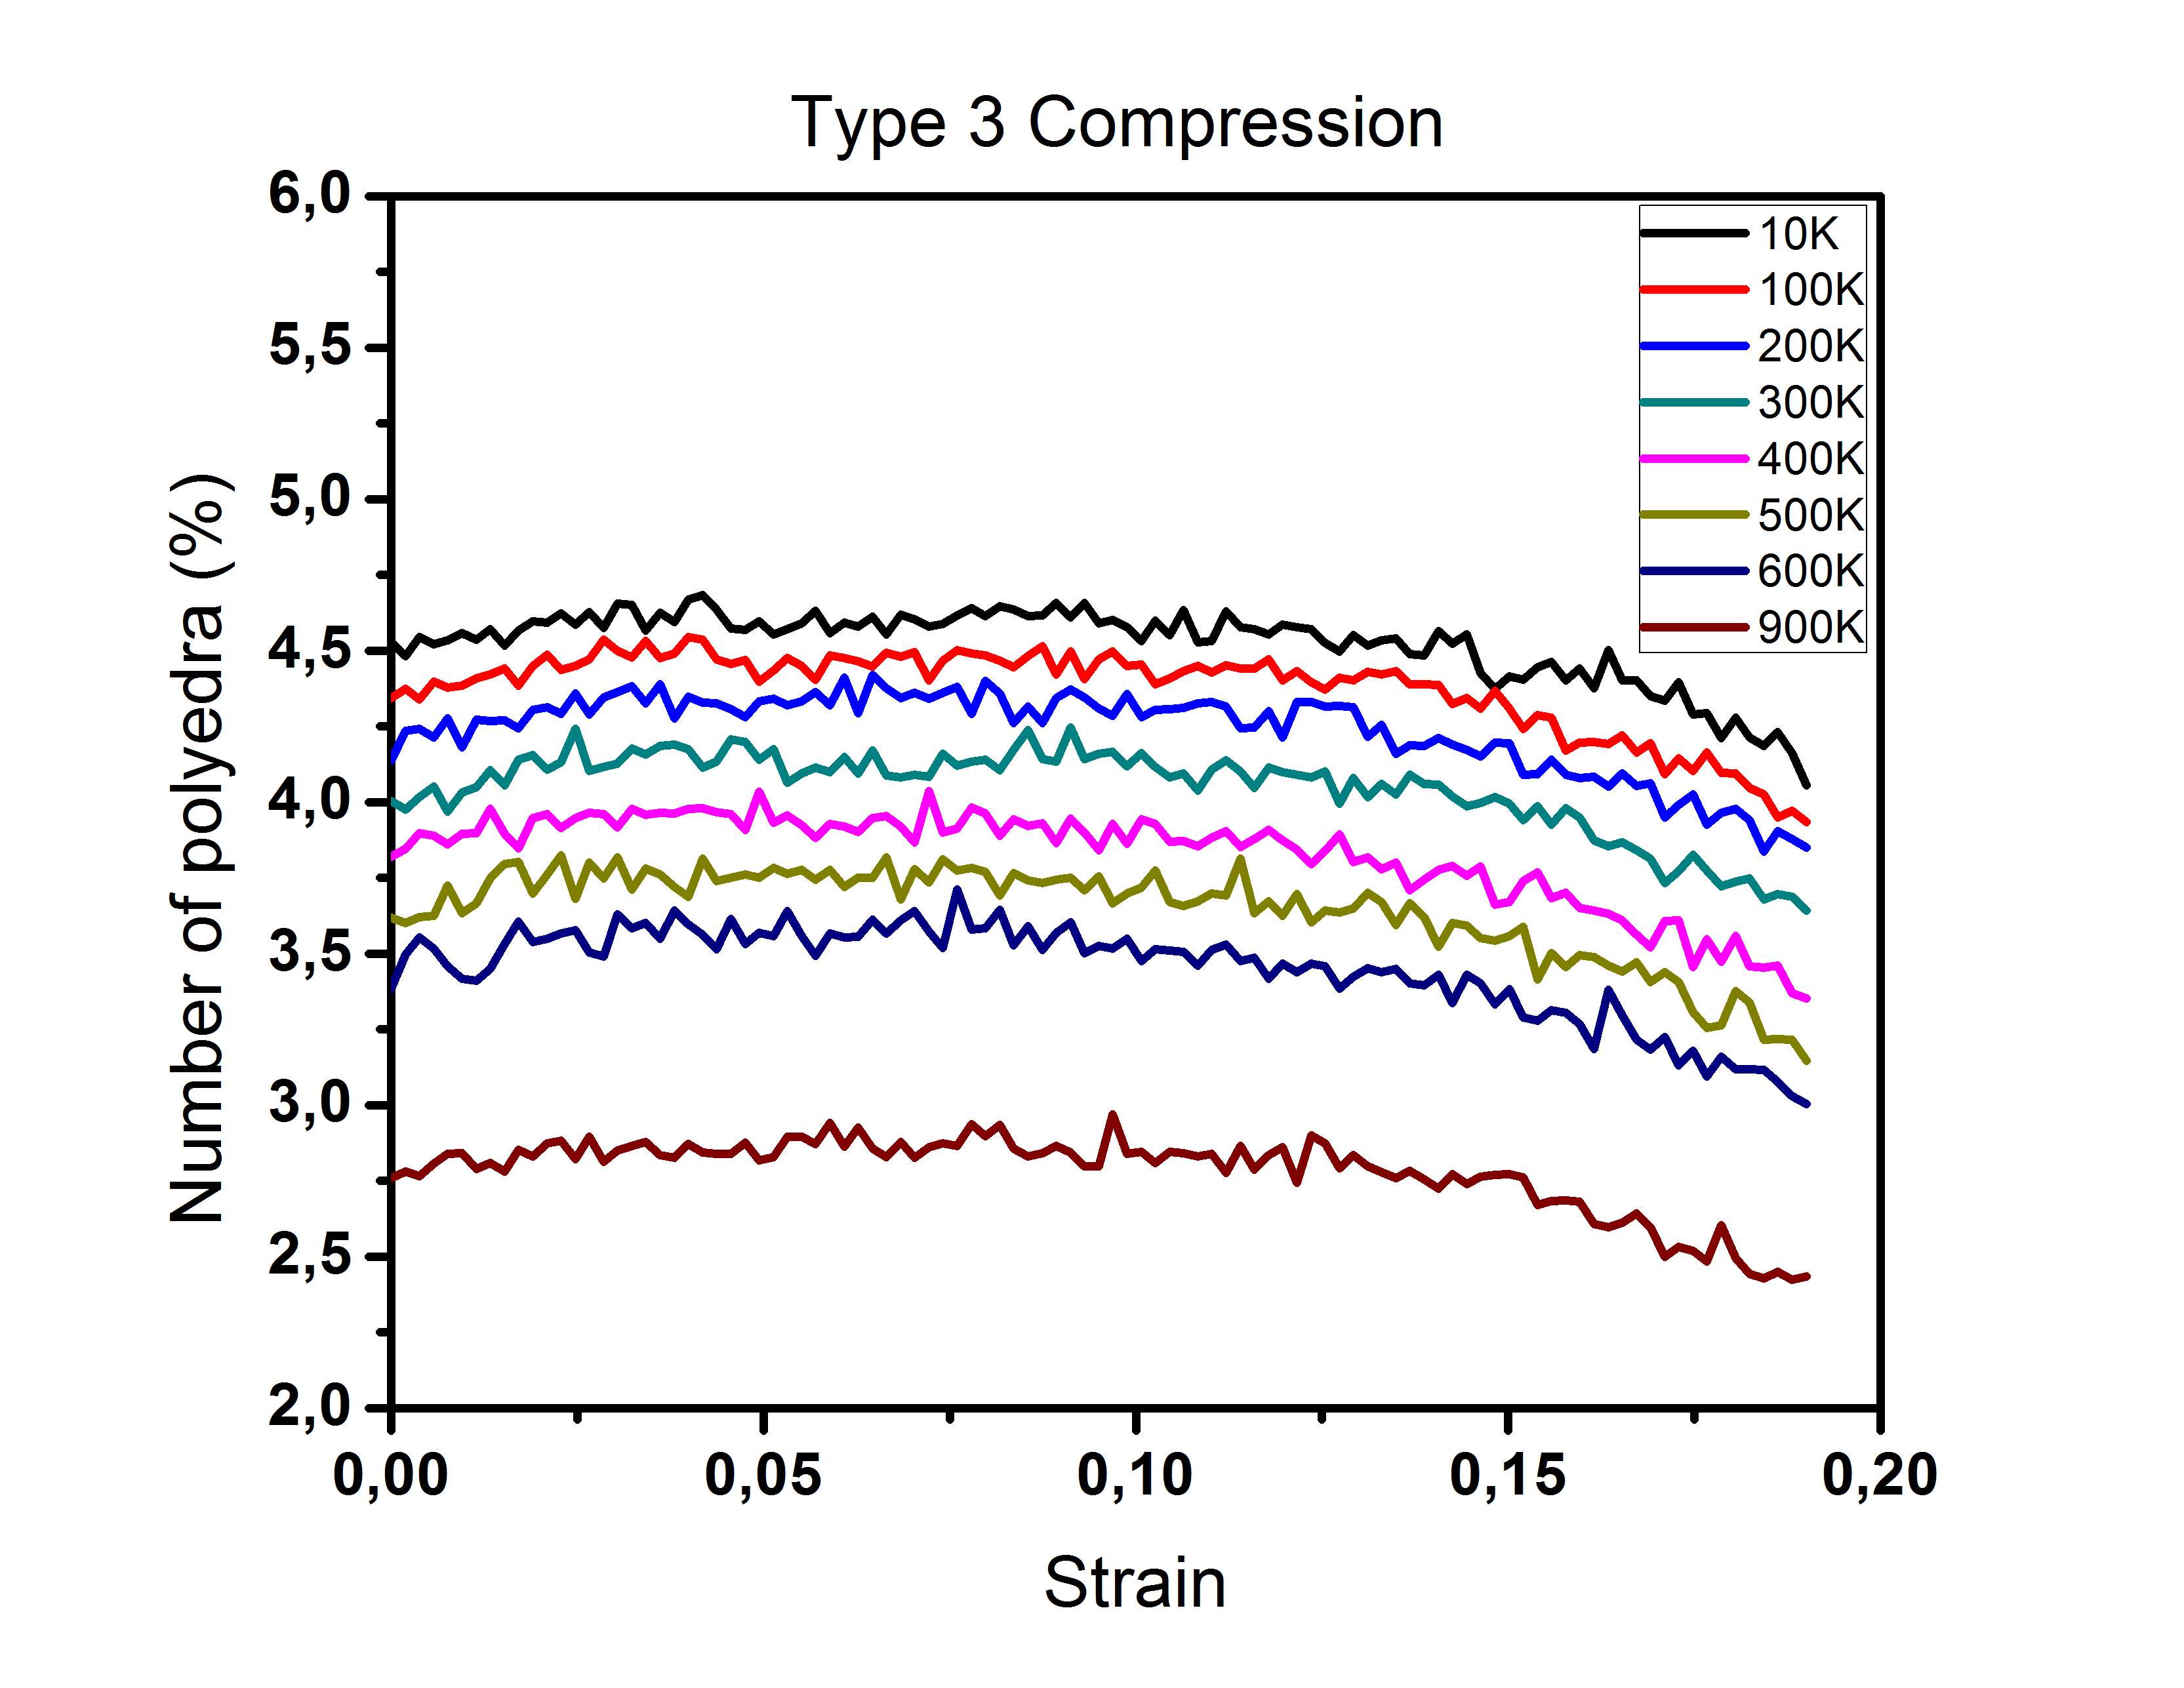
\includegraphics[width=8cm]{Figures/type3_COMP.png}
\caption{polyedros de voronoi tipo 3 vs. strain}
\end{figure}

\begin{figure}[H]
\centering
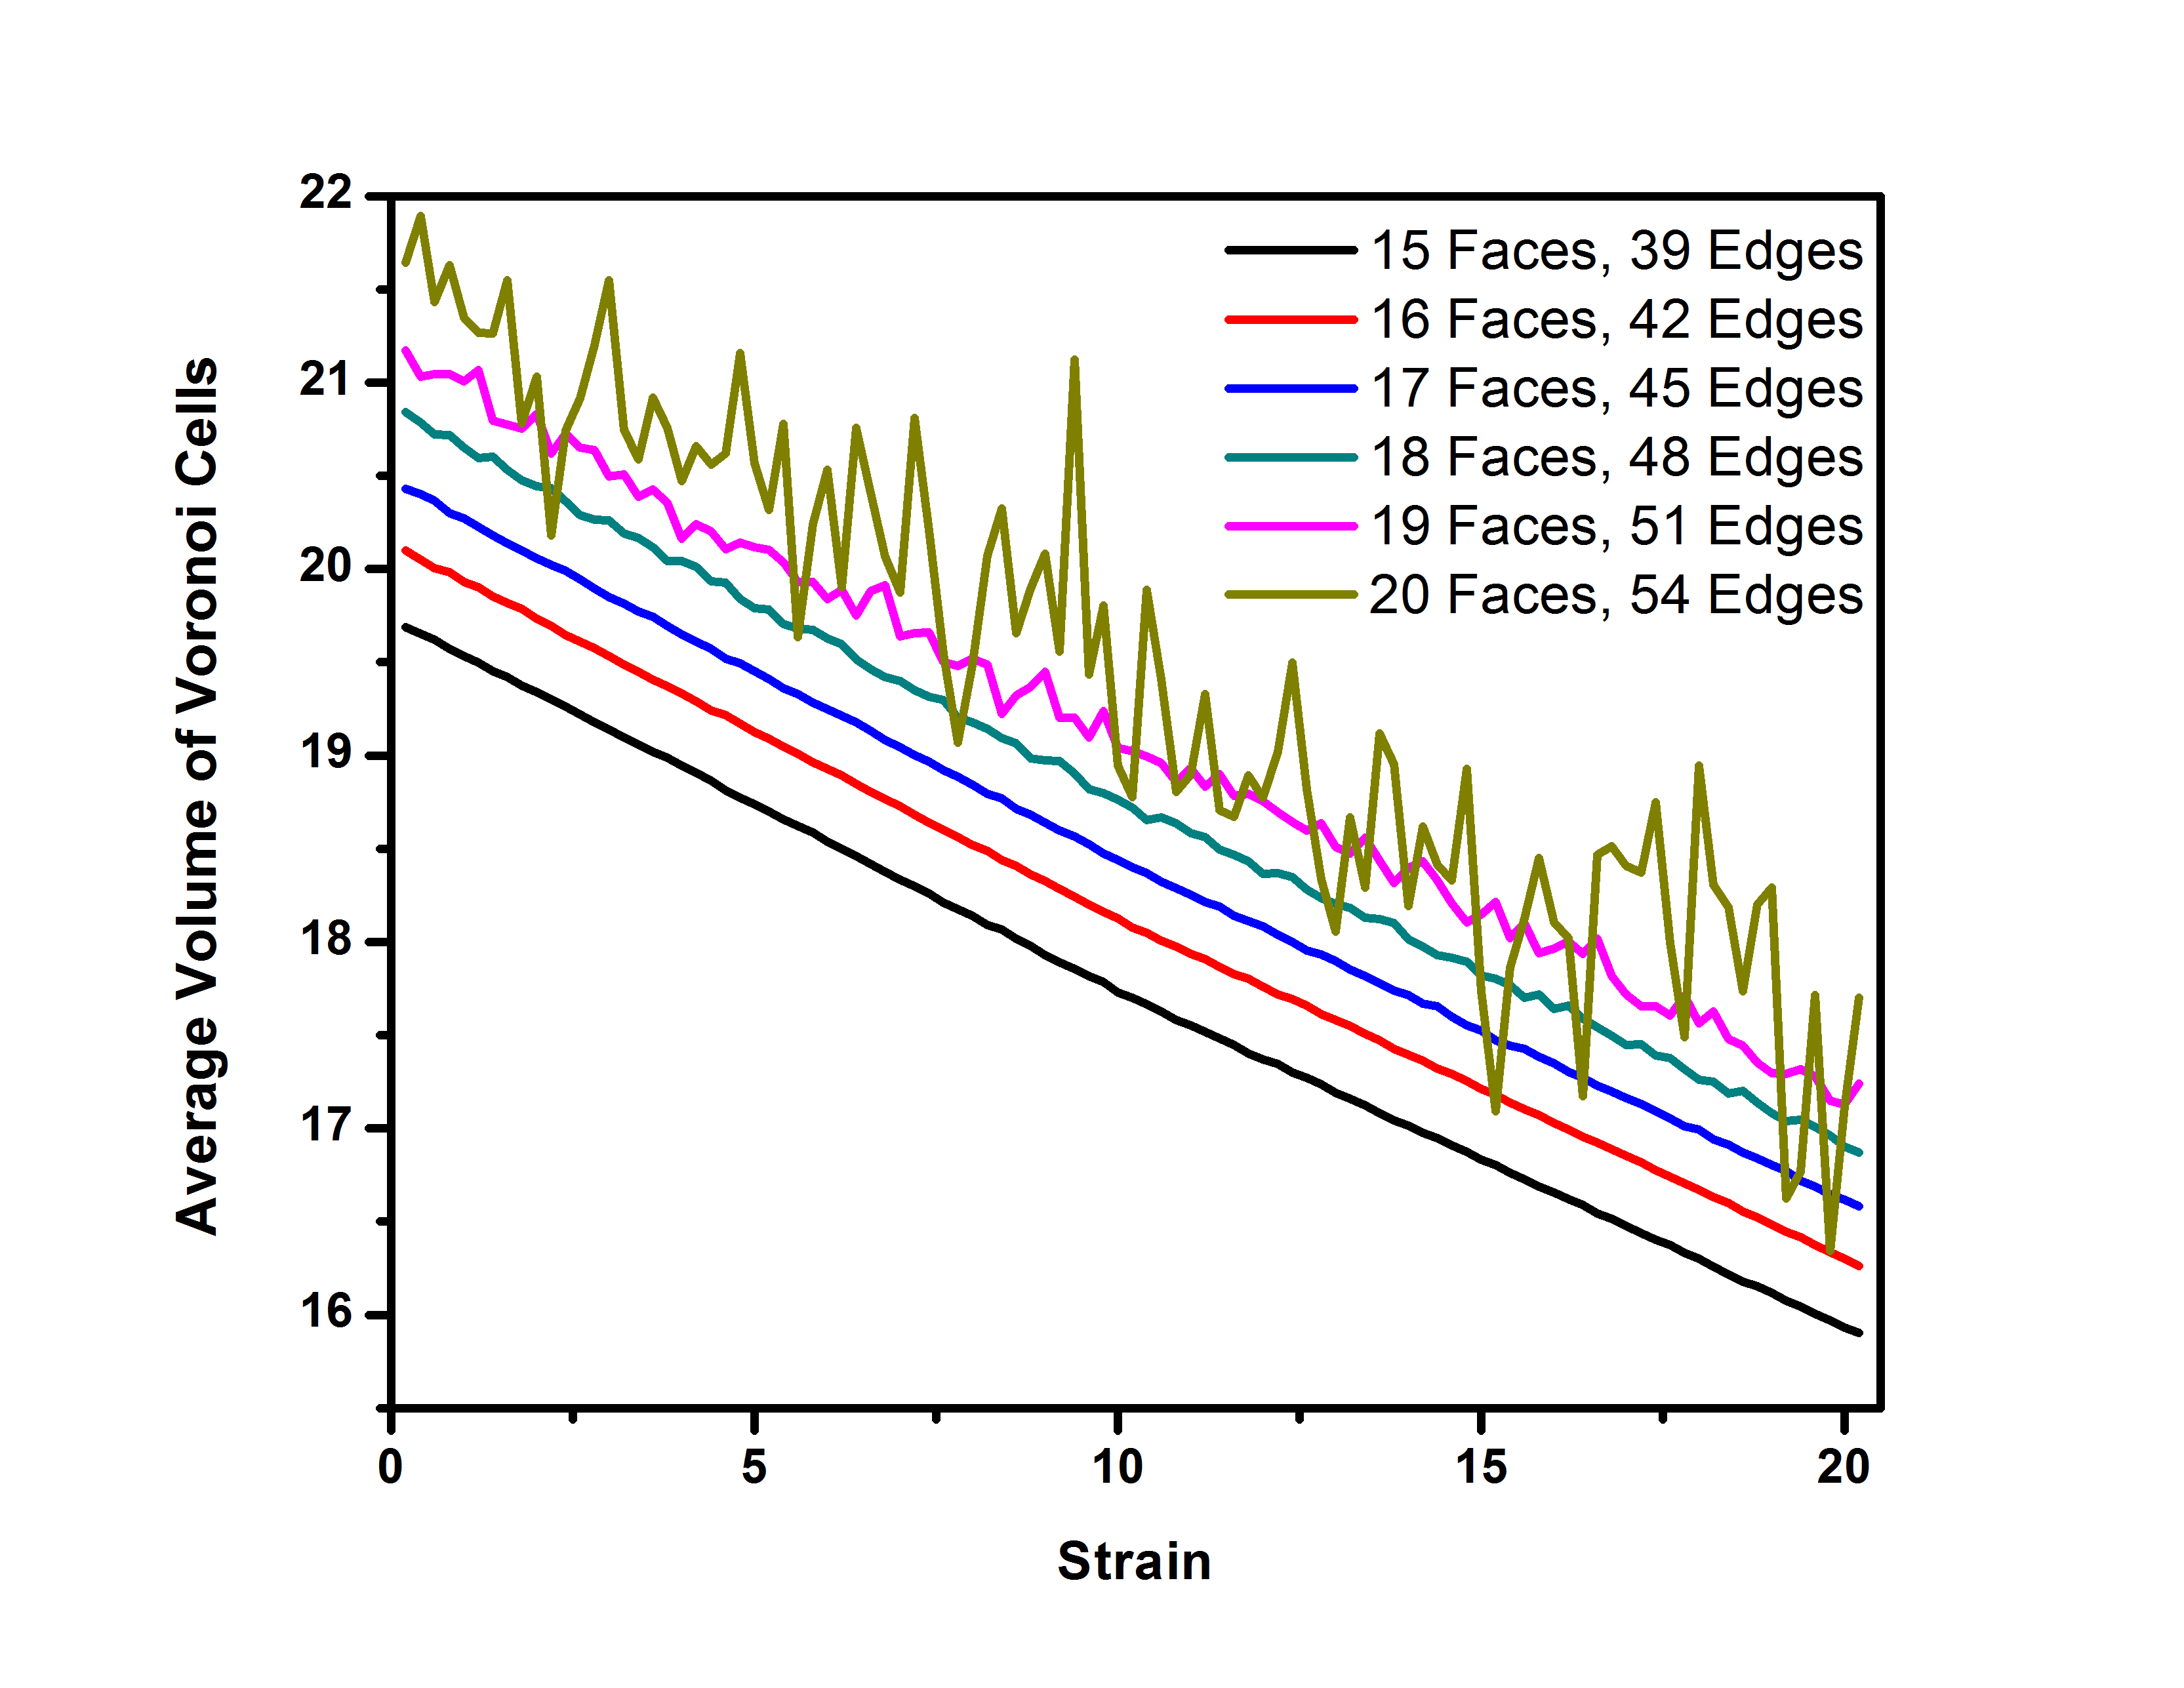
\includegraphics[width=8cm]{Figures/COMP_Vol_Step_A.png}
\caption{volumen promedio de voronoi cells (parte 1/2, temperatura desconocida)}
\end{figure}

\begin{figure}[H]
\centering
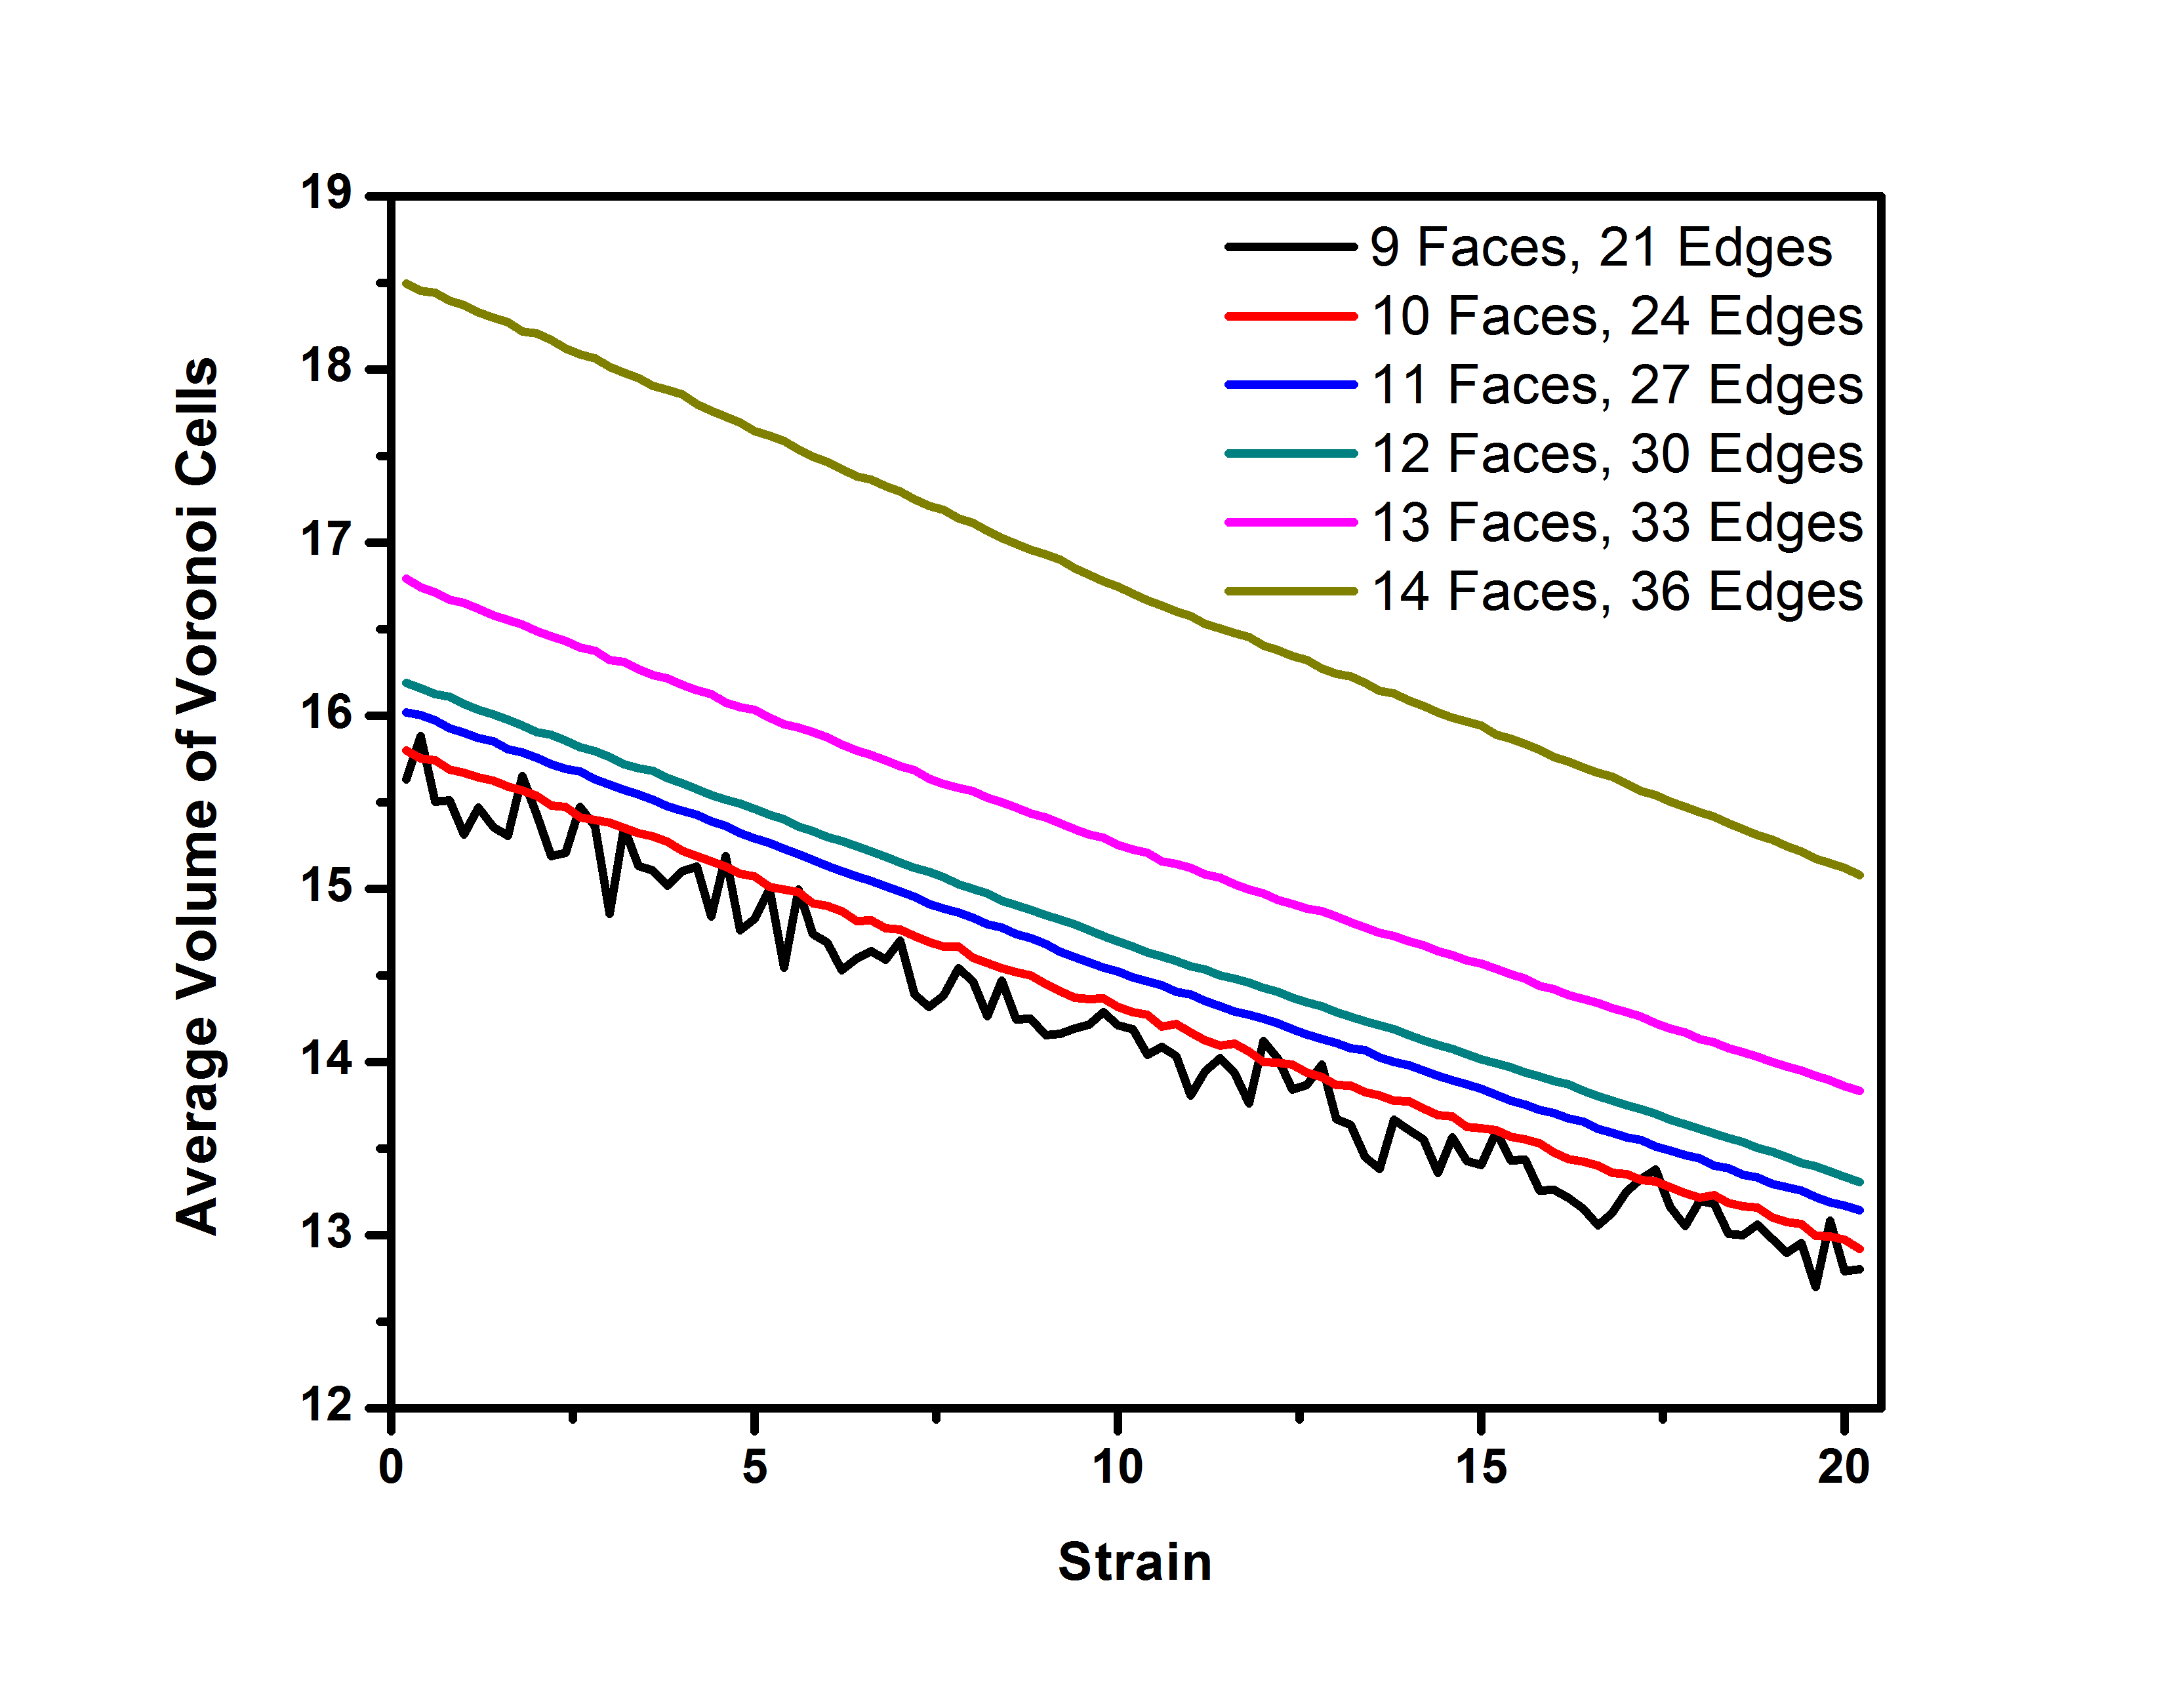
\includegraphics[width=8cm]{Figures/COMP_Vol_Step_B.png}
\caption{volumen promedio de voronoi cells (parte 2/2, temperatura desconocida)}
\end{figure}

\begin{figure}[H]
\centering
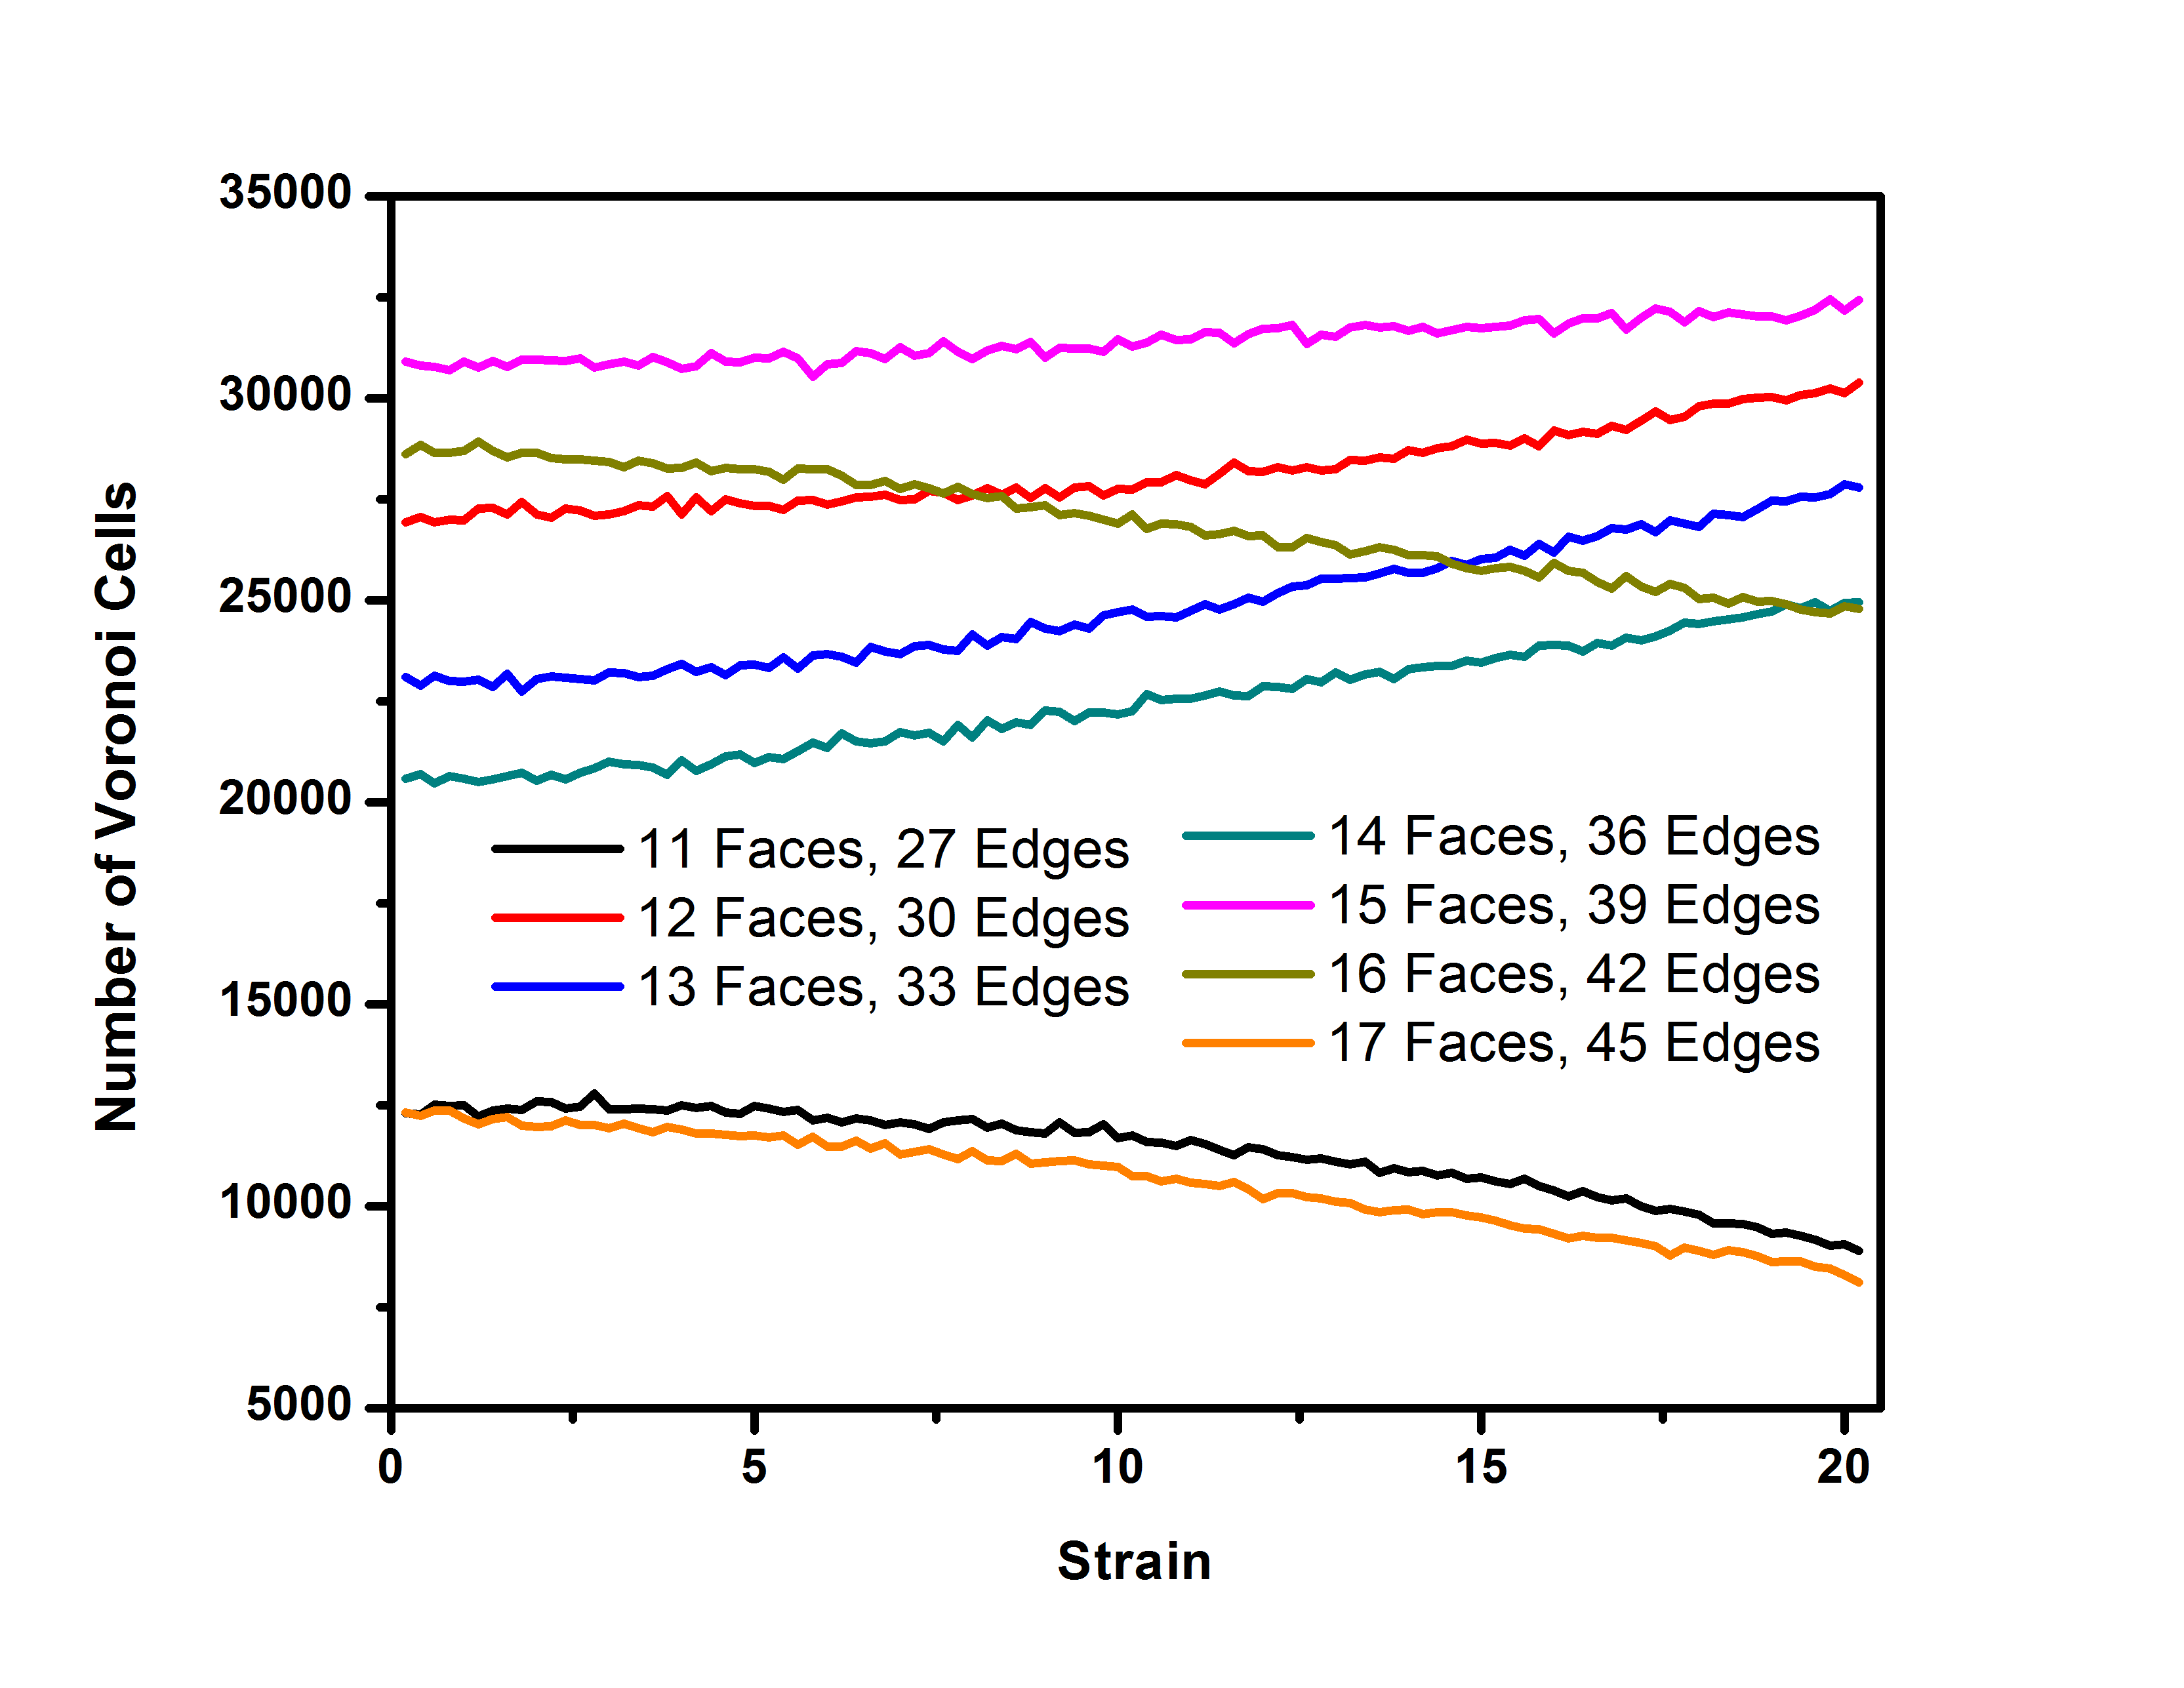
\includegraphics[width=8cm]{Figures/COMP_Num_Step.png}
\caption{numero celdas de voronoi (temperatura desconocida)}
\end{figure}

\begin{figure}[H]
\centering
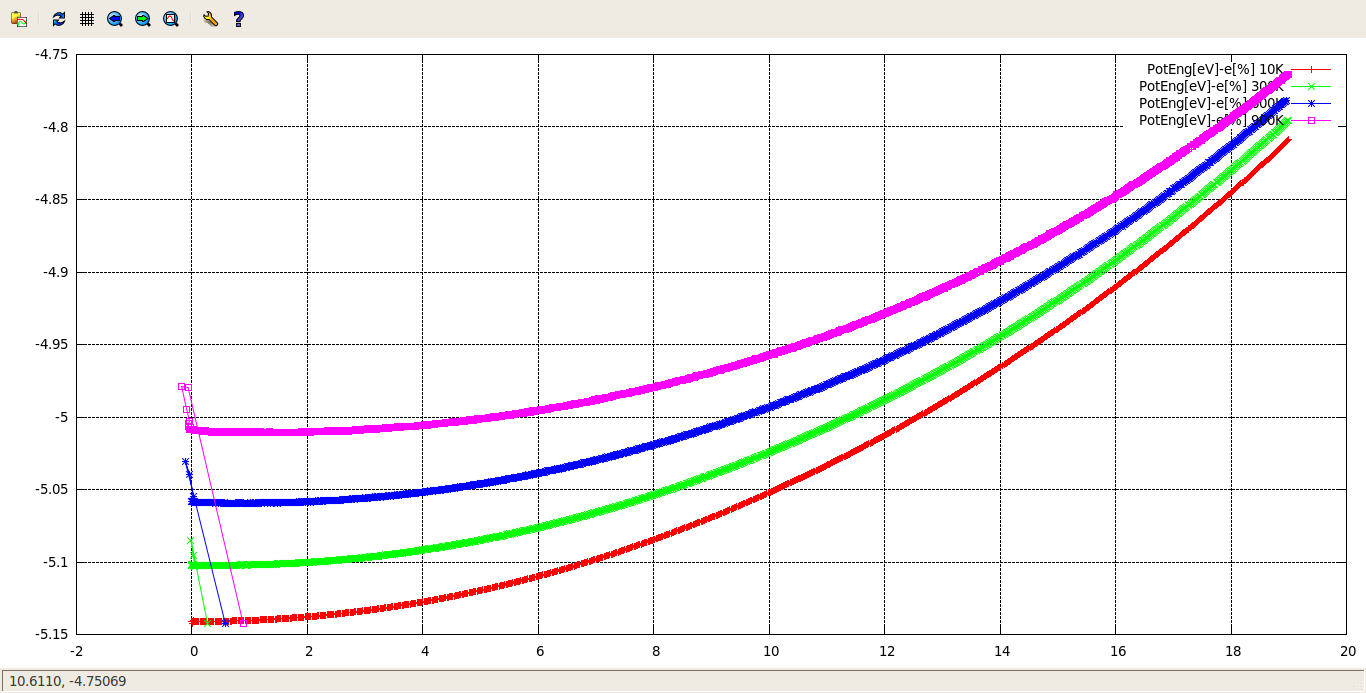
\includegraphics[width=8cm]{Figures/EngPot_COMP.png}
\caption{Energia potencial}
\end{figure}

\begin{figure}[H]
\centering
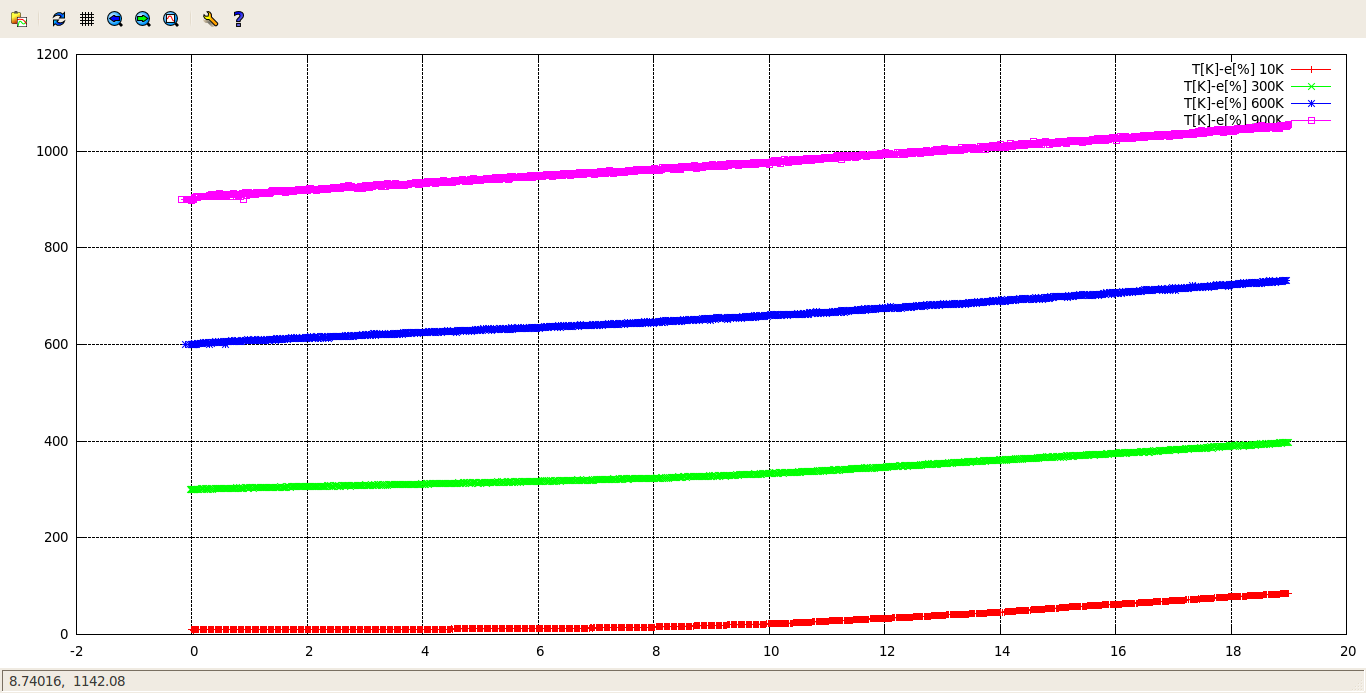
\includegraphics[width=8cm]{Figures/Temp_COMP.png}
\caption{Temperatura}
\end{figure}


%
%	Traccion
%

\subsection{Traccion}

\begin{figure}[H]
\centering
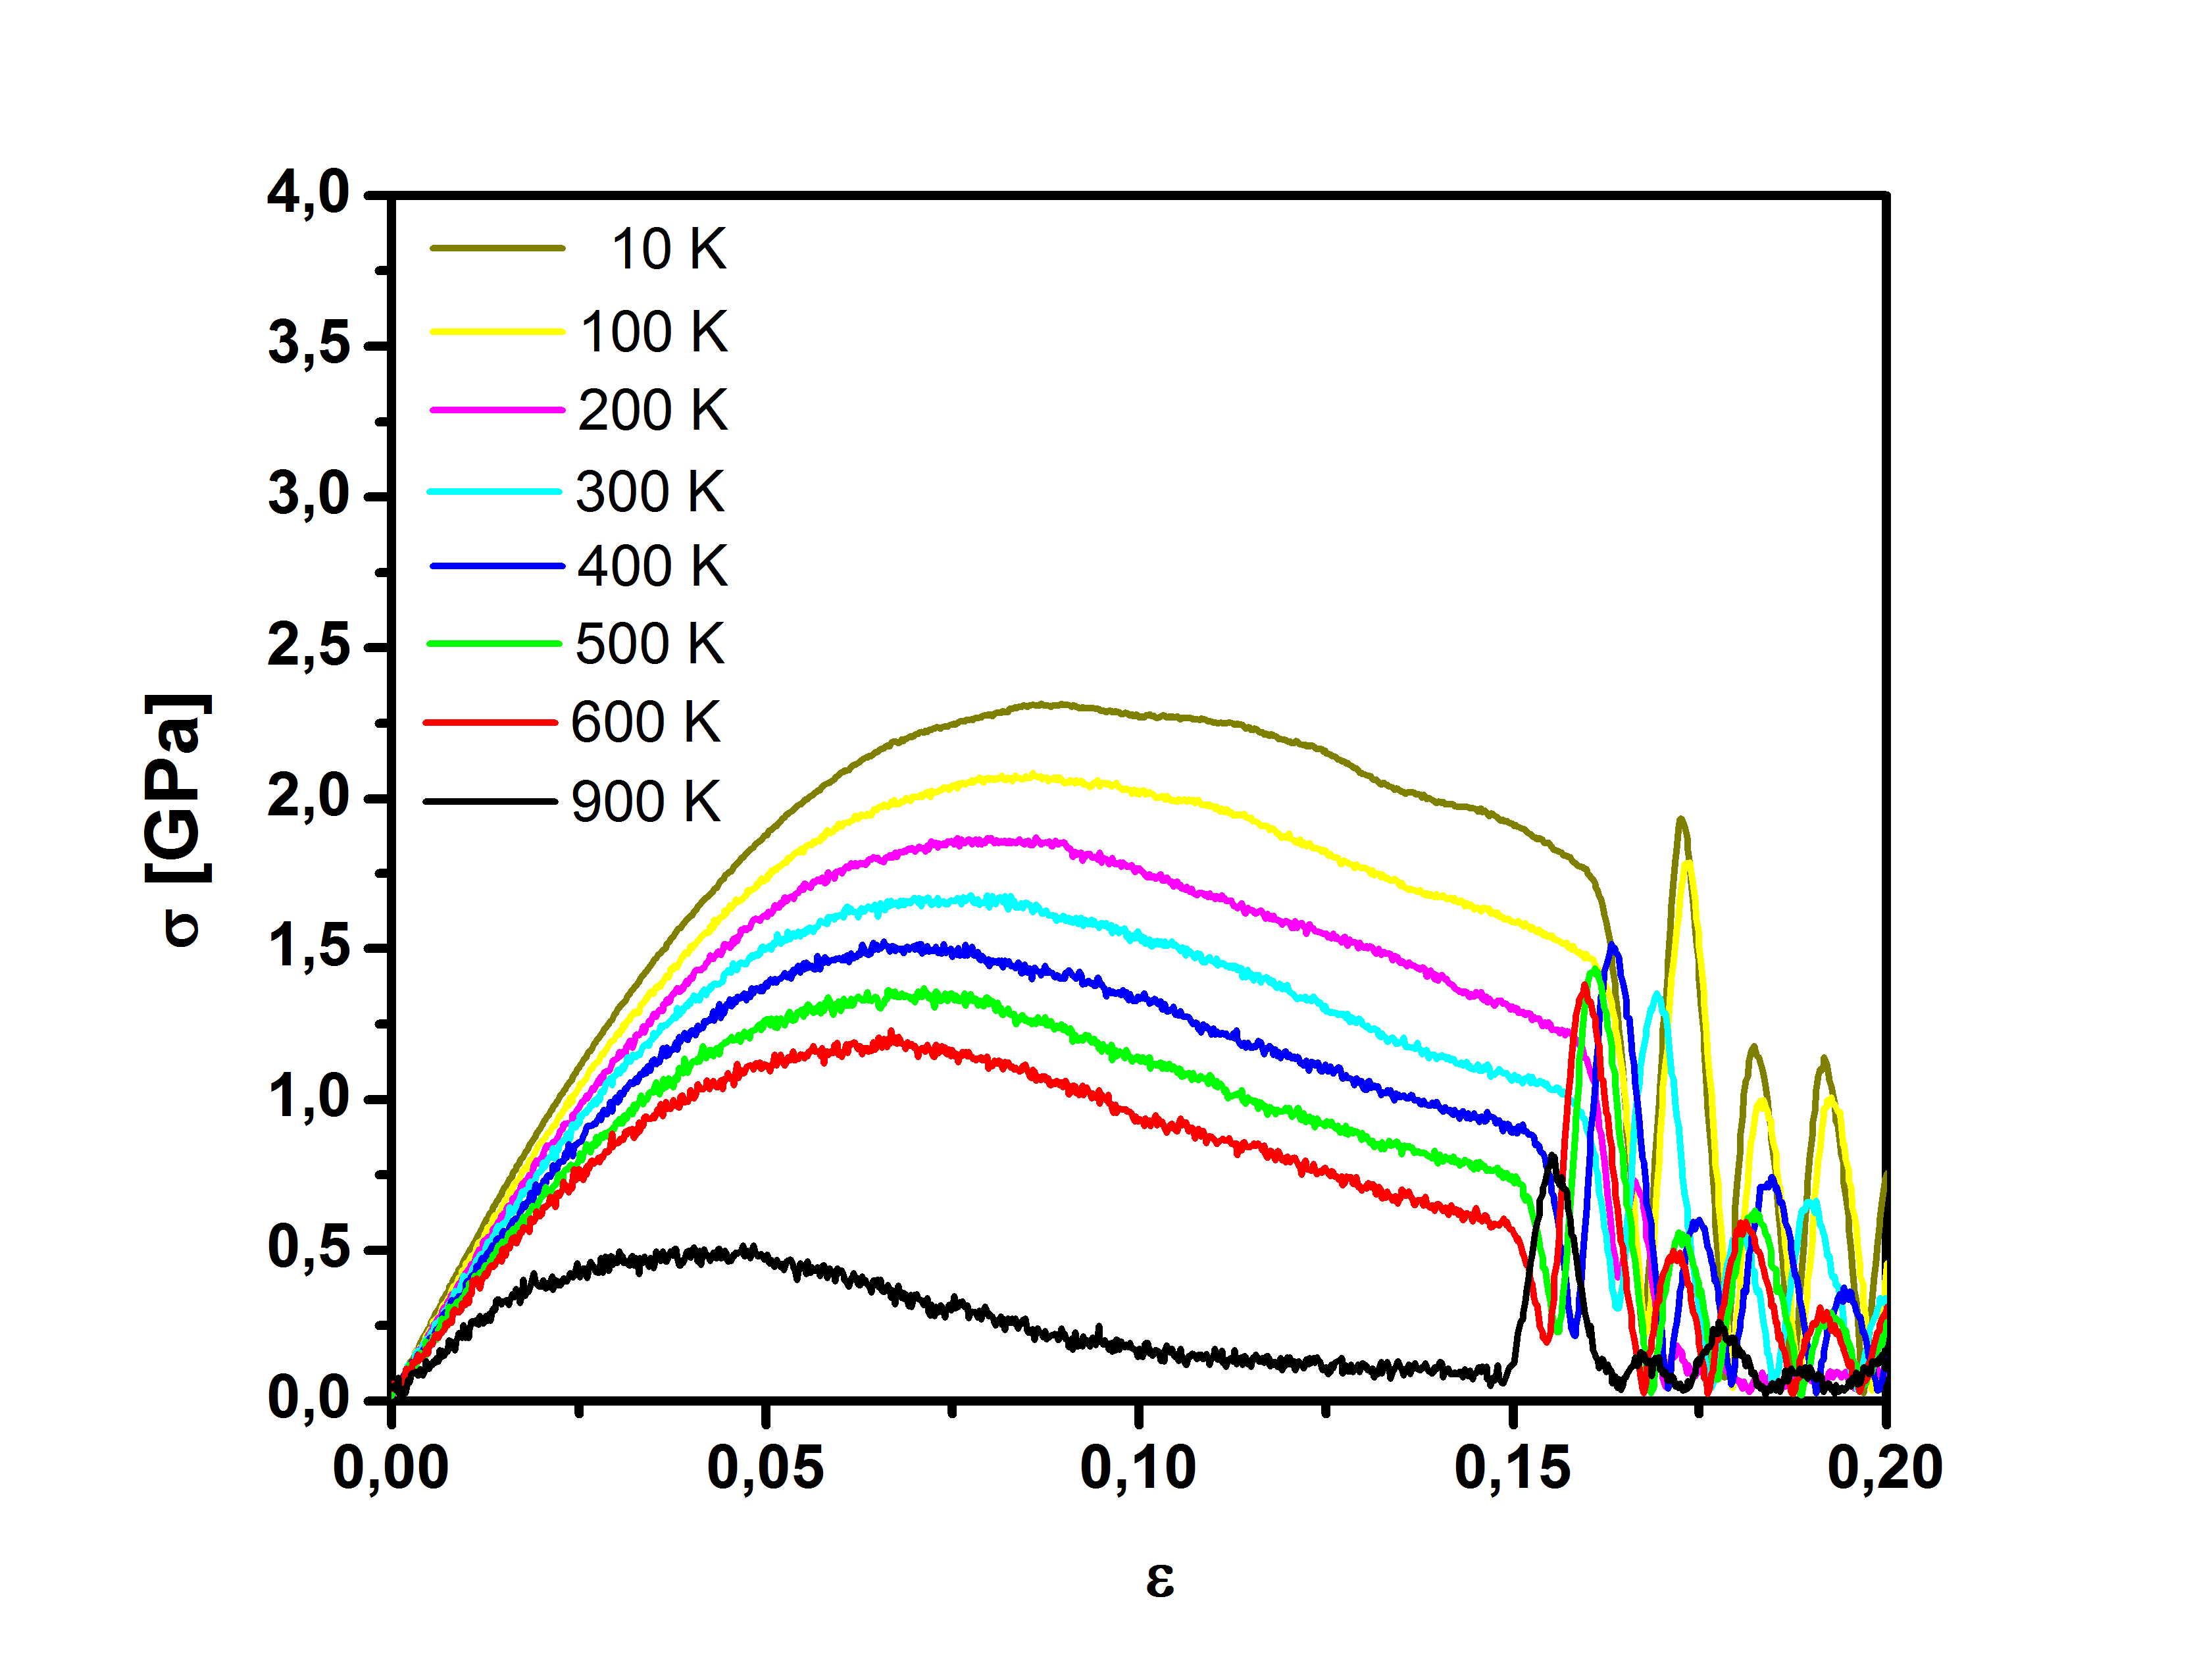
\includegraphics[width=8cm]{Figures/stress_strain_TEN.png}
\caption{Von Mises vs. strain}
\end{figure}

\begin{figure}[H]
\centering
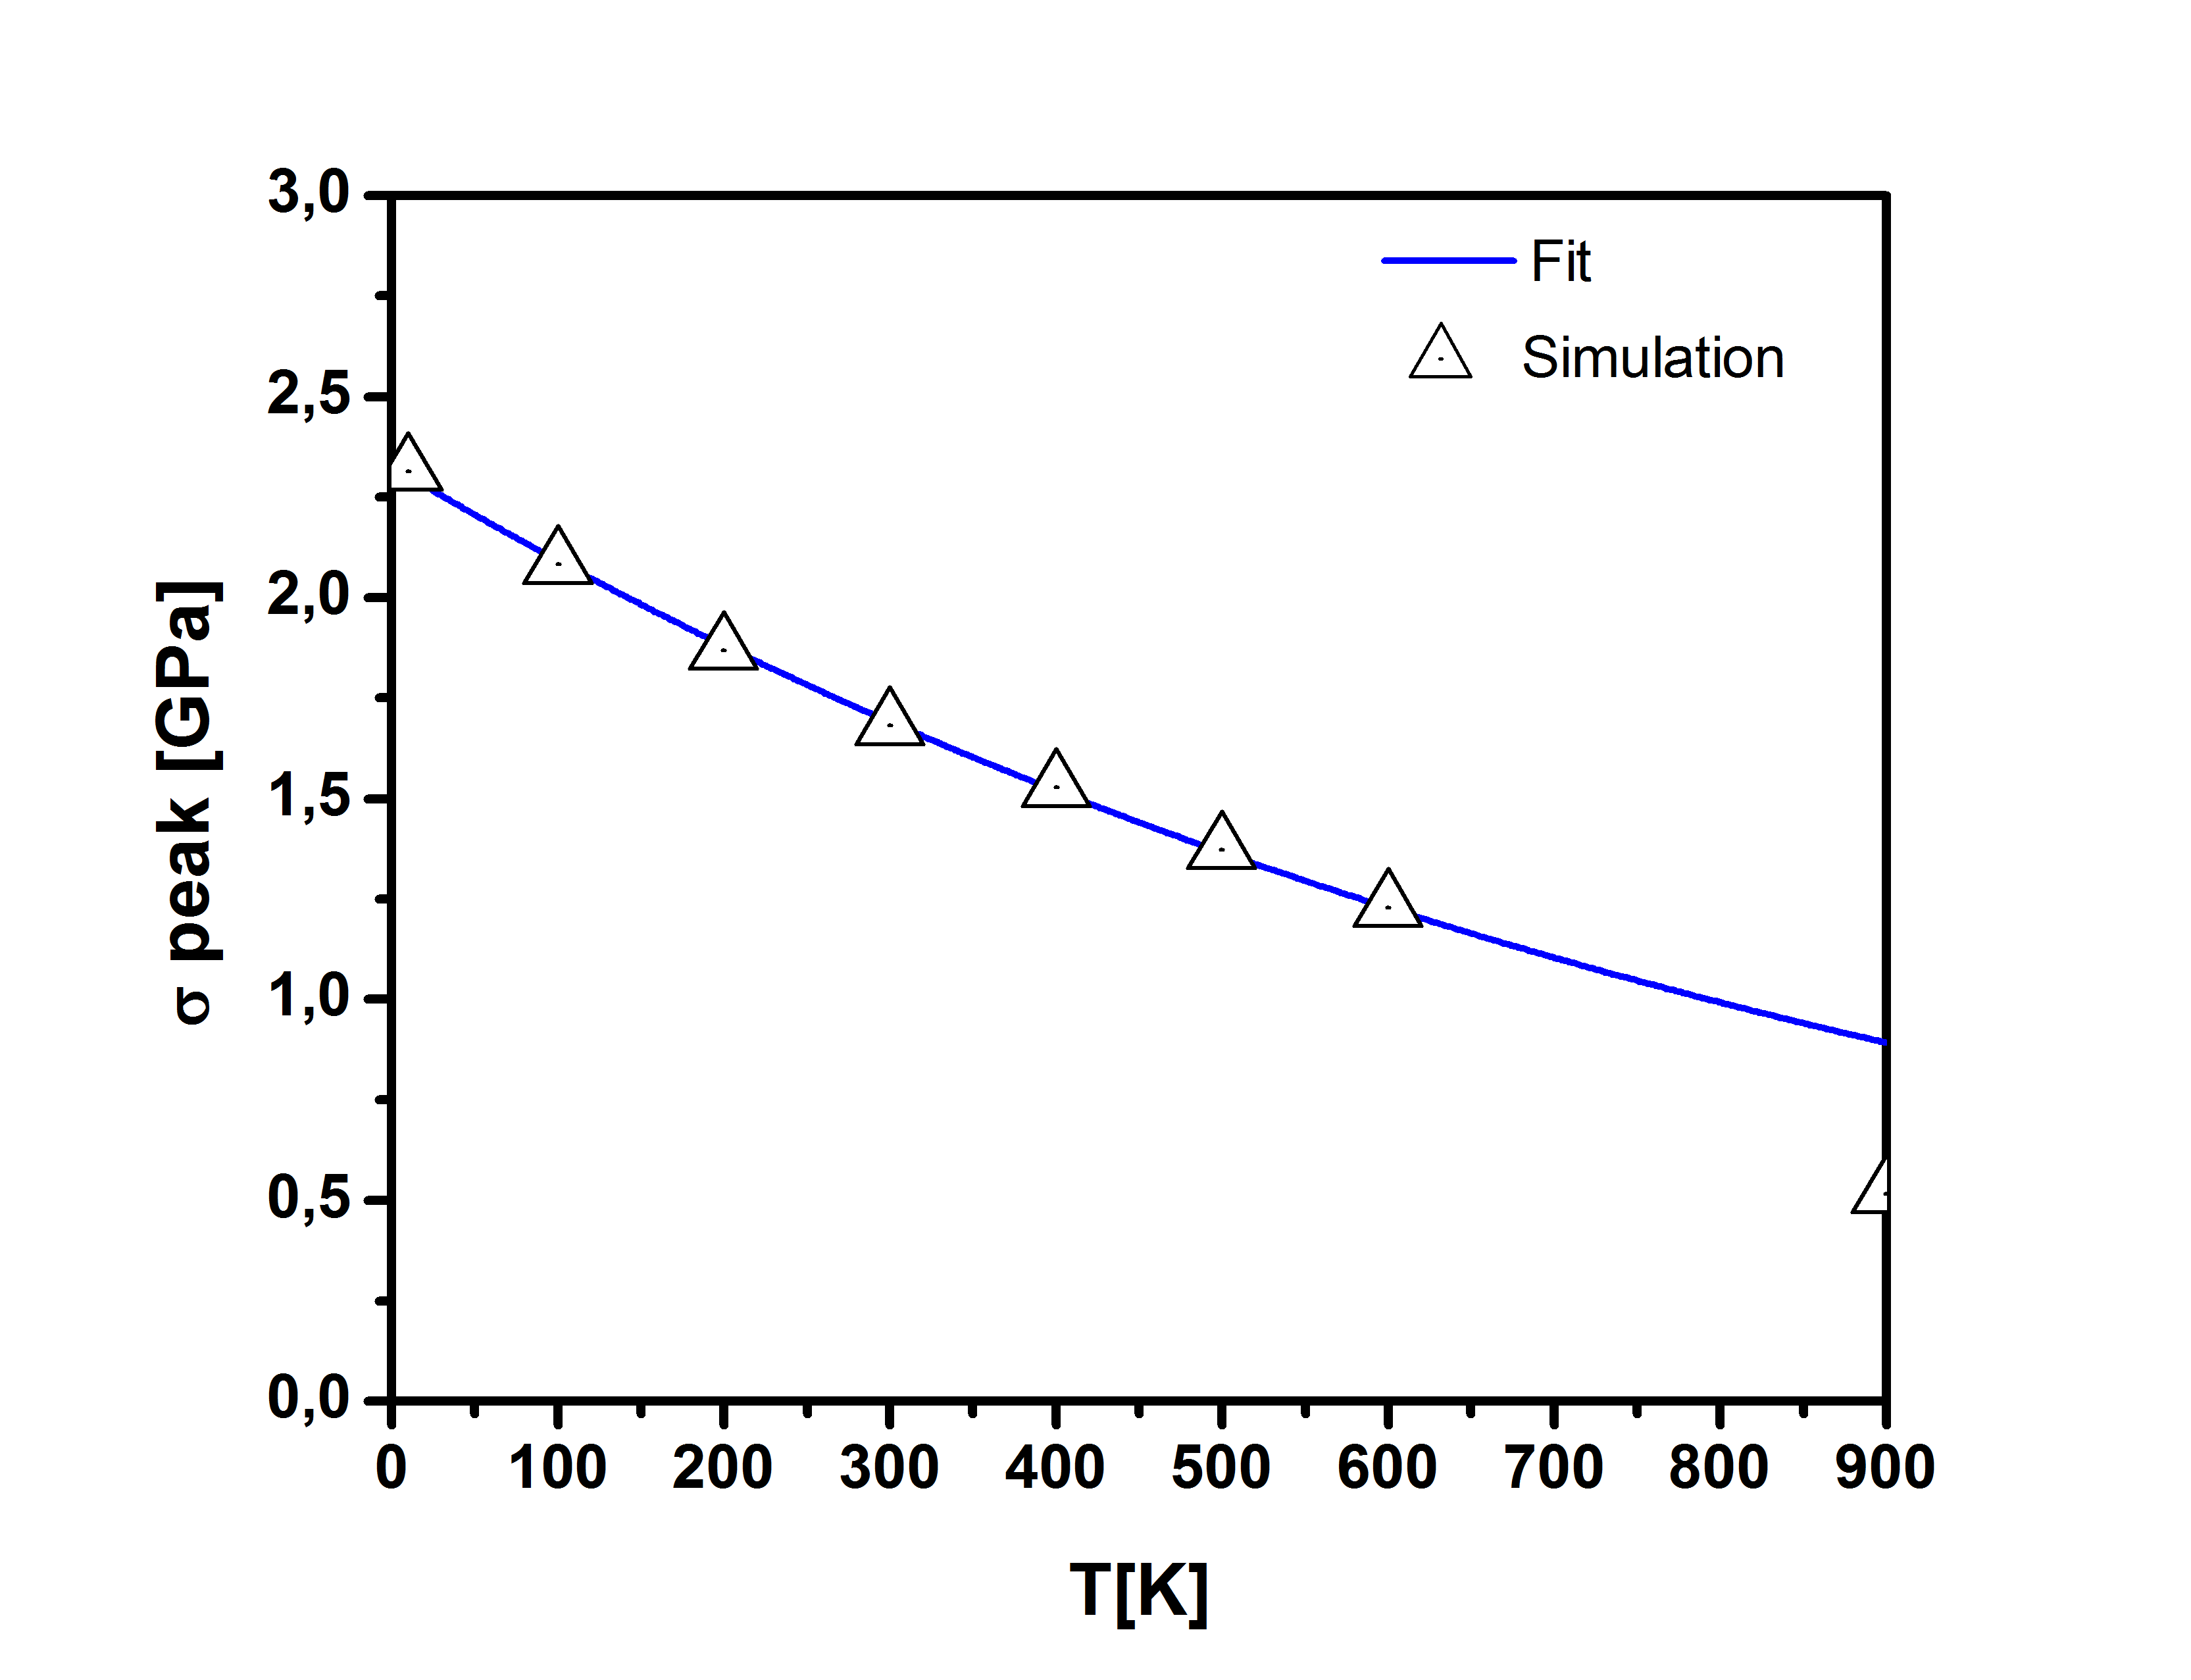
\includegraphics[width=8cm]{Figures/peakstress_T_TEN.png}
\caption{Von Mises maximo vs. Temperatura}
\end{figure}

\begin{figure}[H]
\centering
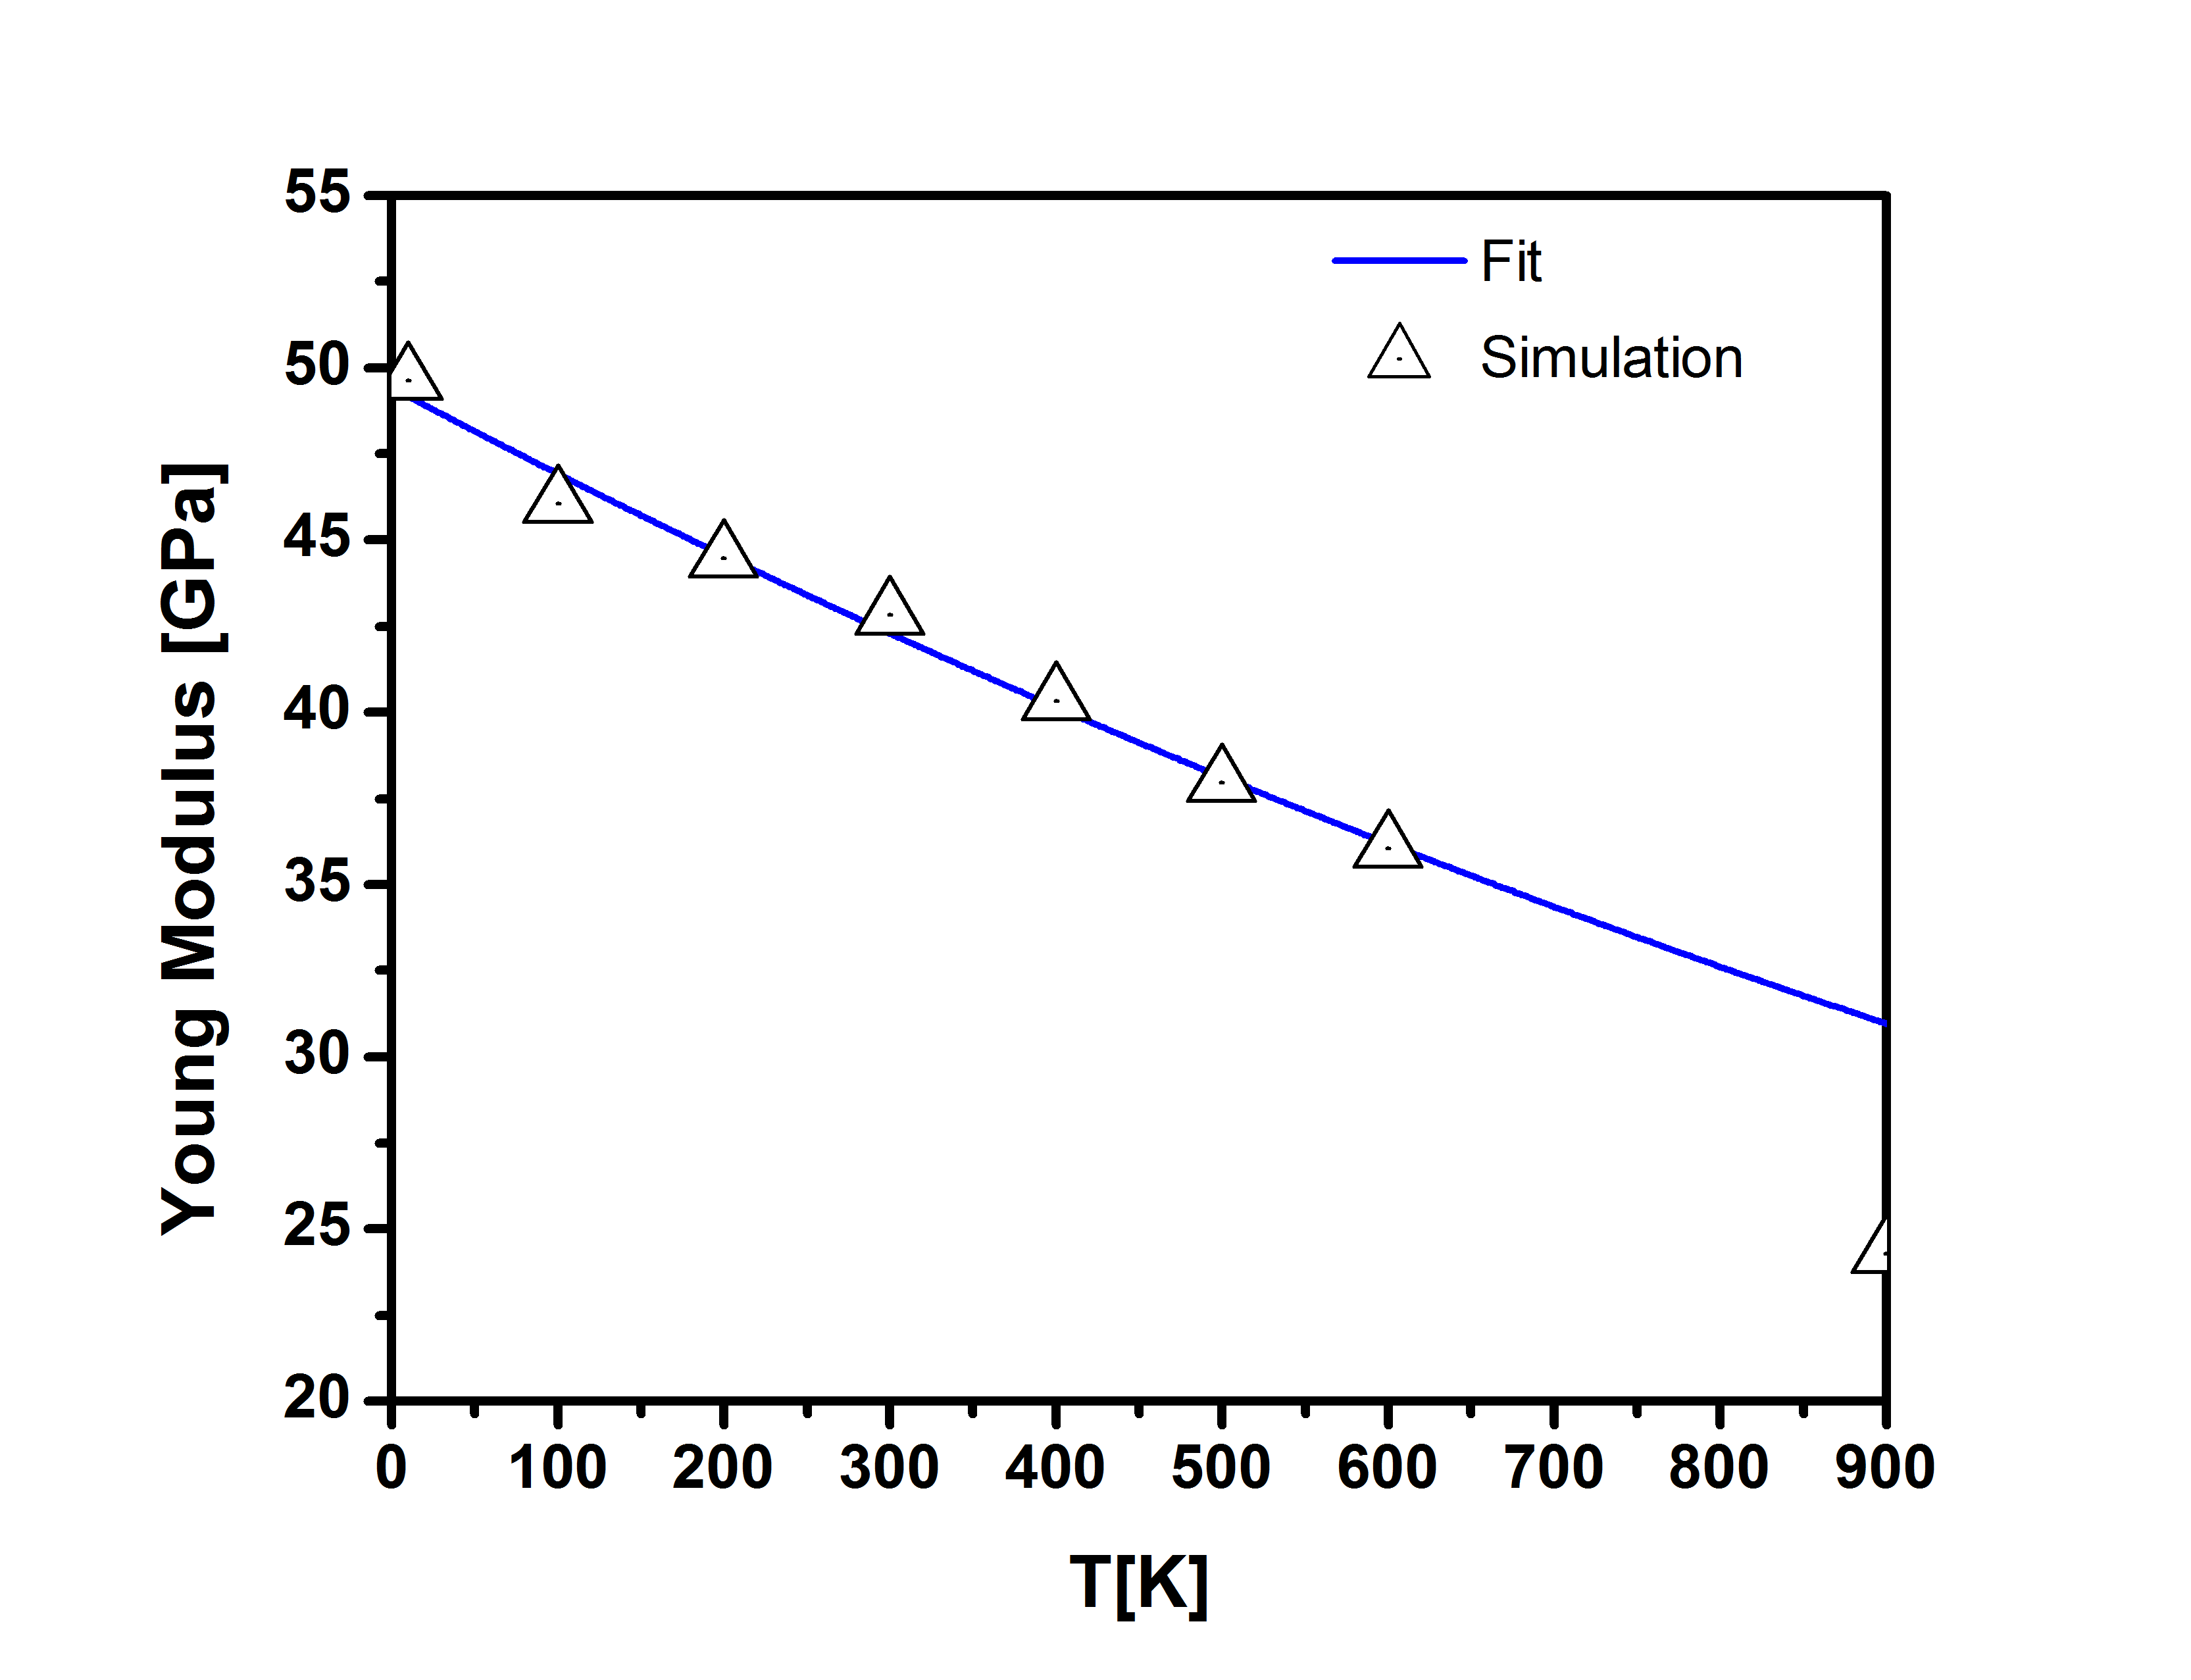
\includegraphics[width=8cm]{Figures/young_T_TEN.png}
\caption{Modulo Young vs. Temperatura}
\end{figure}

\begin{figure}[H]
\centering
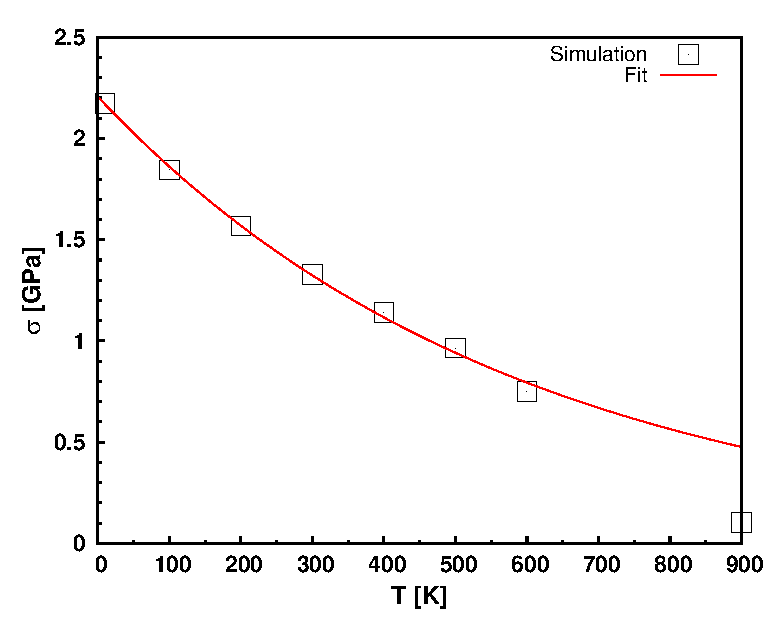
\includegraphics[width=8cm]{Figures/12stress_T_TENS.eps}
\caption{Von Mises a strain 12\% vs. Temperatura}
\end{figure}

\begin{figure}[H]
\centering
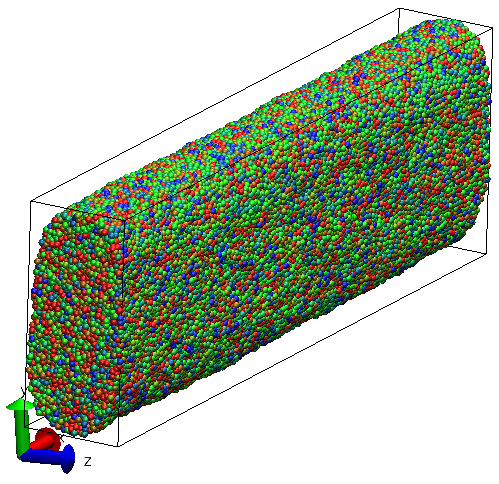
\includegraphics[width=8cm]{Figures/900libresTen.png}
\caption{Muestra a 300K cond. de frontera libres strain 20\%}
\end{figure}

\begin{figure}[H]
\centering
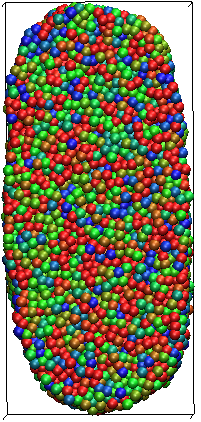
\includegraphics[width=2cm]{Figures/crossa.png}
\caption{Seccion transversal (cond. frontera libres) en el extremo de la muestra}
\end{figure}

\begin{figure}[H]
\centering
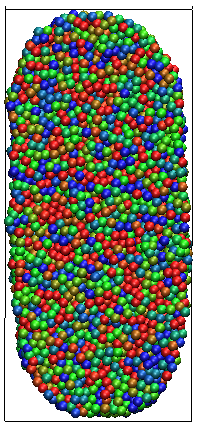
\includegraphics[width=2cm]{Figures/crossb.png}
\caption{Seccion transversal (cond. frontera libres) en el centro de la muestra}
\end{figure}

\begin{figure}[H]
\centering
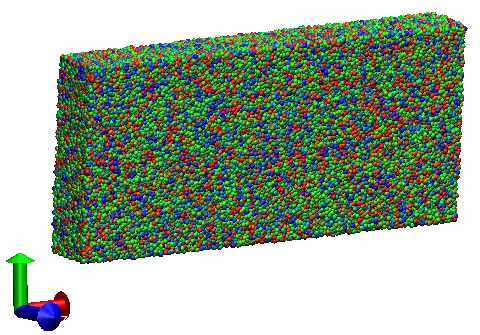
\includegraphics[width=8cm]{Figures/All_300K_6pstrain_sacale100-280_Trac.png}
\caption{Muestra a 300K cond. de frontera periodicas, 6\% strain, escala de colores 100-280 GPa}
\end{figure}

\begin{figure}[H]
\centering
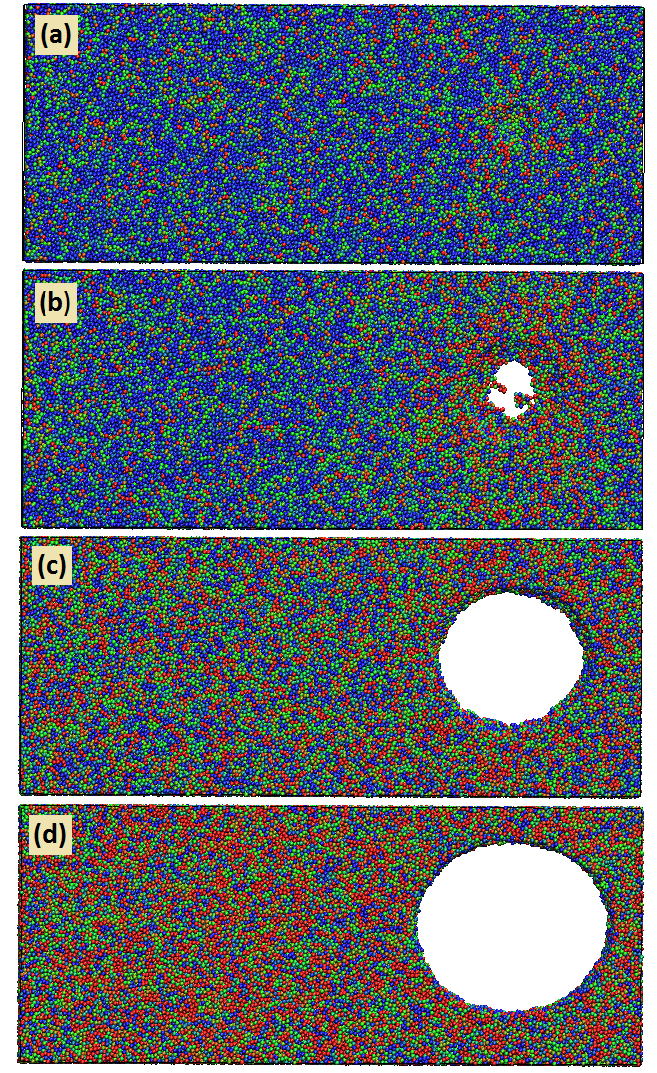
\includegraphics[width=8cm]{Figures/void_sequence.png}
\caption{Secuencia de formacion de void a 900K (strains 13.8, 14.2, 14.6, 15)}
\end{figure}

\begin{figure}[H]
\centering
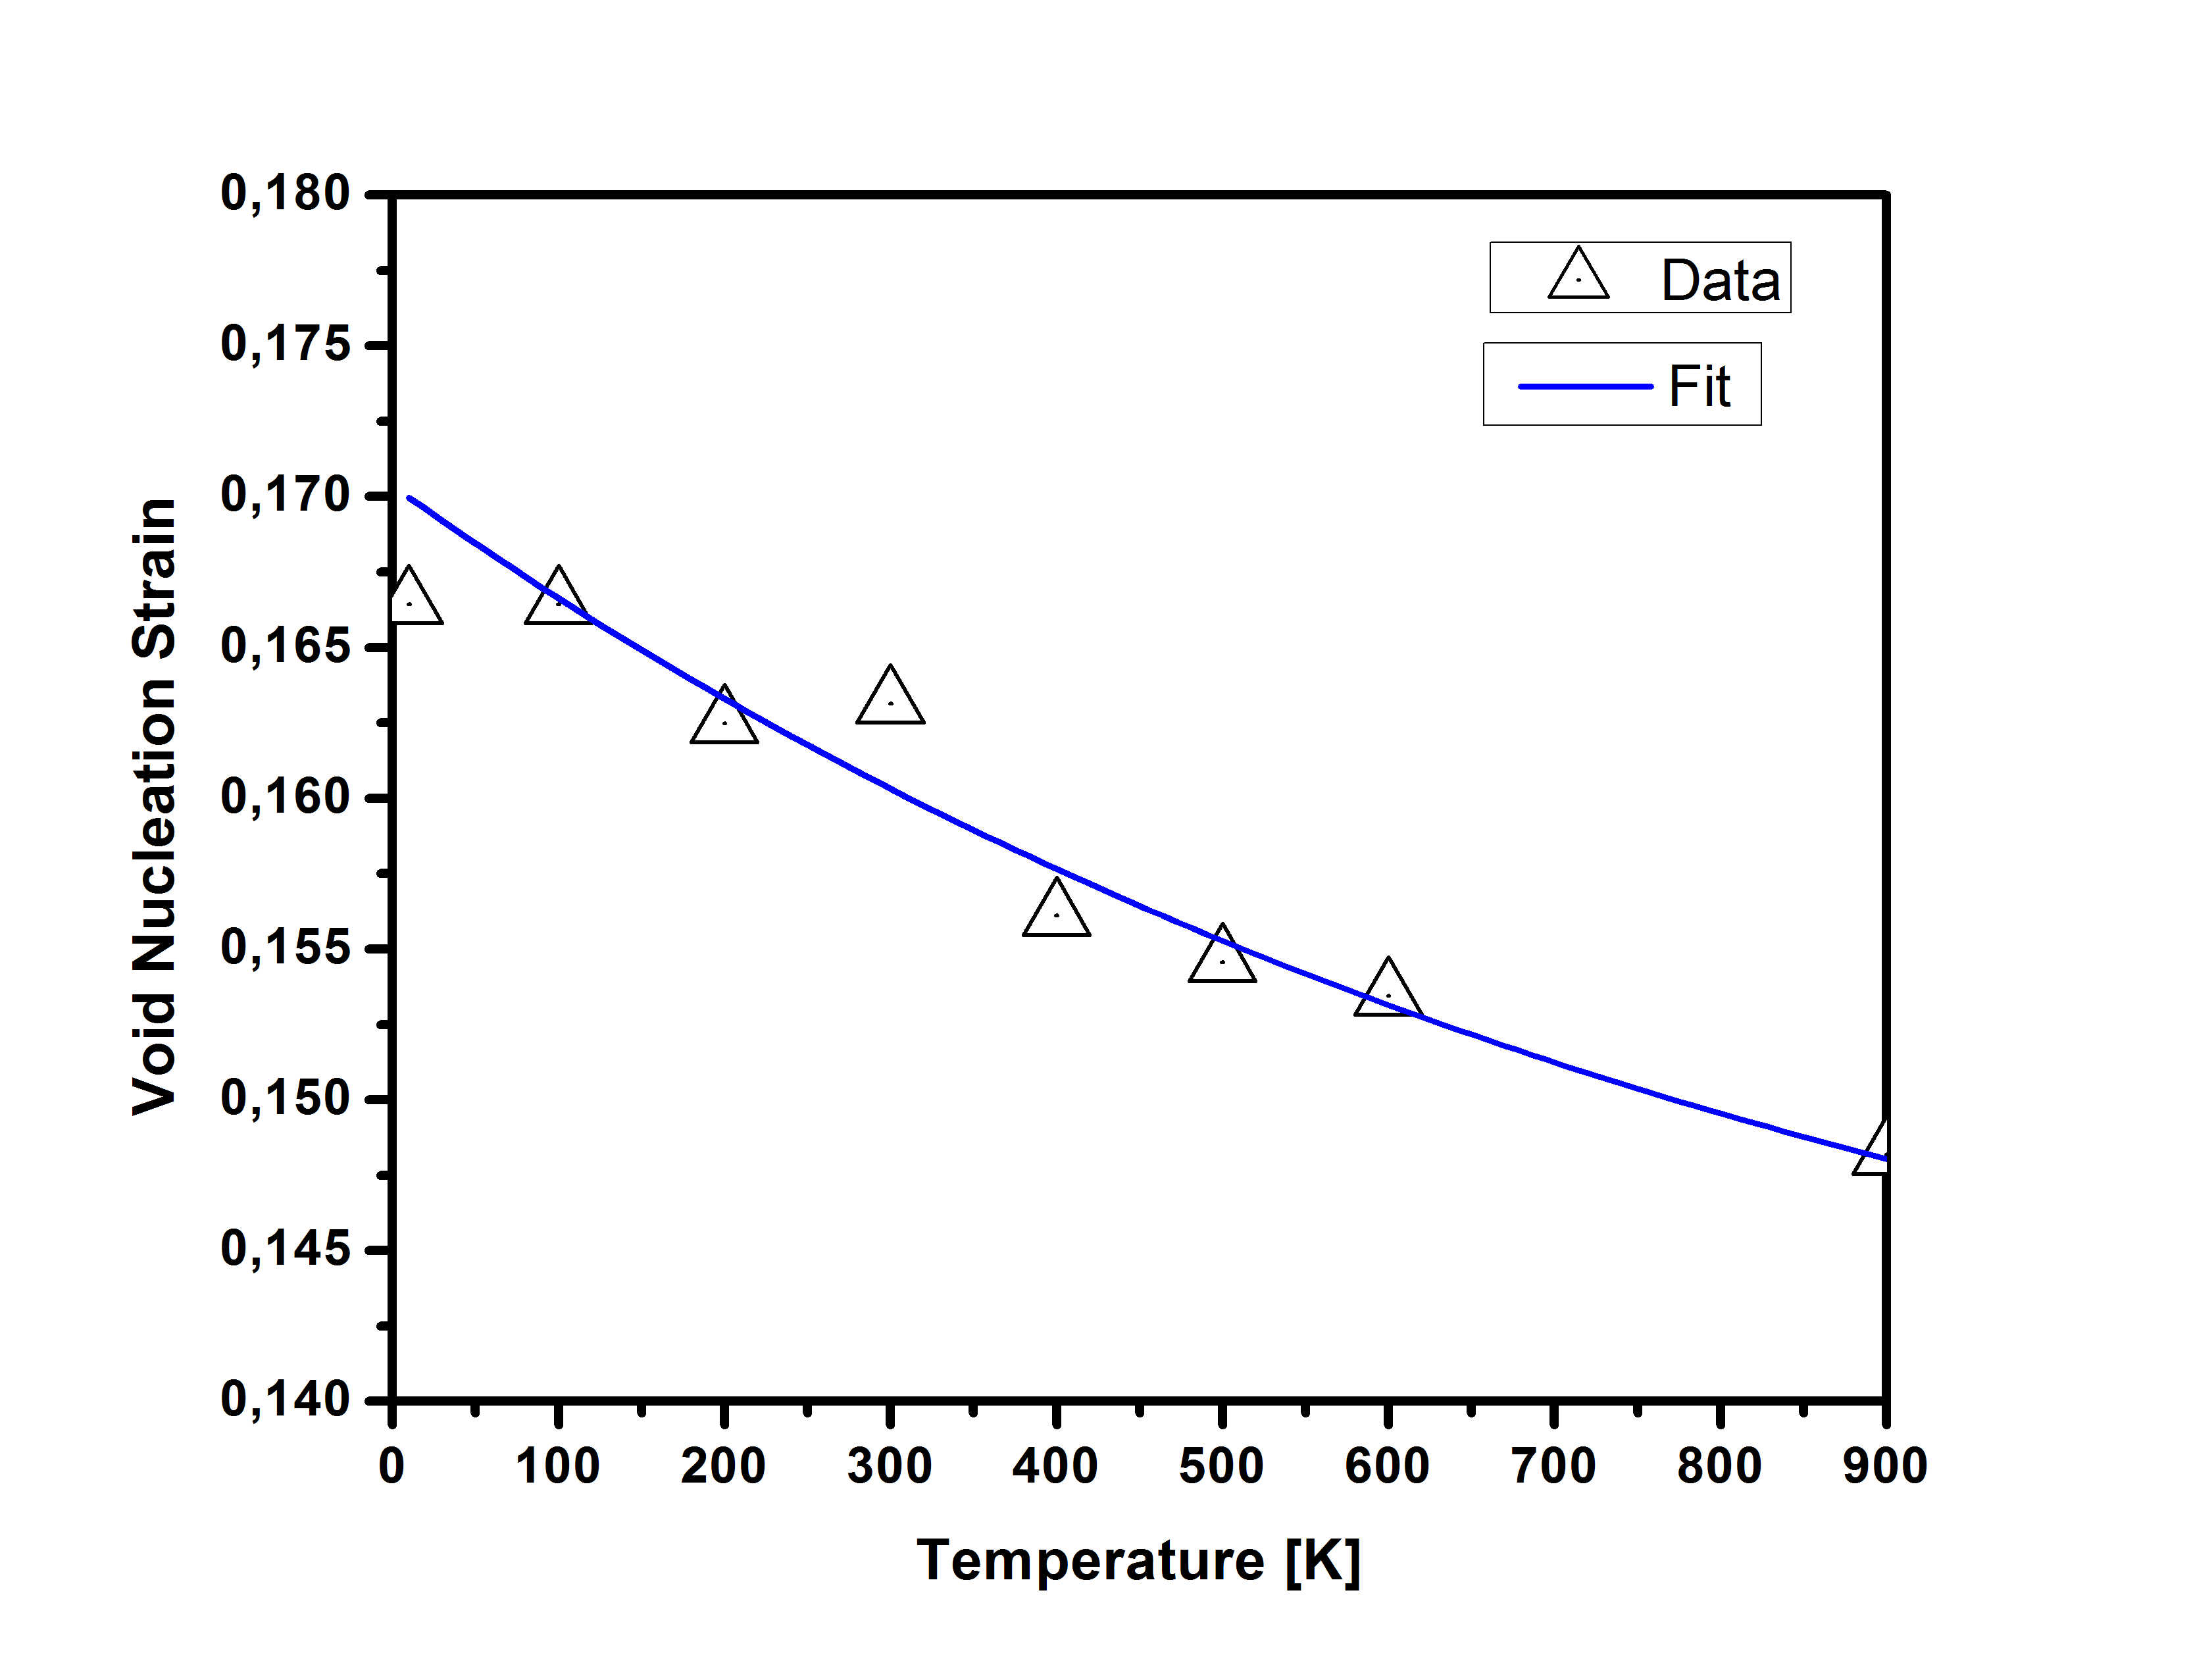
\includegraphics[width=8cm]{Figures/VoidNucleationStrain_Vs_Temp_TENSION.png}
\caption{Strains de nucleacion de void vs. temperatura}
\end{figure}

\begin{figure}[H]
\centering
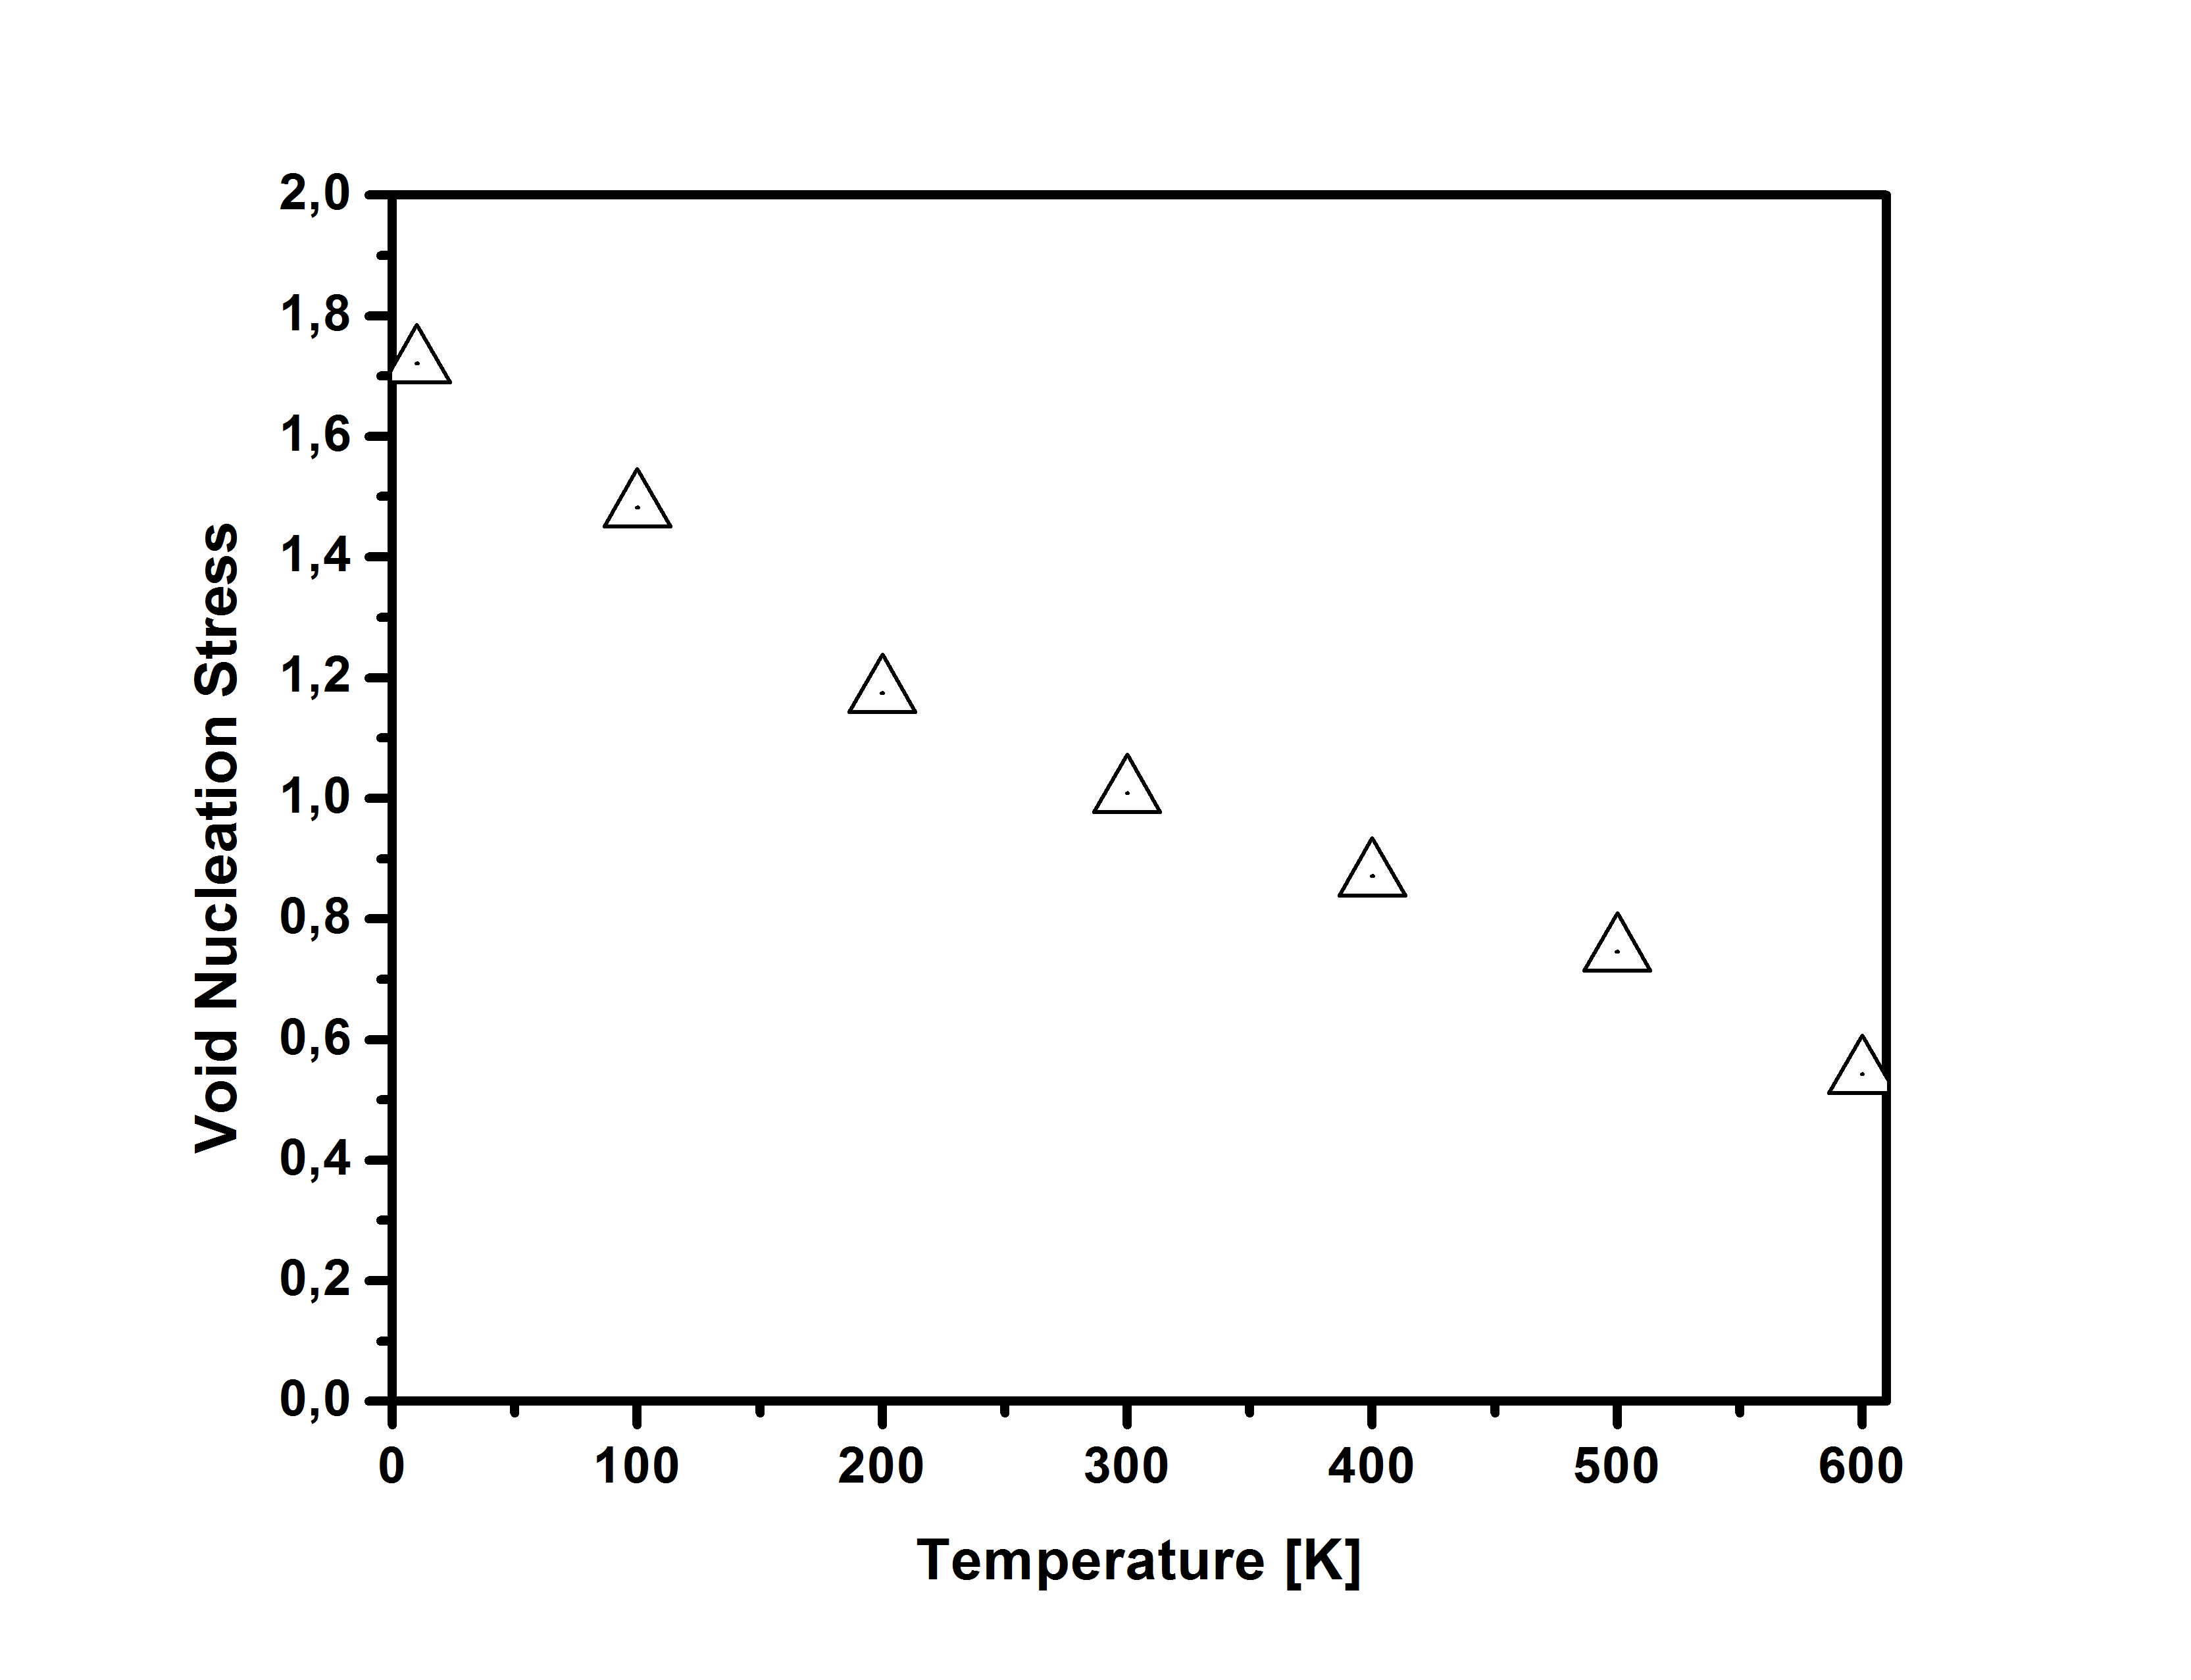
\includegraphics[width=8cm]{Figures/VoidNucleationStress_Vs_Temp_TENSION.png}
\caption{Stress de nucleacion de void vs. temperatura}
\end{figure}

\begin{figure}[H]
\centering
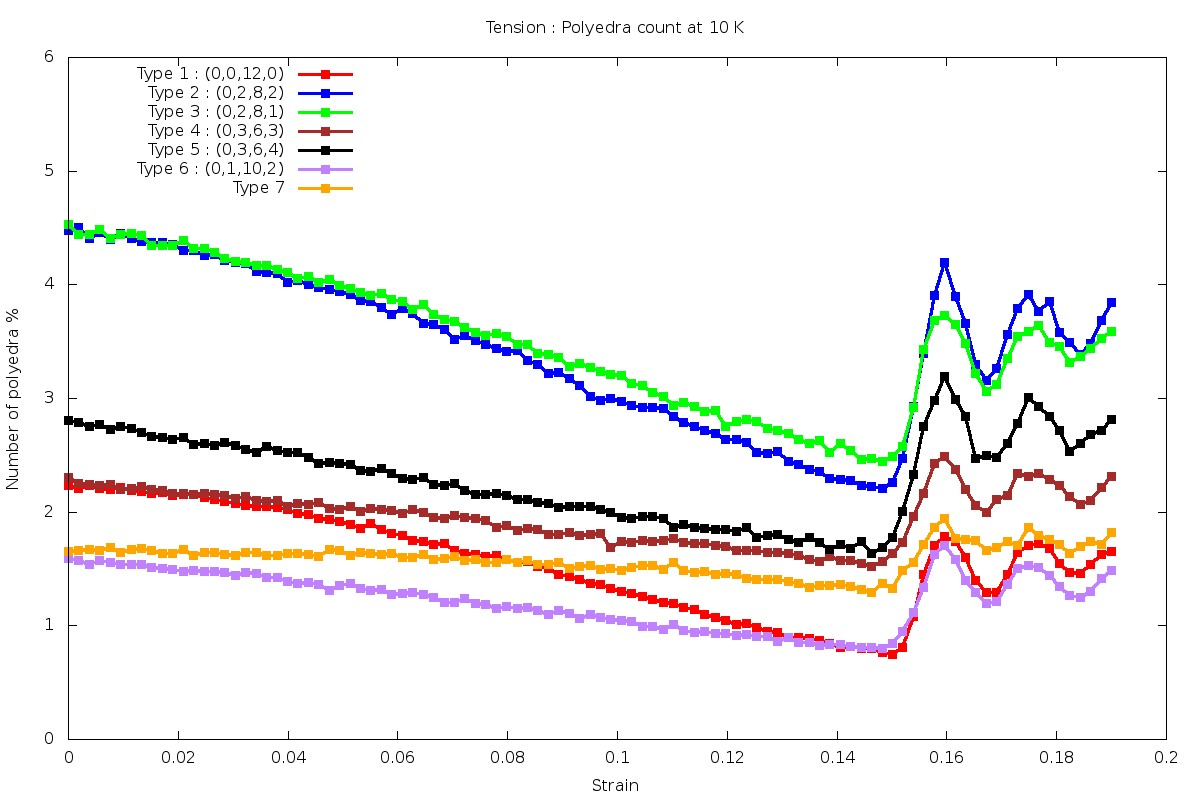
\includegraphics[width=8cm]{Figures/Tens_Polyedra_10K.jpeg}
\caption{Polyedros de voronoi vs. strain para 10K}
\end{figure}

\begin{figure}[H]
\centering
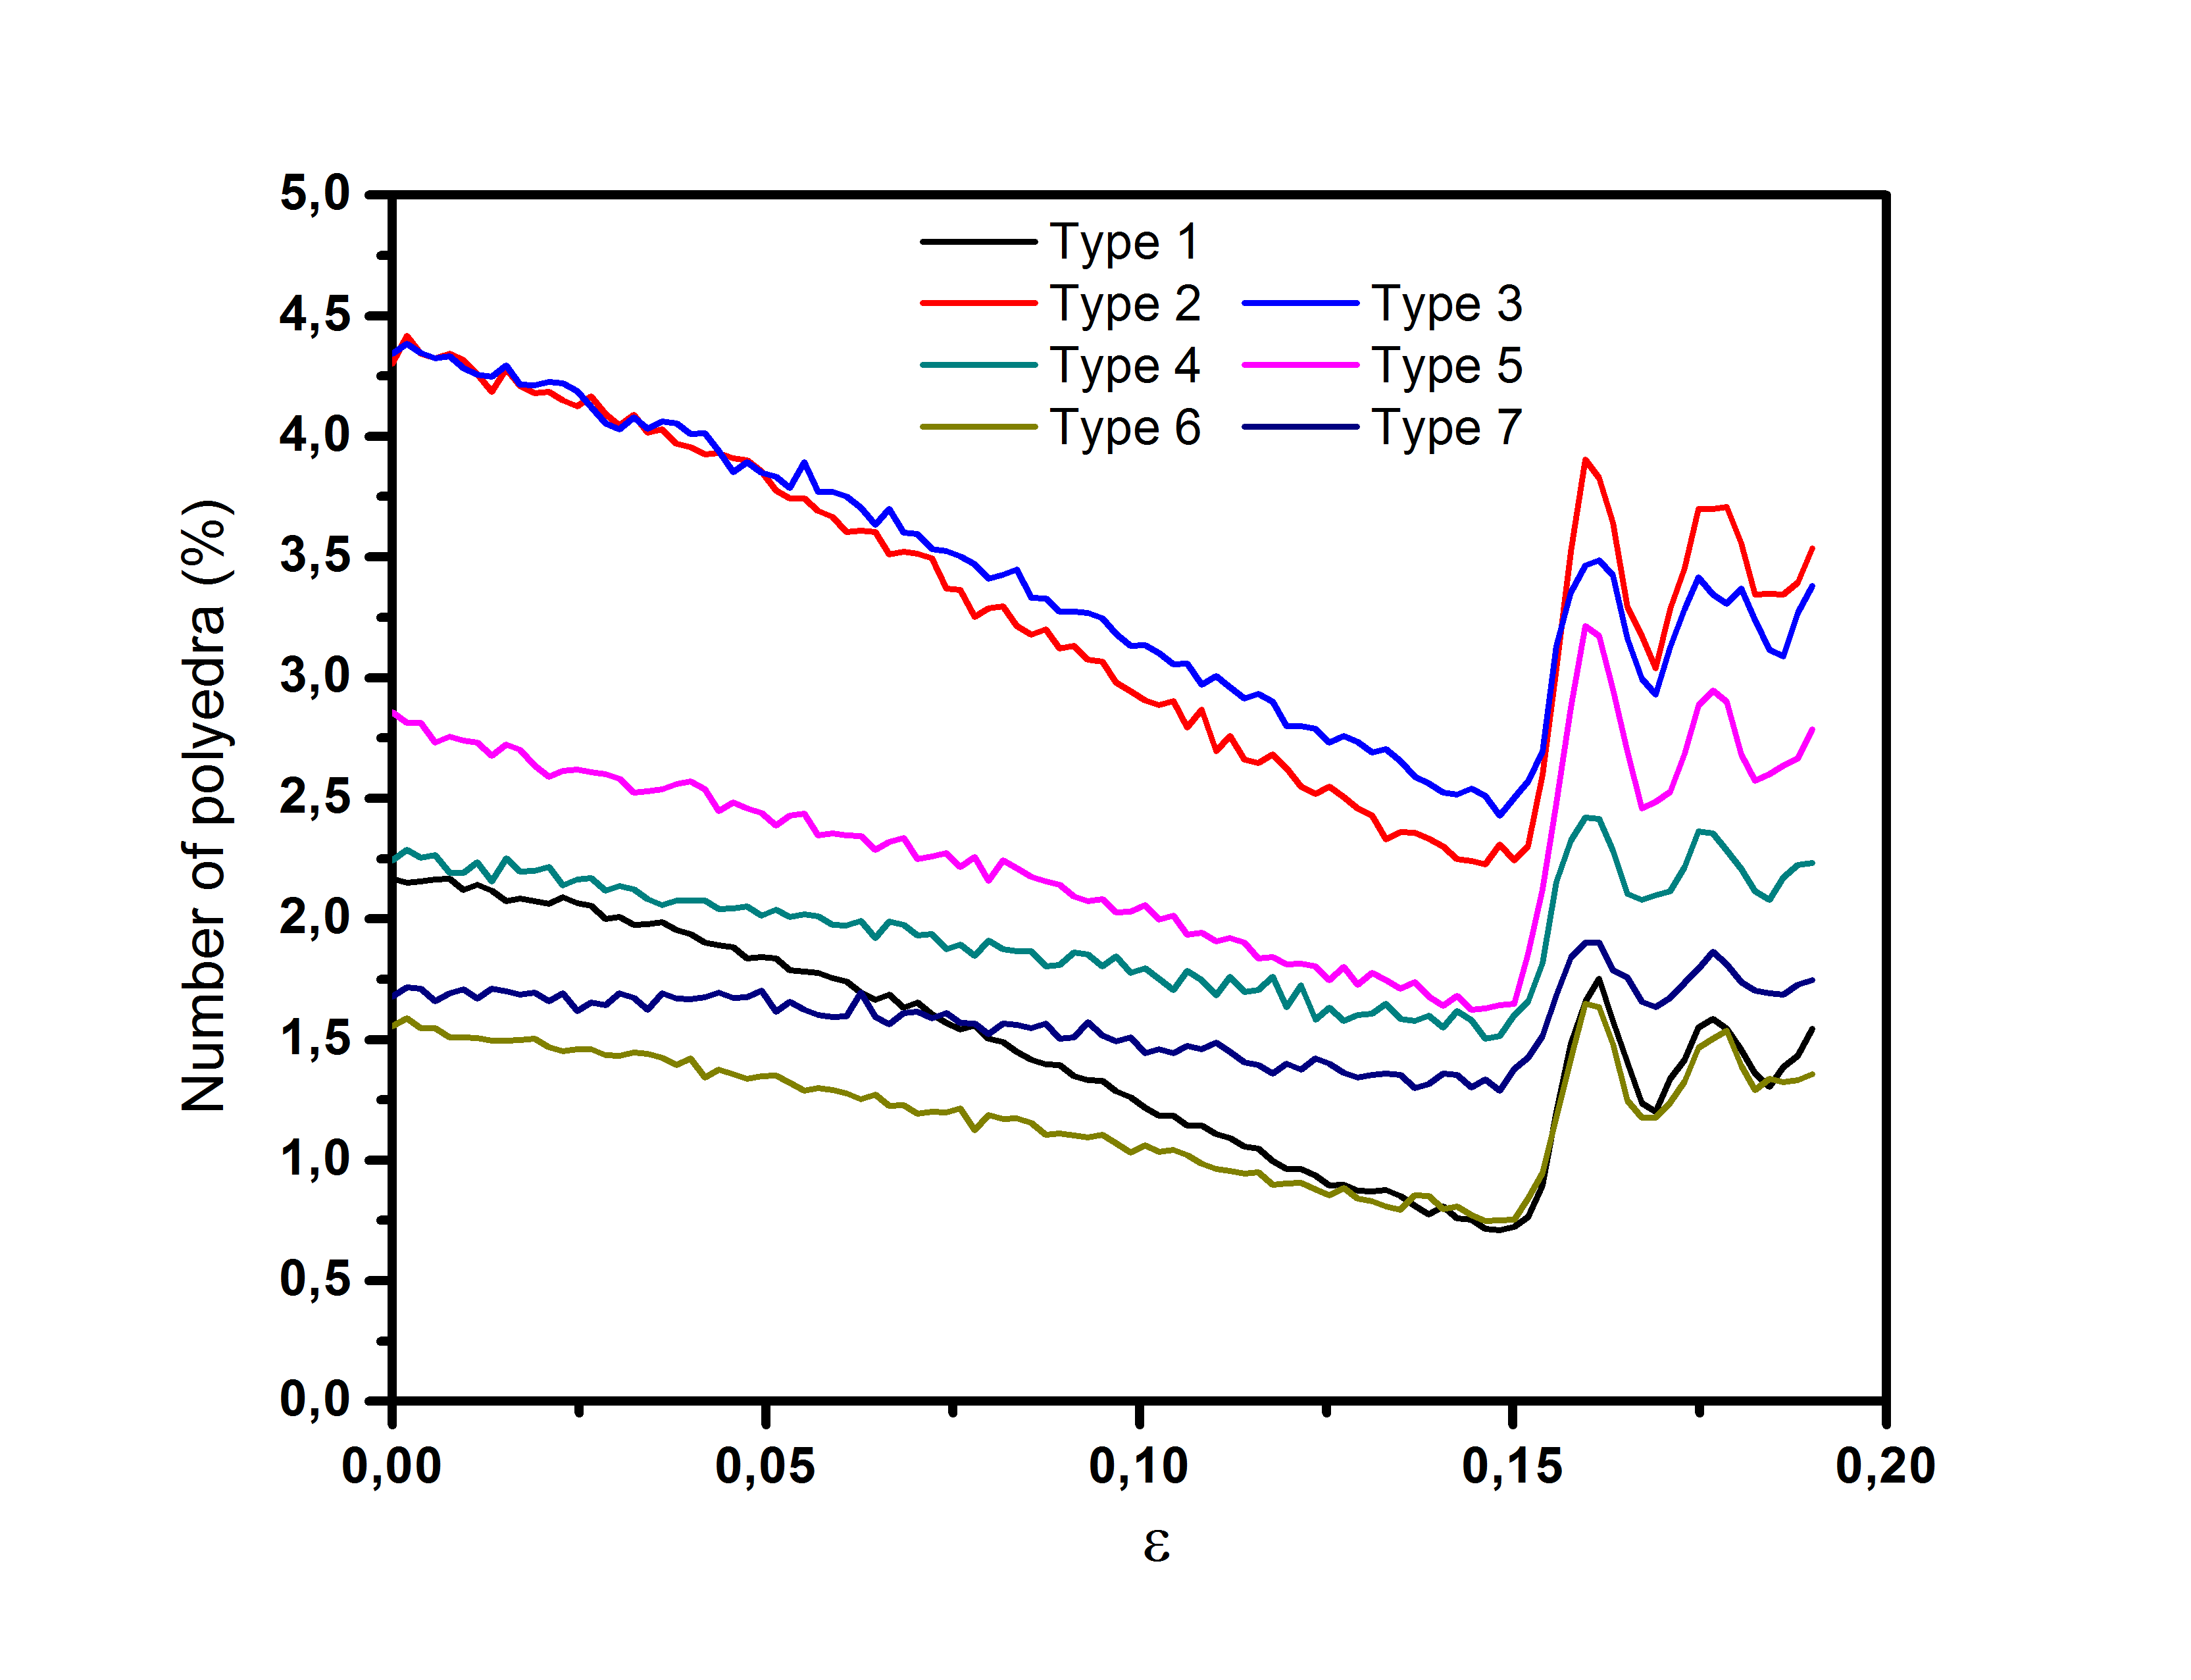
\includegraphics[width=8cm]{Figures/Polyedra_Vs_Strain_100K_TEN.png}
\caption{Num polyedros de voronoi vs. strain, a 100K}
\end{figure}

\begin{figure}[H]
\centering
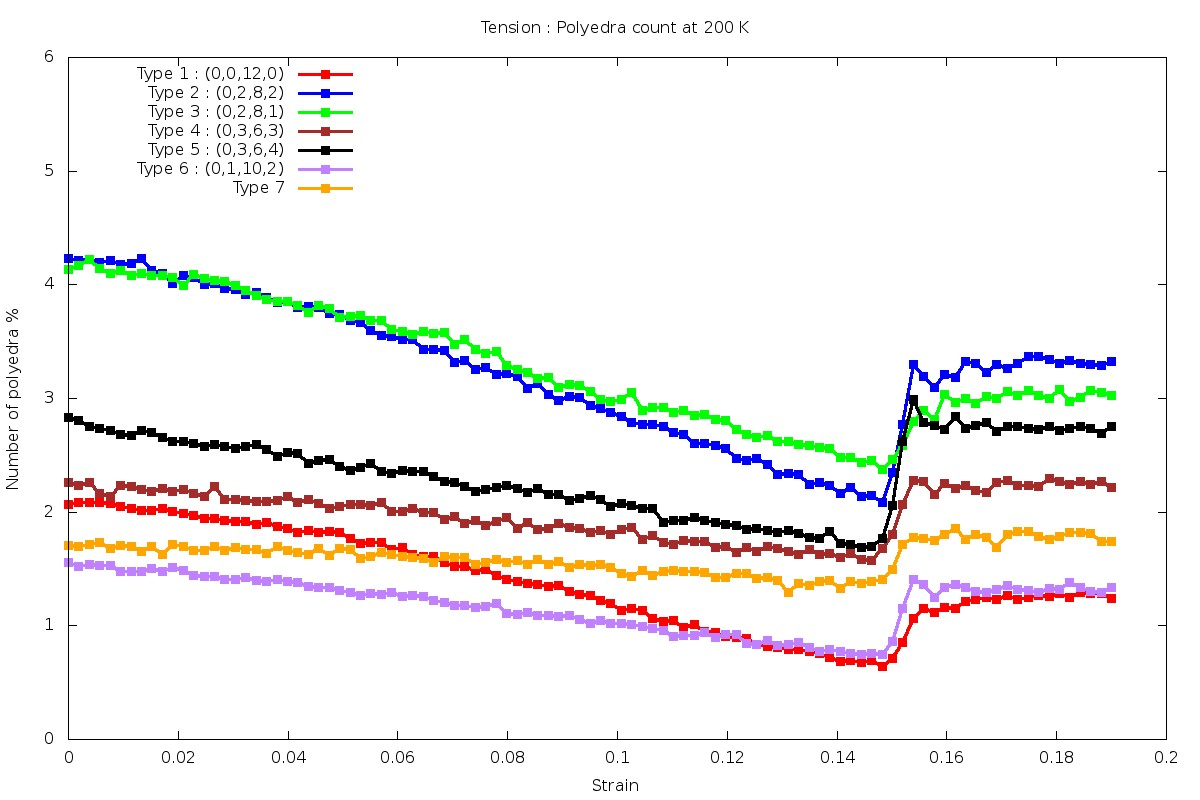
\includegraphics[width=8cm]{Figures/Tens_Polyedra_200K.jpeg}
\caption{Polyedros de voronoi vs. strain para 200K}
\end{figure}

\begin{figure}[H]
\centering
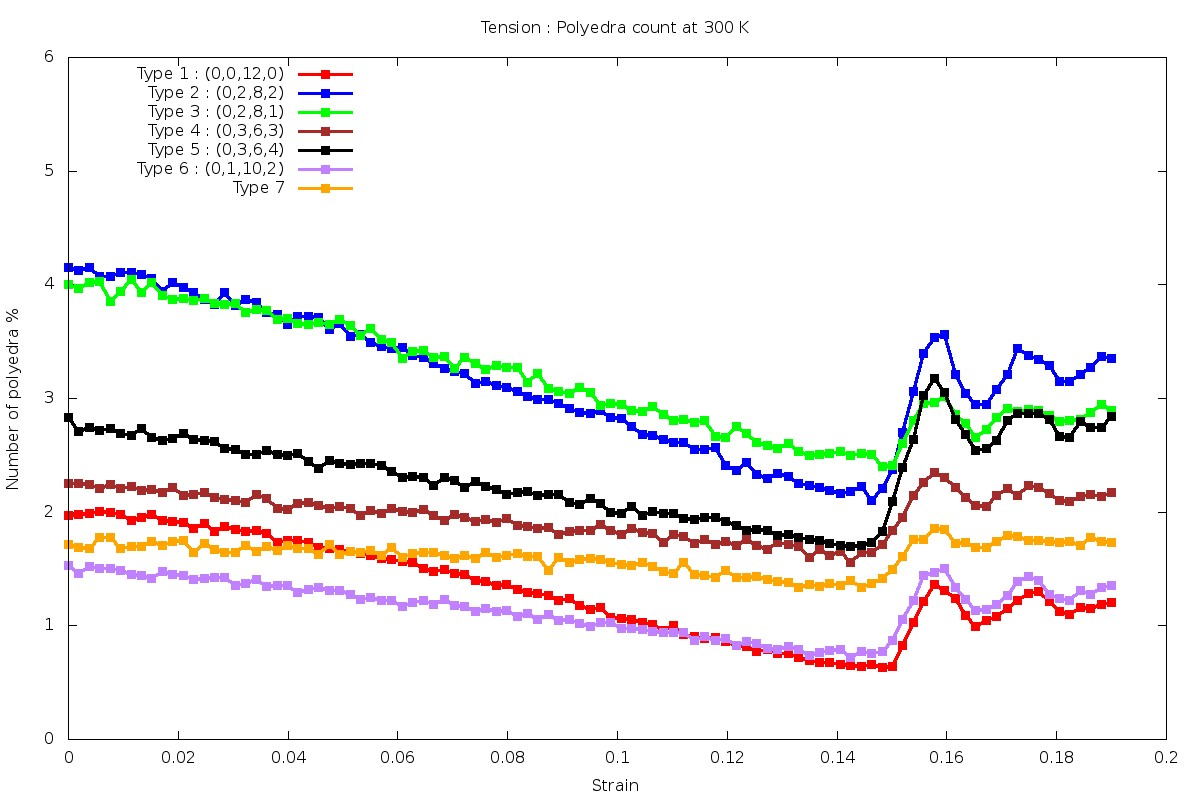
\includegraphics[width=8cm]{Figures/Tens_Polyedra_300K.jpeg}
\caption{Polyedros de voronoi vs. strain para 300K}
\end{figure}

\begin{figure}[H]
\centering
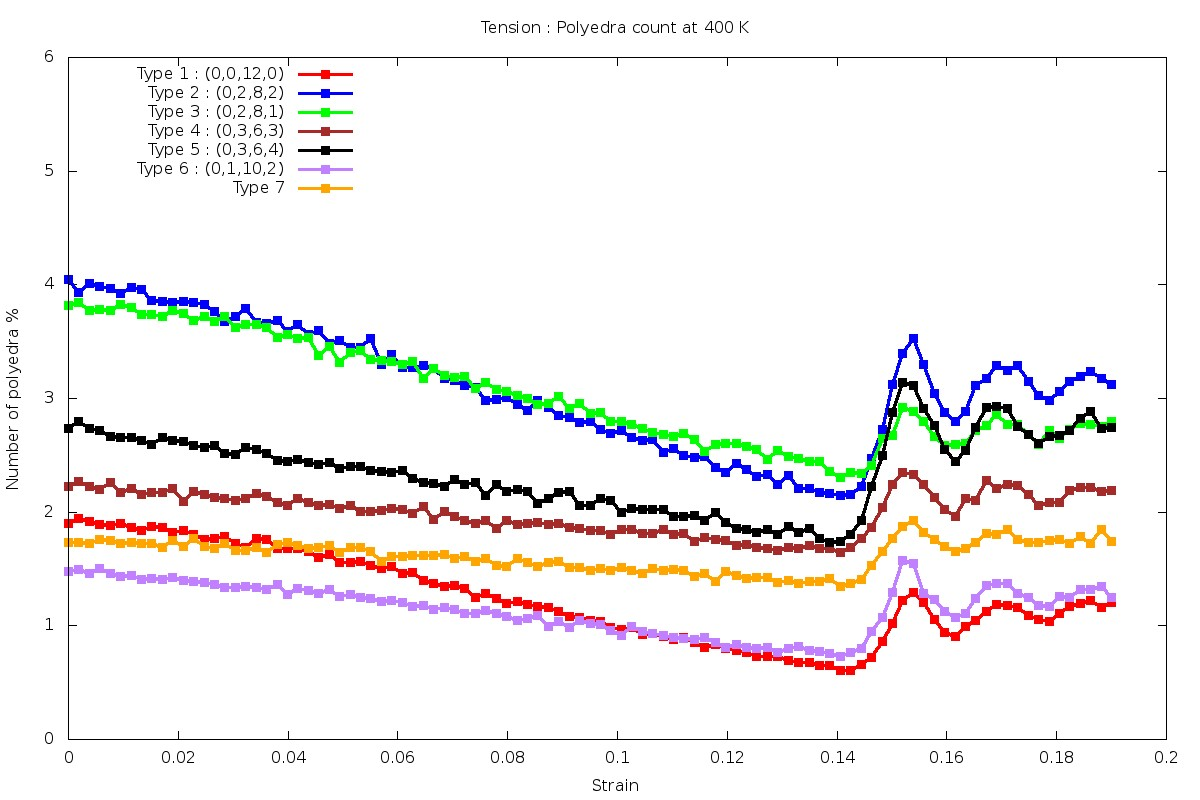
\includegraphics[width=8cm]{Figures/Tens_Polyedra_400K.jpeg}
\caption{Polyedros de voronoi vs. strain para 400K}
\end{figure}

\begin{figure}[H]
\centering
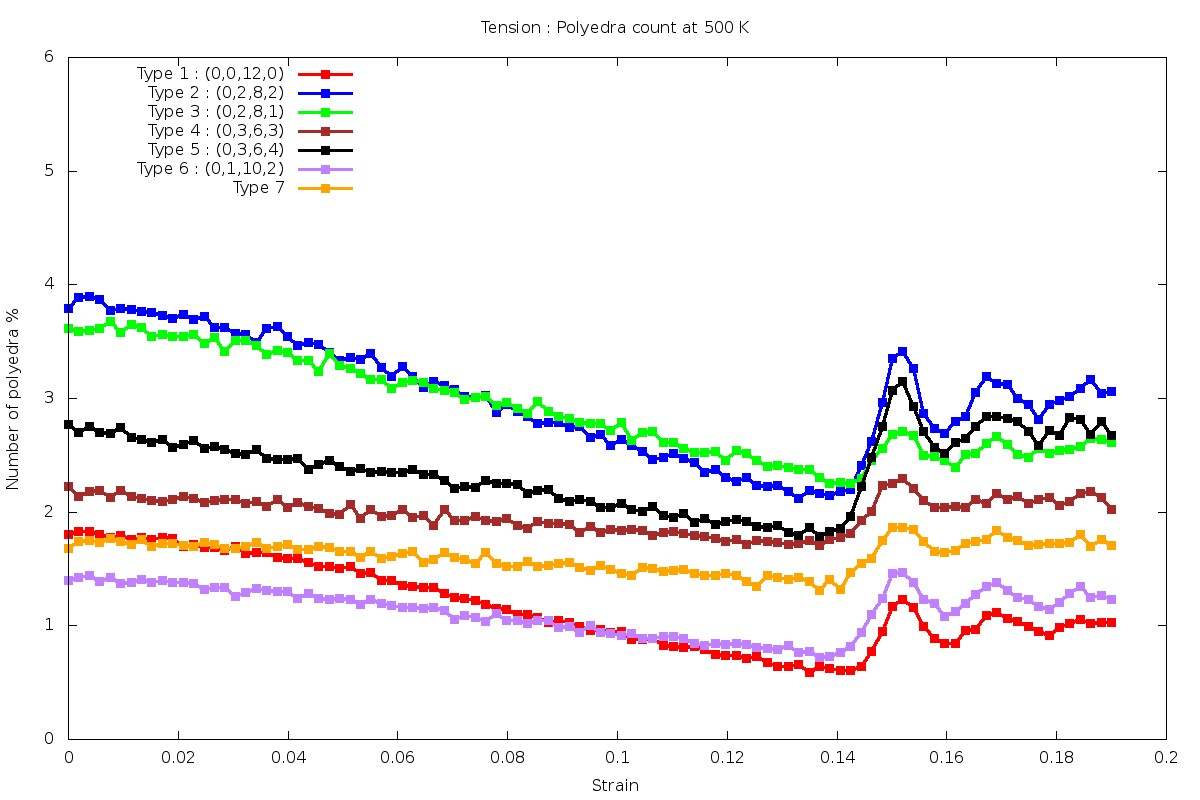
\includegraphics[width=8cm]{Figures/Tens_Polyedra_500K.jpeg}
\caption{Polyedros de voronoi vs. strain para 500K}
\end{figure}

\begin{figure}[H]
\centering
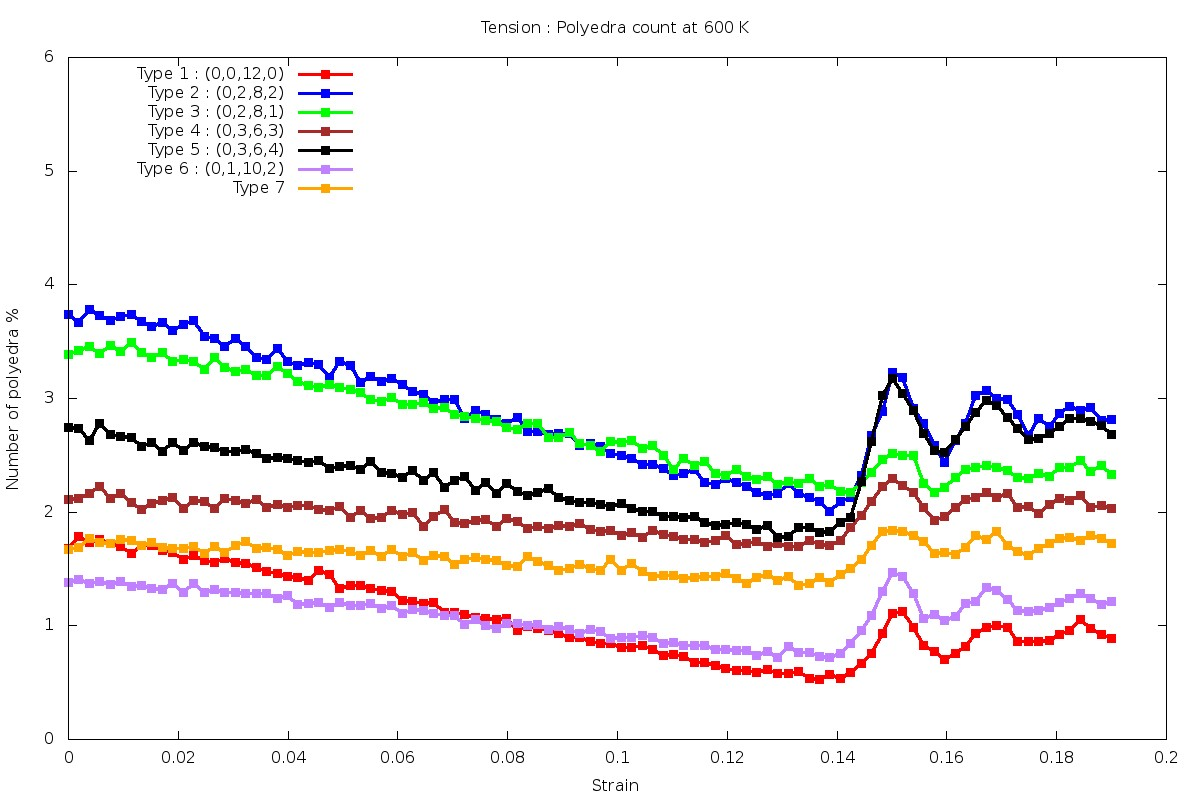
\includegraphics[width=8cm]{Figures/Tens_Polyedra_600K.jpeg}
\caption{Polyedros de voronoi vs. strain para 600K}
\end{figure}

\begin{figure}[H]
\centering
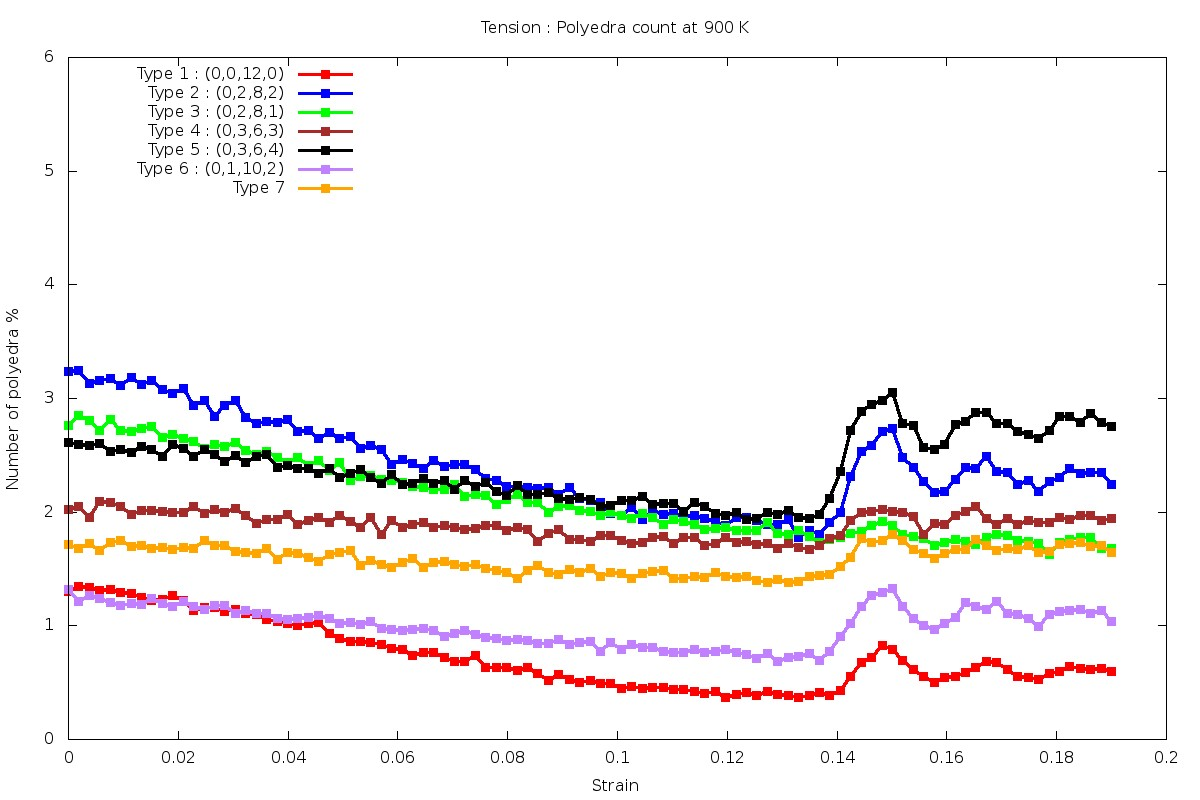
\includegraphics[width=8cm]{Figures/Tens_Polyedra_900K.jpeg}
\caption{Polyedros de voronoi vs. strain para 900K}
\end{figure}

\begin{figure}[H]
\centering
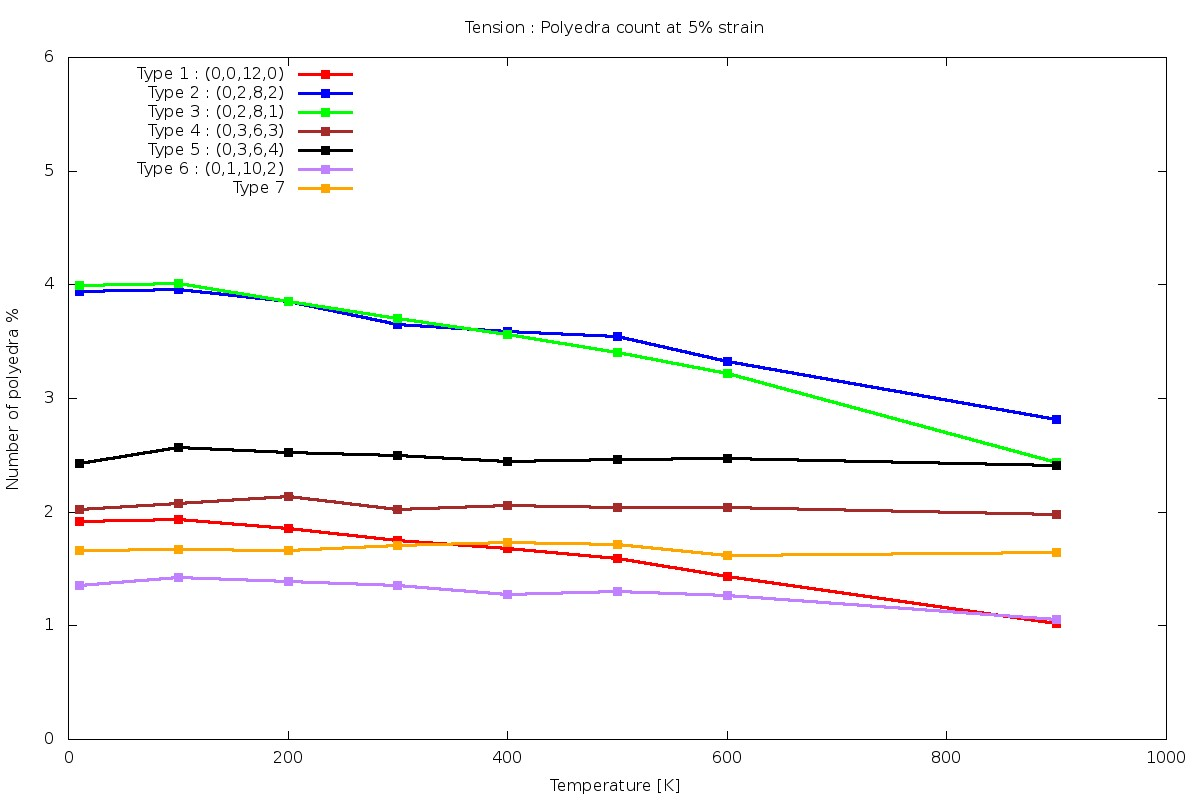
\includegraphics[width=8cm]{Figures/Tension_Voro_Temp_5.jpeg}
\caption{Num polyedros de voronoi vs. temperatura, a strain 5\%}
\end{figure}

\begin{figure}[H]
\centering
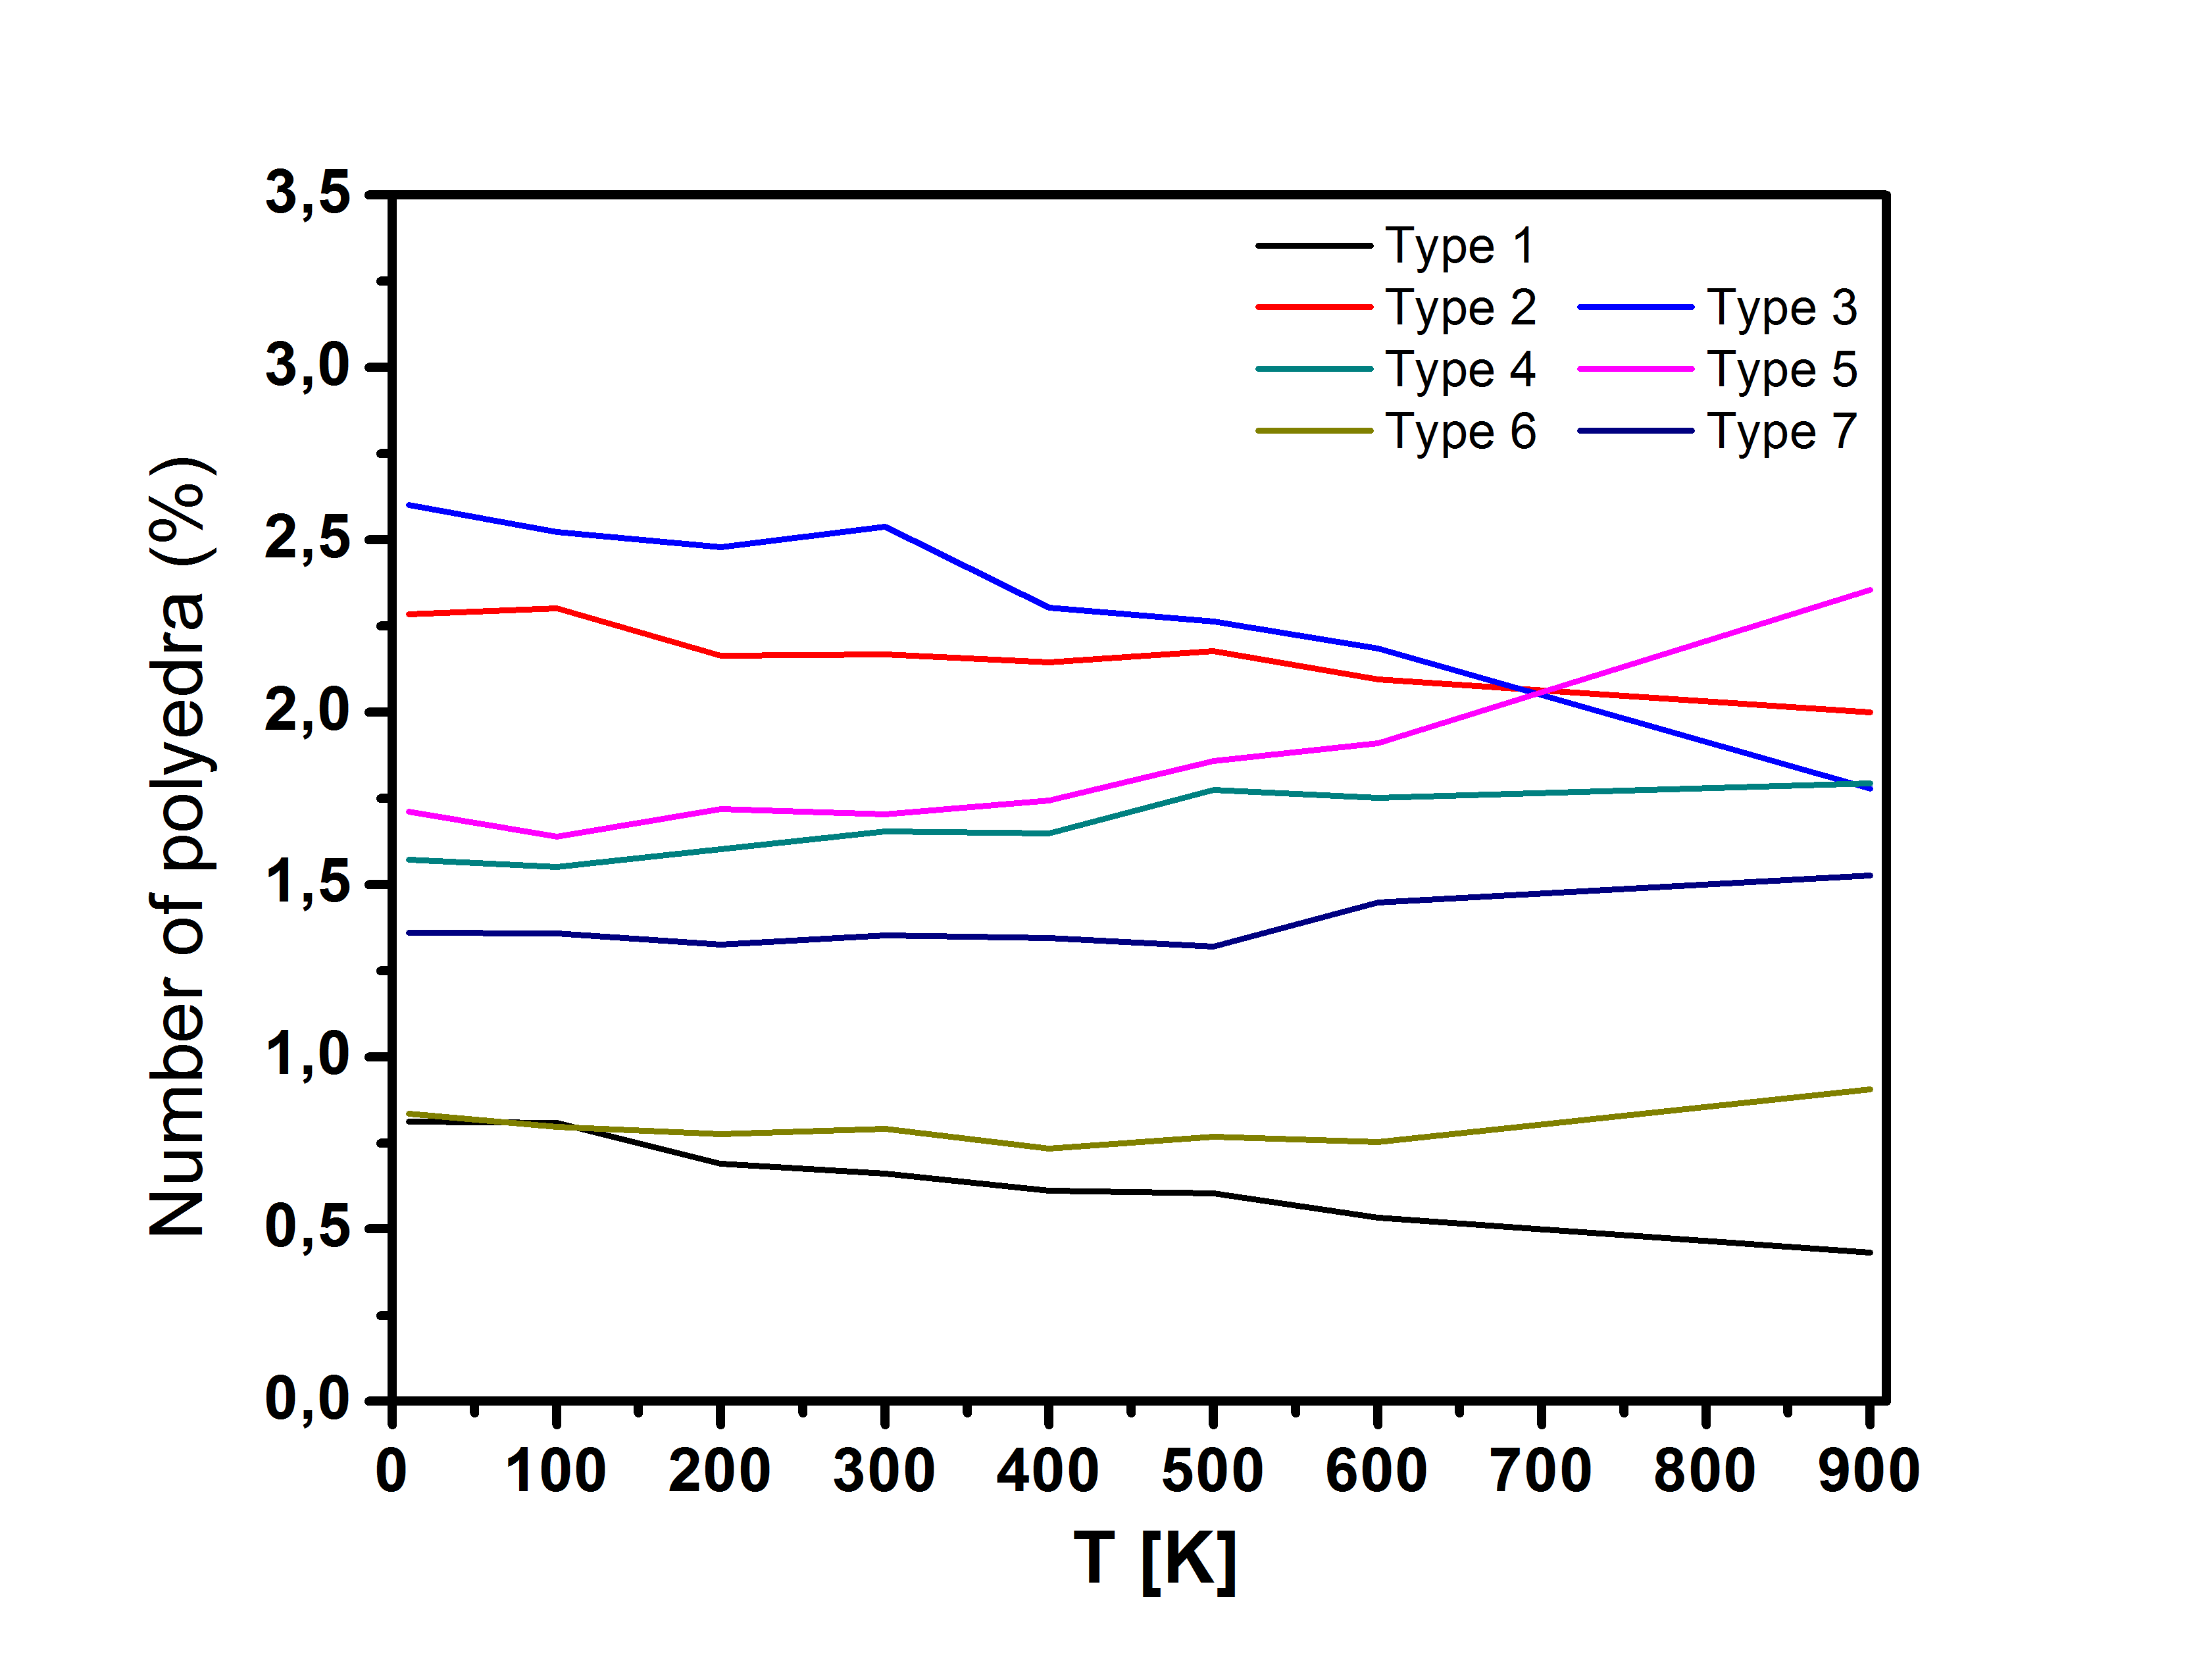
\includegraphics[width=8cm]{Figures/poly_T_14strain_TEN.png}
\caption{Num polyedros de voronoi vs. temperatura, a strain 14\%}
\end{figure}

\begin{figure}[H]
\centering
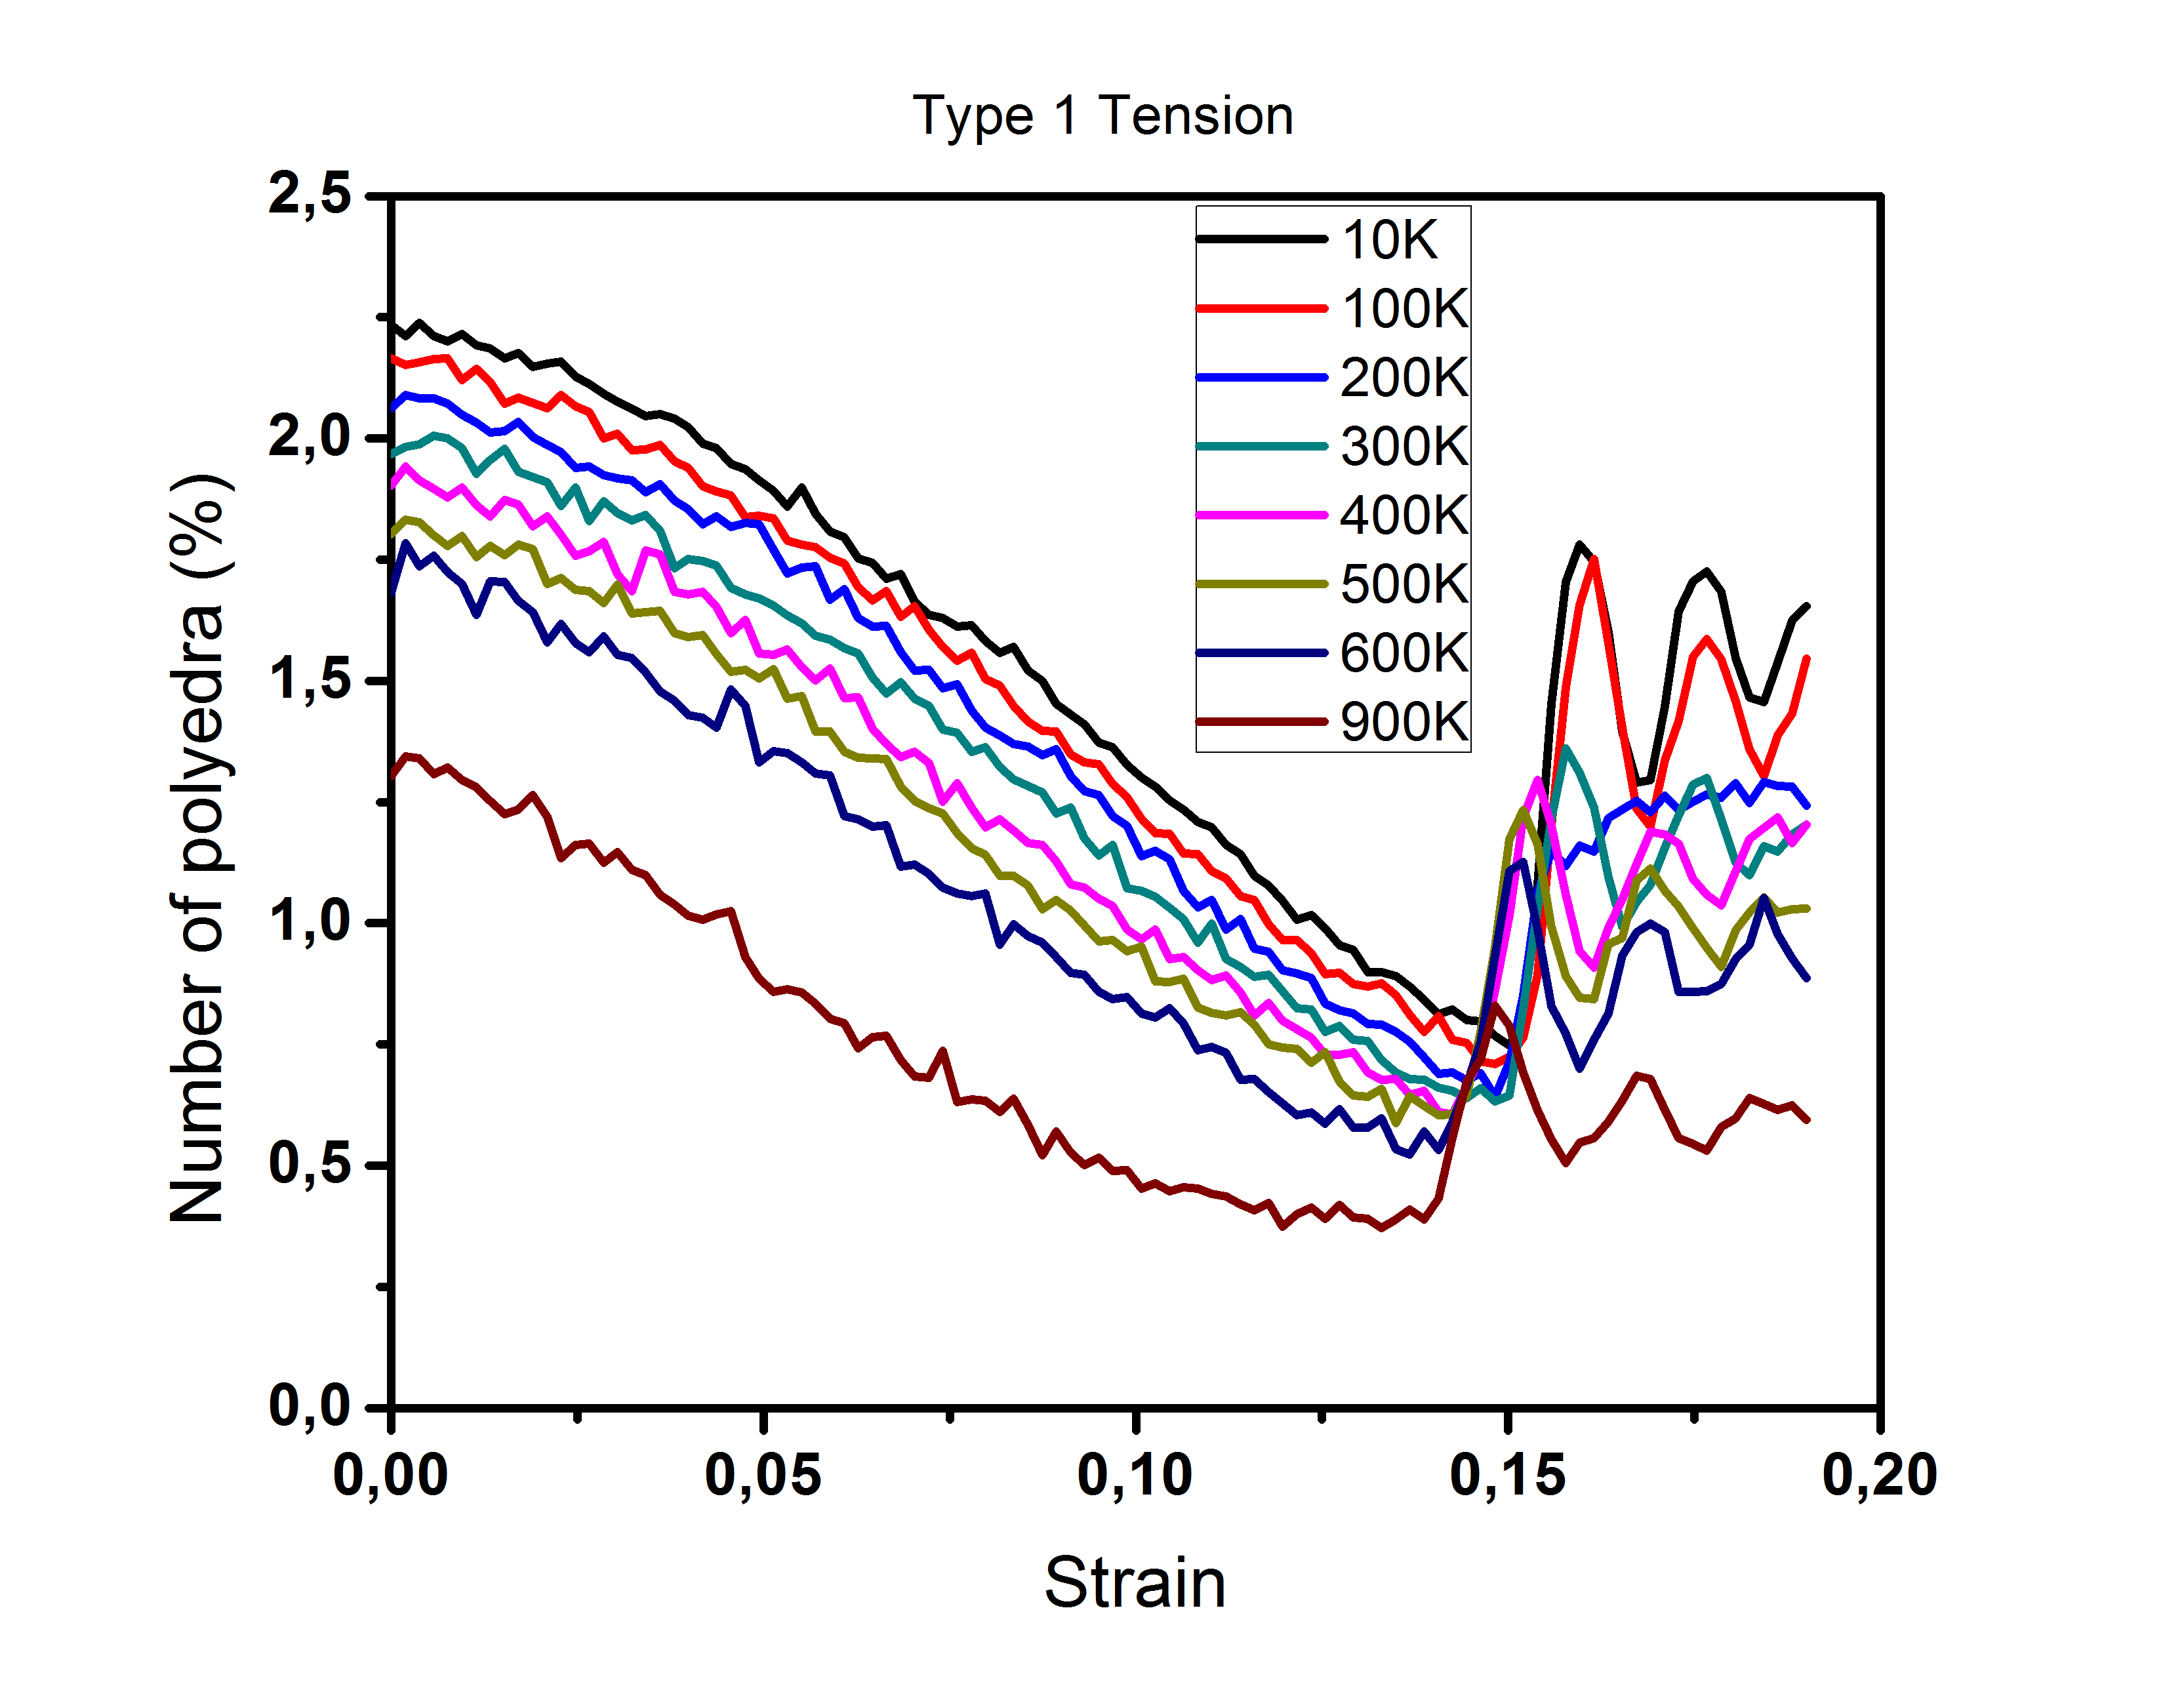
\includegraphics[width=8cm]{Figures/type1_TEN.png}
\caption{polyedros de voronoi tipo 1 vs. strain}
\end{figure}

\begin{figure}[H]
\centering
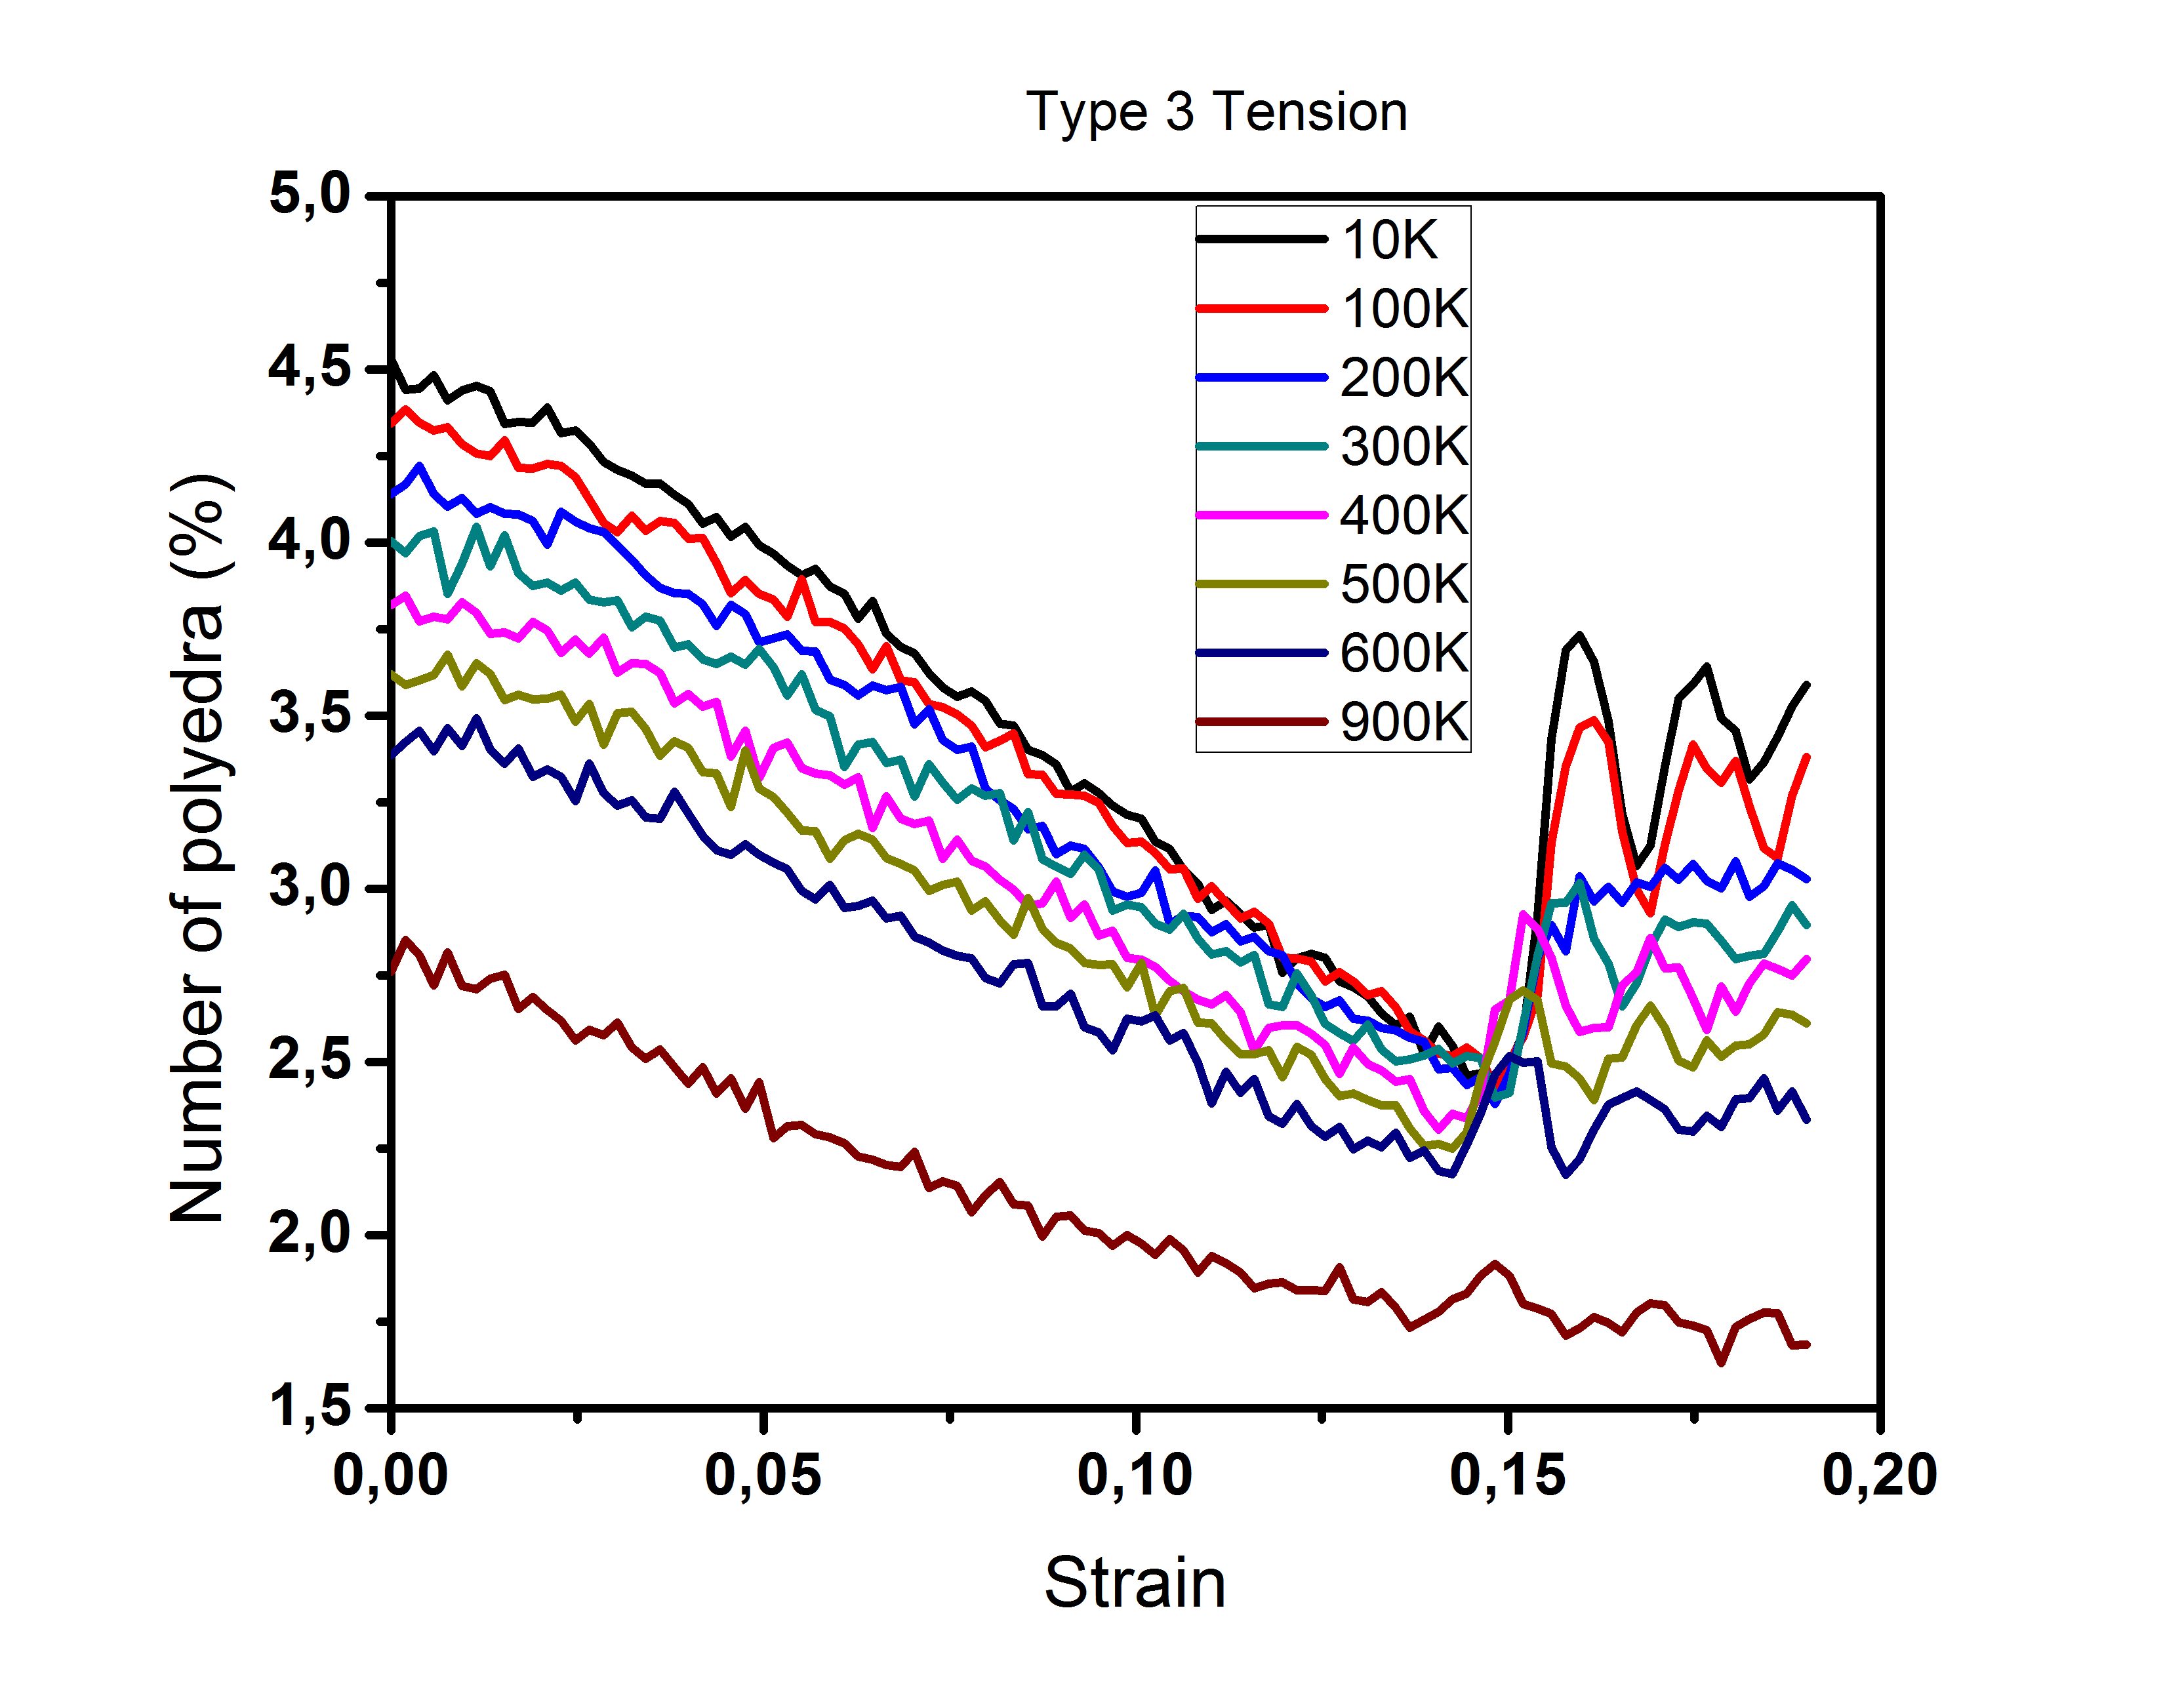
\includegraphics[width=8cm]{Figures/type3_TEN.png}
\caption{polyedros de voronoi tipo 3 vs. strain}
\end{figure}

\begin{figure}[H]
\centering
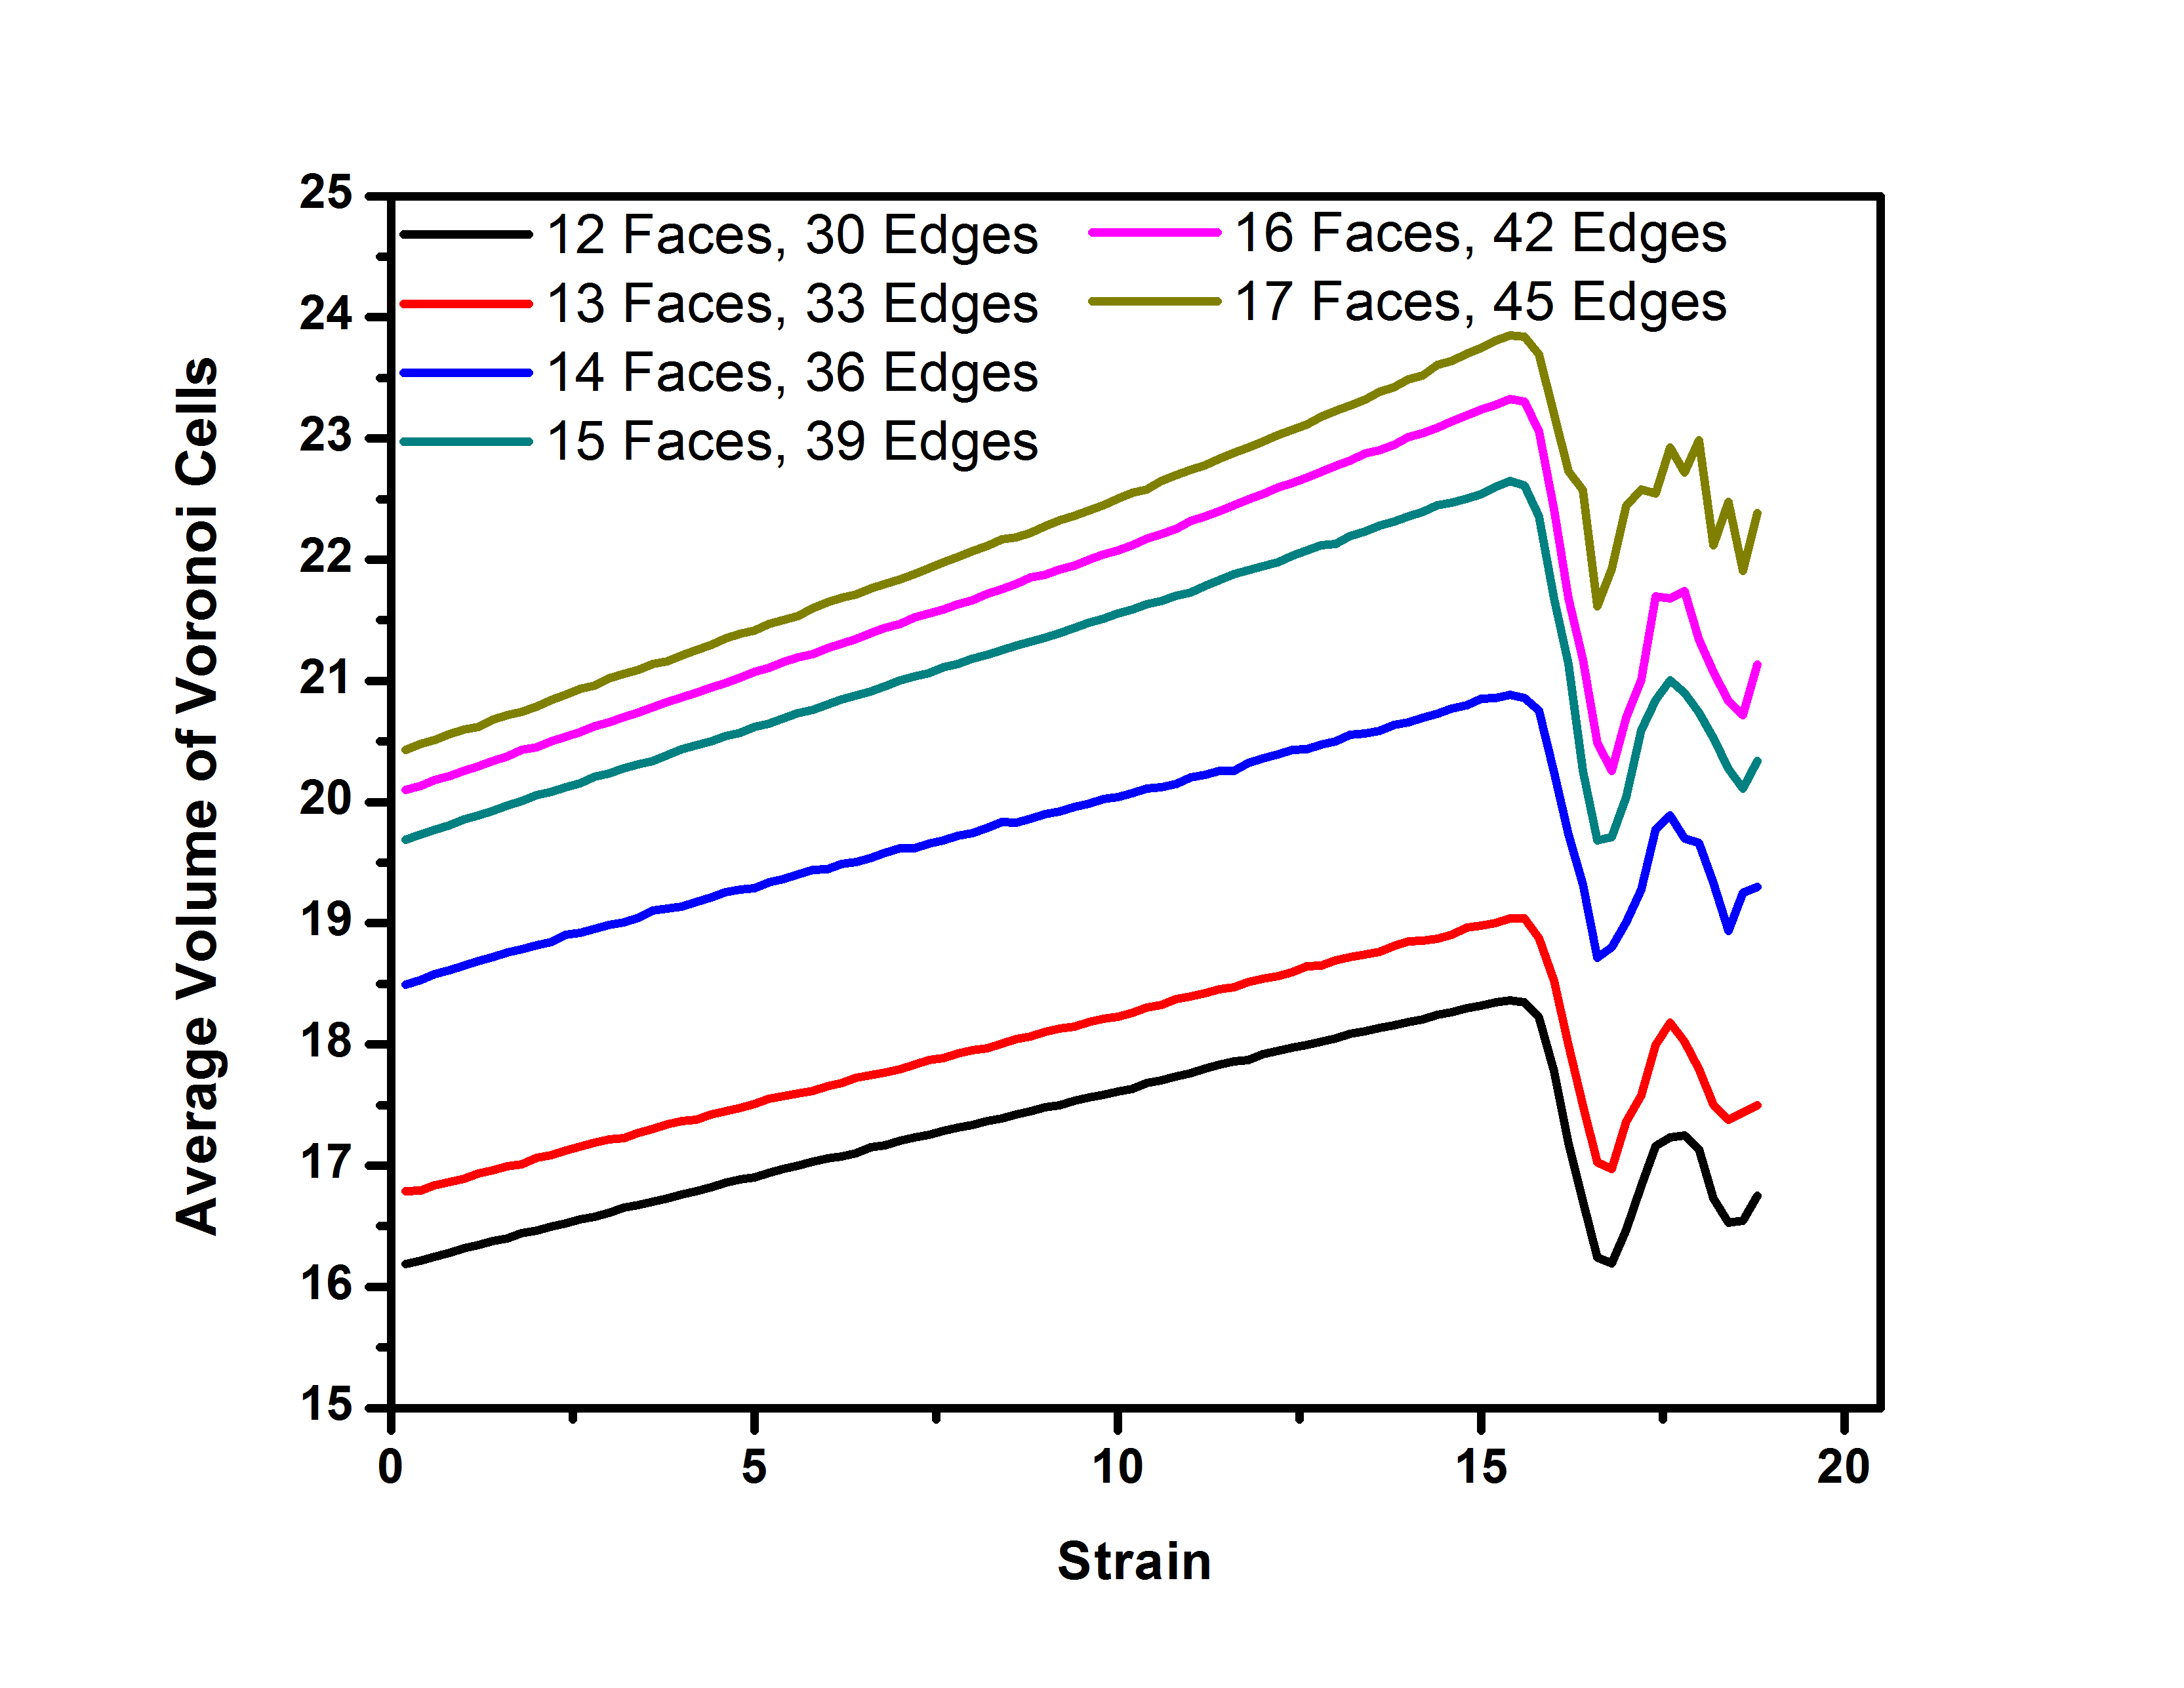
\includegraphics[width=8cm]{Figures/TRAC_Vol_Step_A.png}
\caption{volumen promedio de voronoi cells (parte 1/2, temperatura desconocida)}
\end{figure}

\begin{figure}[H]
\centering
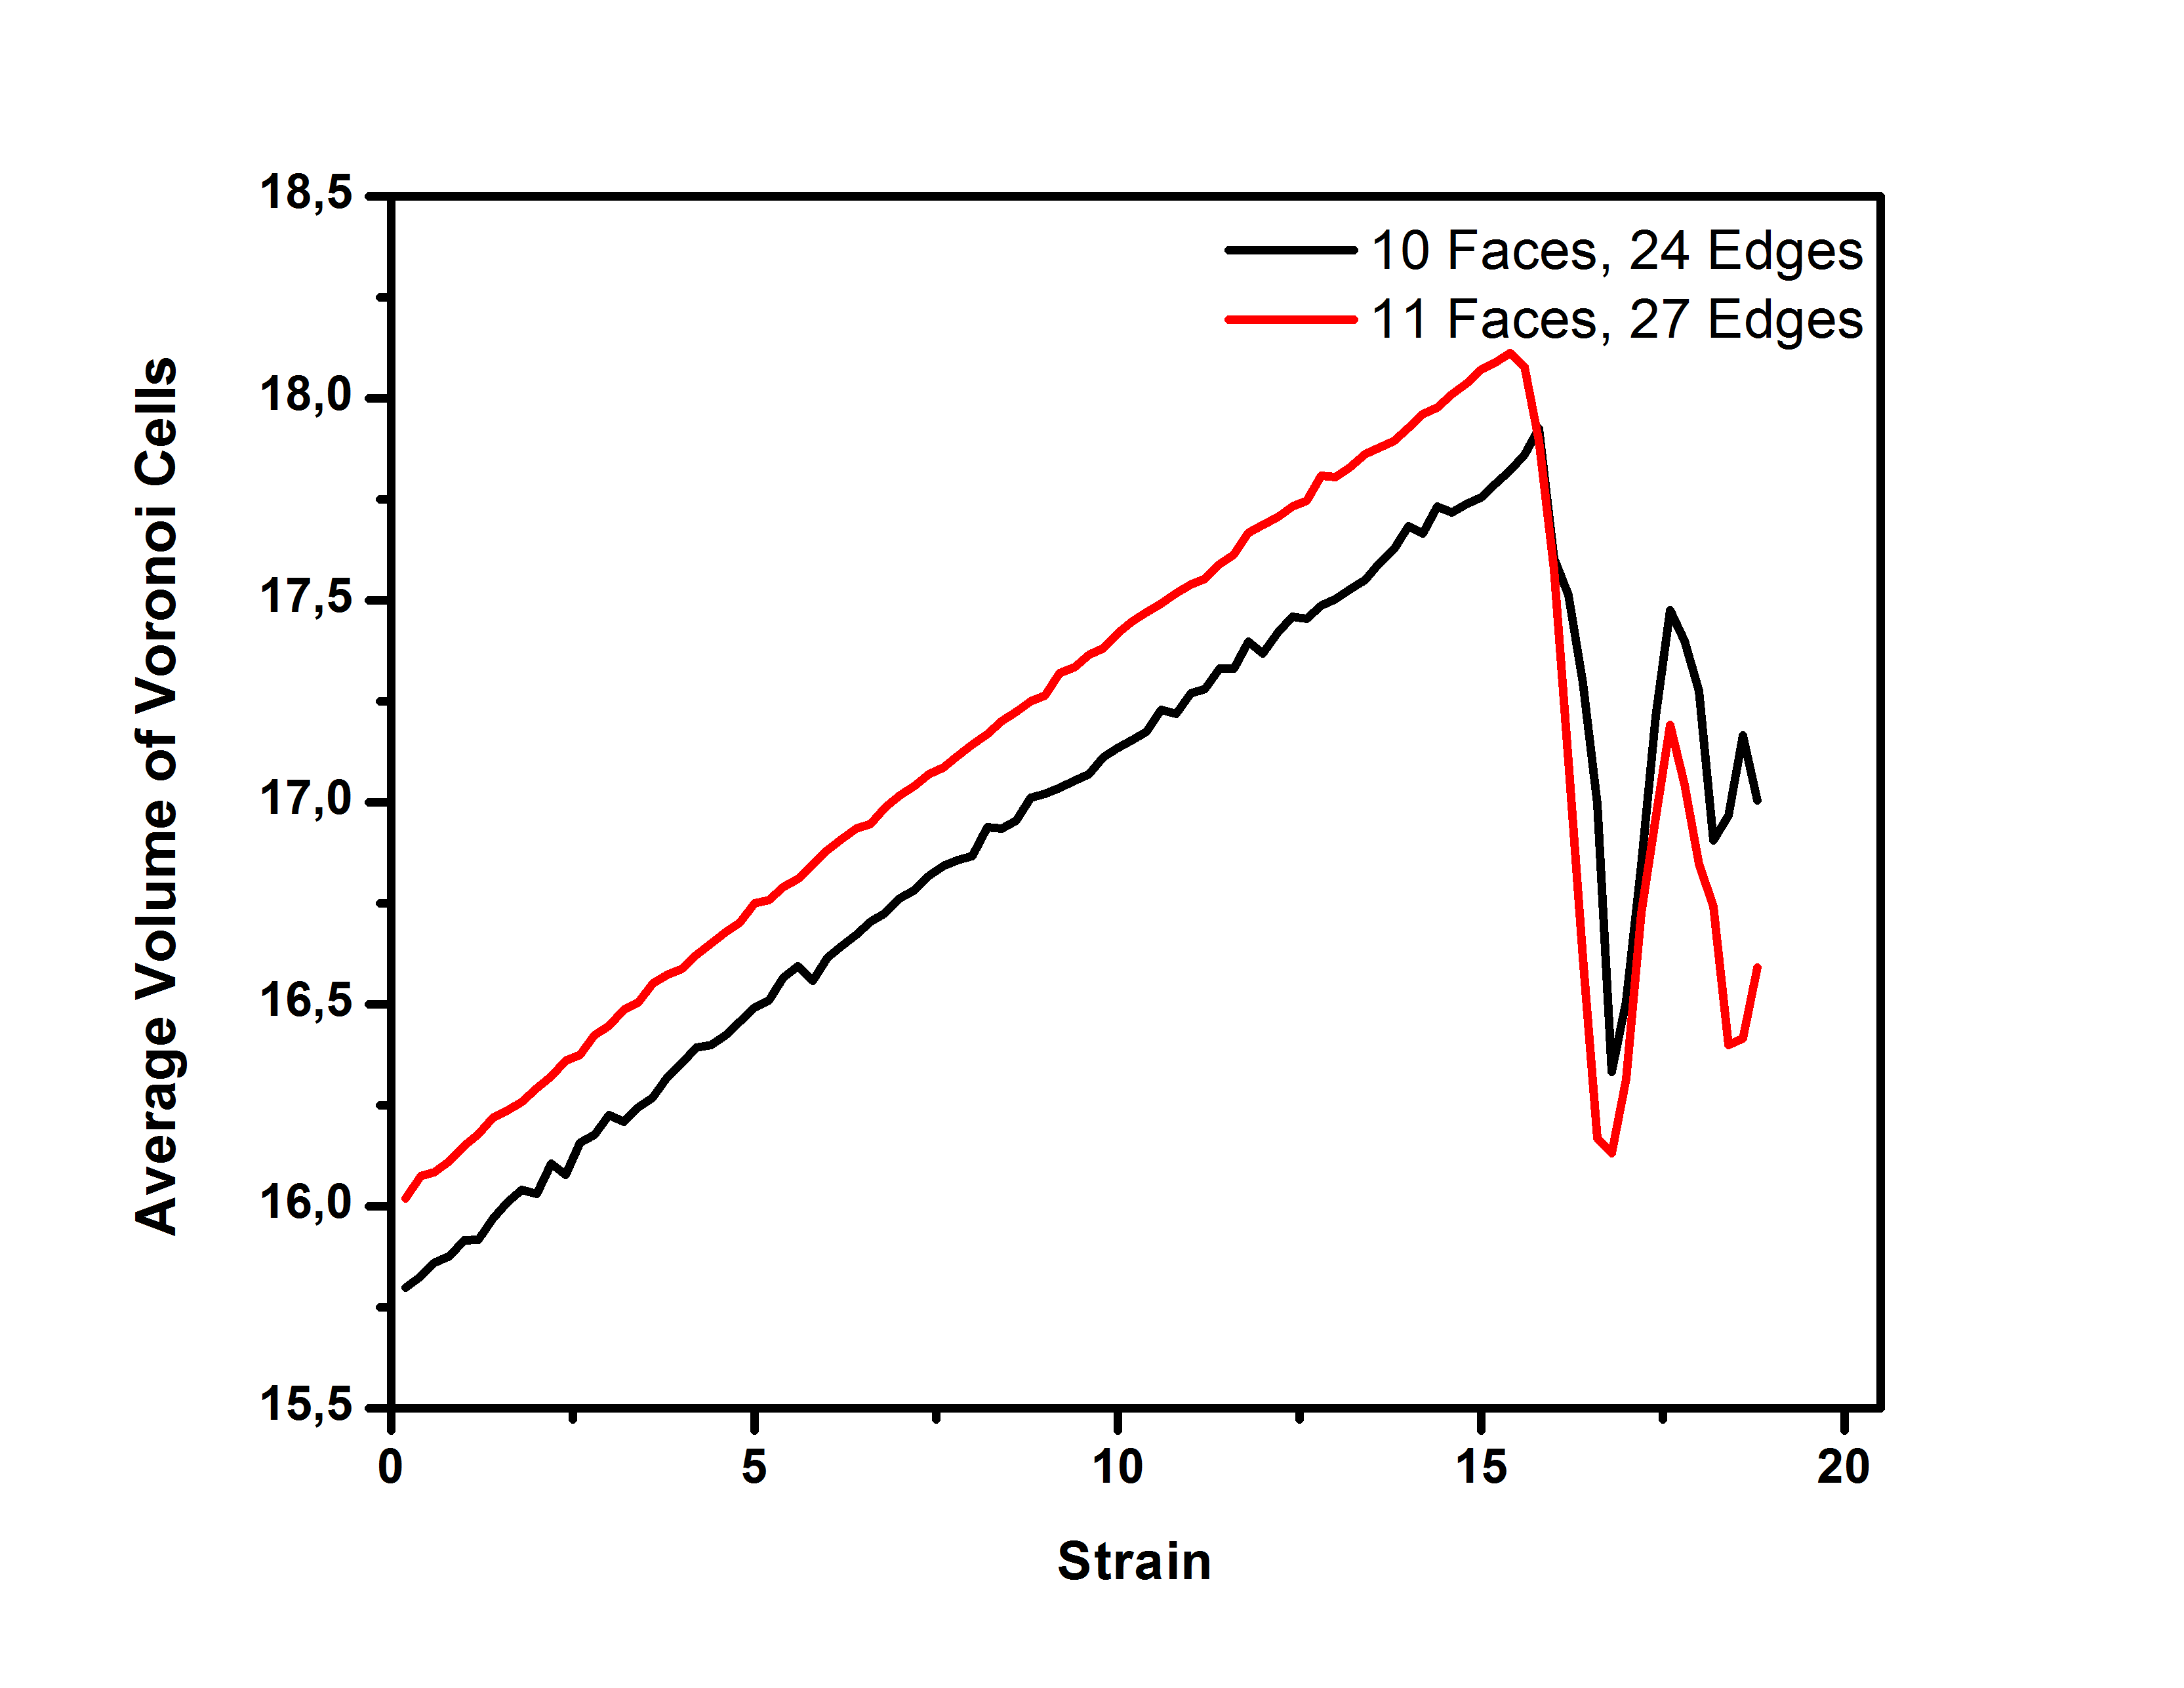
\includegraphics[width=8cm]{Figures/TRAC_Vol_Step_B.png}
\caption{volumen promedio de voronoi cells (parte 2/2, temperatura desconocida)}
\end{figure}

\begin{figure}[H]
\centering
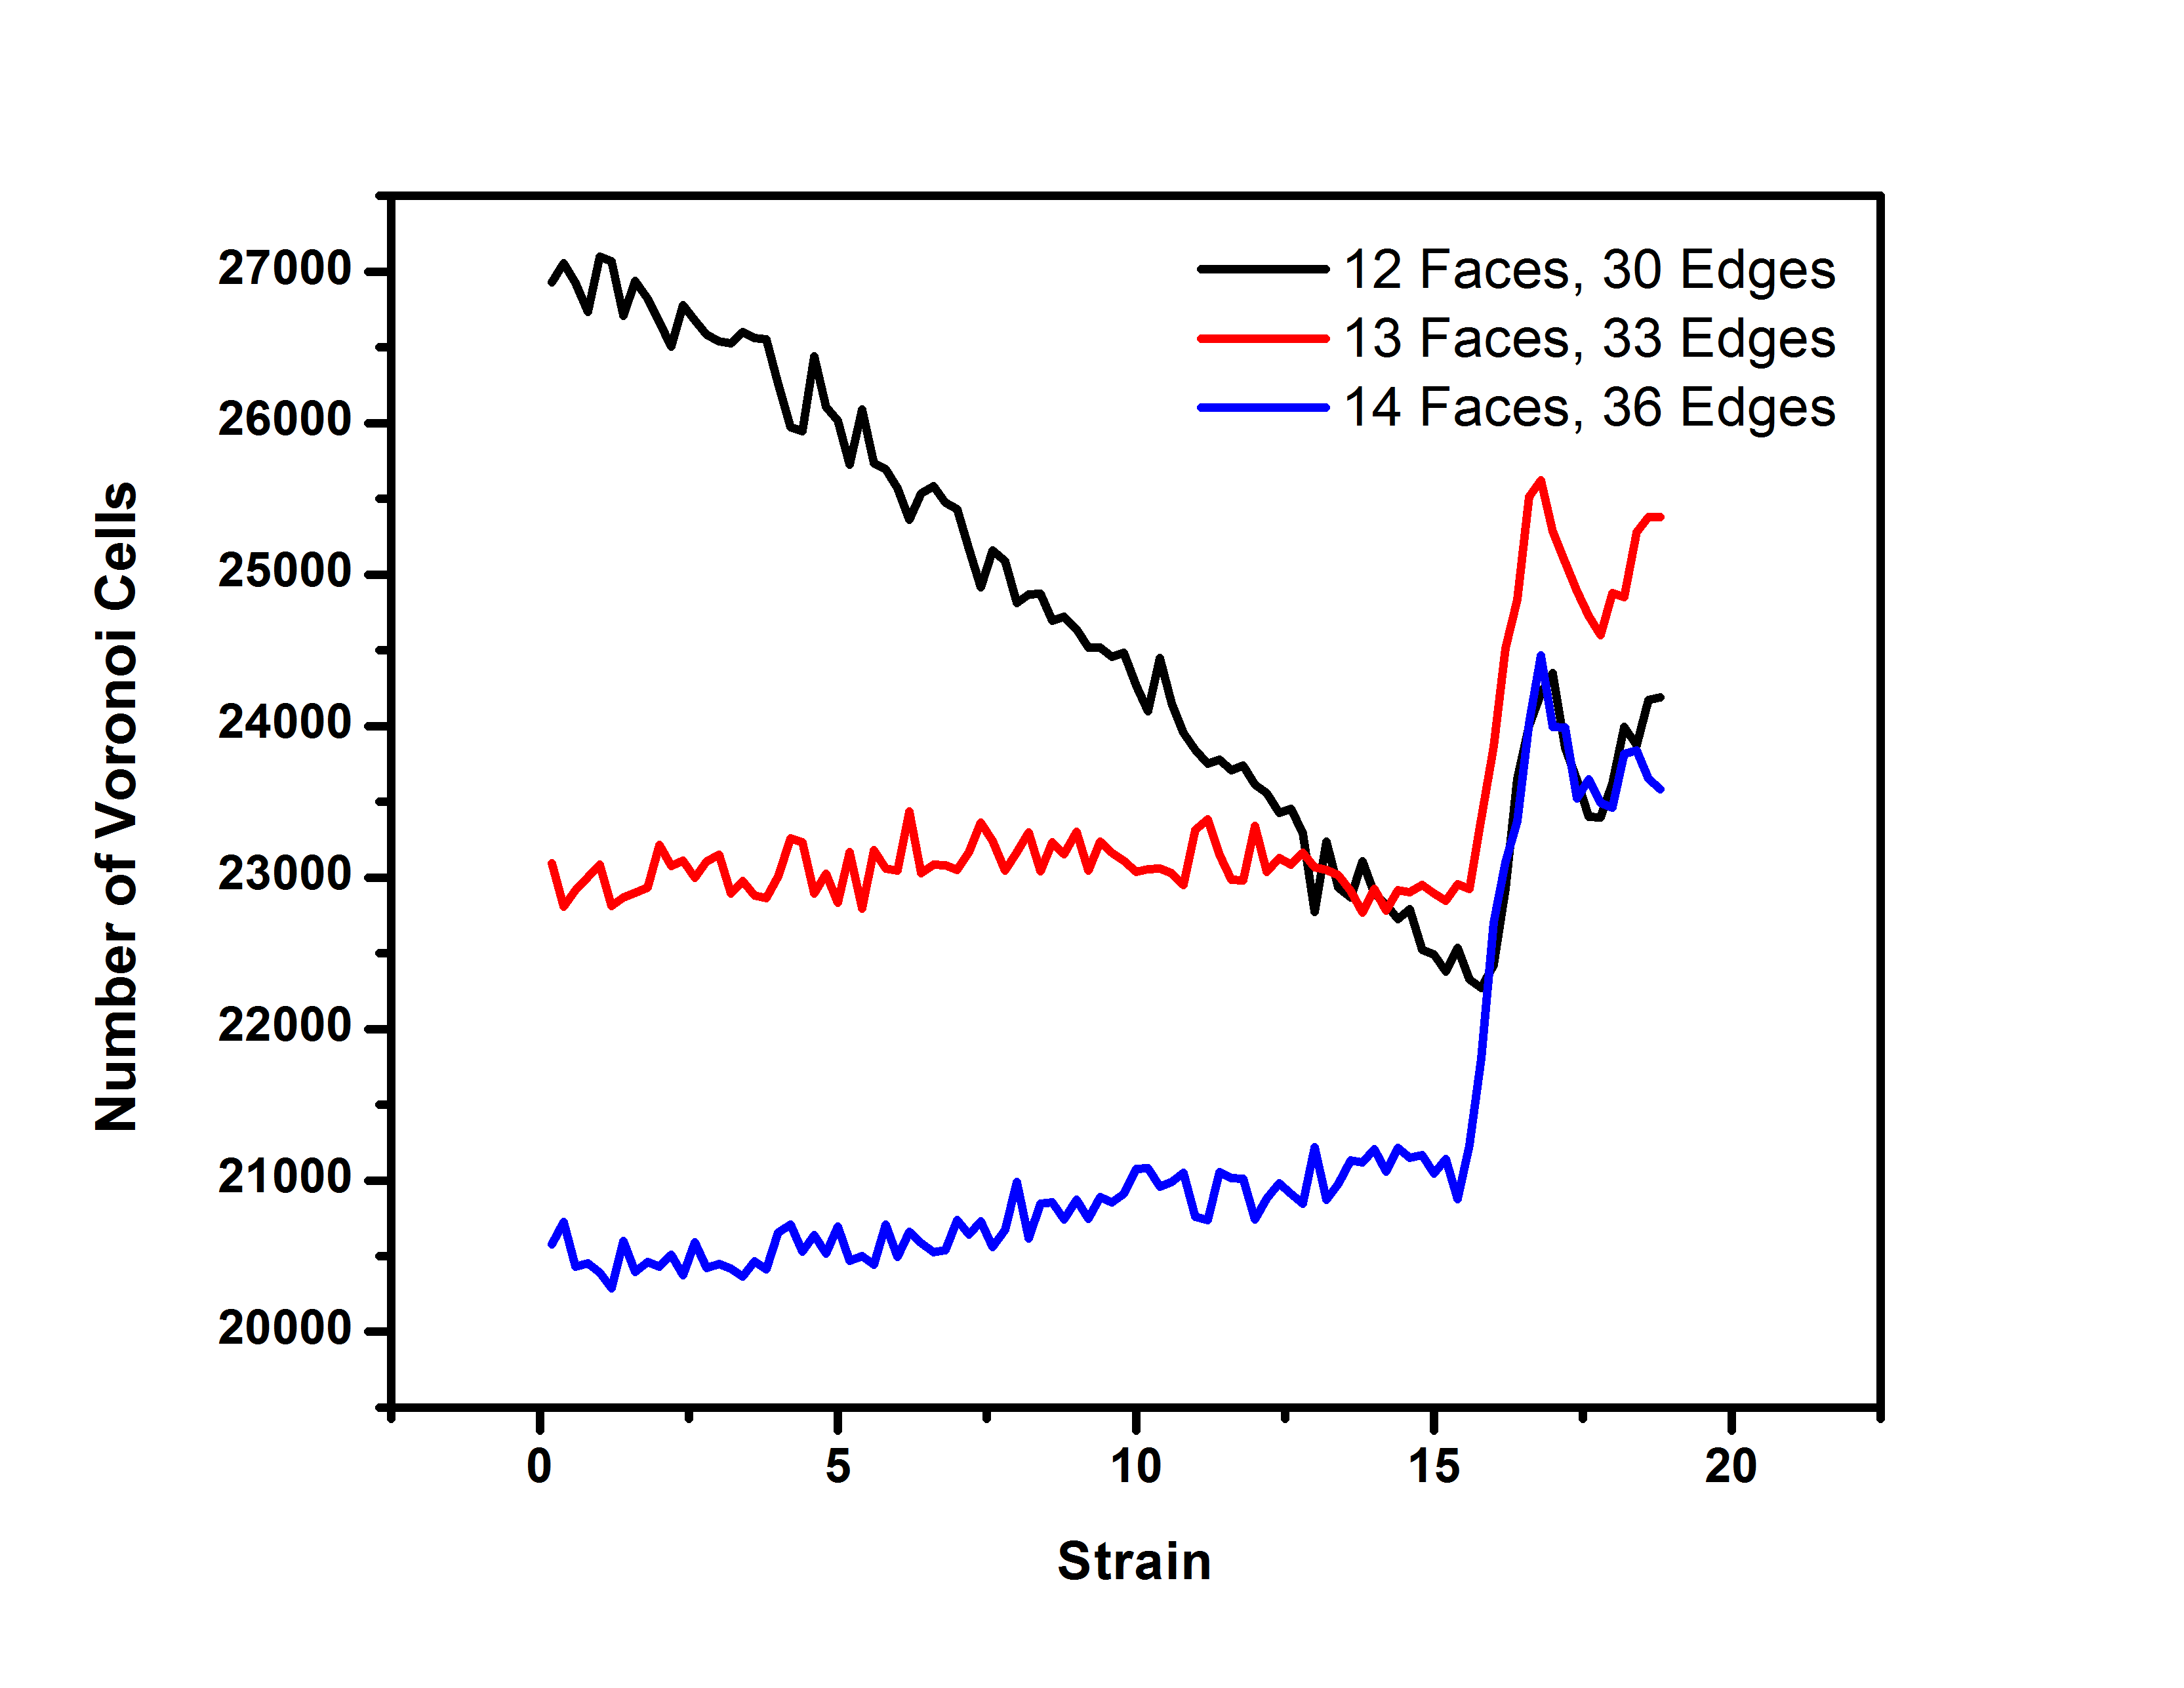
\includegraphics[width=8cm]{Figures/TRAC_Num_Step_B.png}
\caption{numero celdas de voronoi (parte 1/4, temperatura desconocida)}
\end{figure}

\begin{figure}[H]
\centering
\includegraphics[width=8cm]{Figures/TRAC_Num_Step_C.png}
\caption{numero celdas de voronoi (parte 2/4, temperatura desconocida)}
\end{figure}

\begin{figure}[H]
\centering
\includegraphics[width=8cm]{Figures/TRAC_Num_Step_D.png}
\caption{numero celdas de voronoi (parte 3/4, temperatura desconocida)}
\end{figure}

\begin{figure}[H]
\centering
\includegraphics[width=8cm]{Figures/TRAC_Num_Step_E.png}
\caption{numero celdas de voronoi (parte 4/4, temperatura desconocida)}
\end{figure}

%
%	Ambas
%

\subsection{Comparacion}

\begin{figure}[H]
\centering
\includegraphics[width=8cm]{Figures/peakstress_T_BOTH.eps}
\caption{Von Mises maximo vs. Temperatura}
\end{figure}

\begin{figure}[H]
\centering
\includegraphics[width=8cm]{Figures/young_T_both.eps}
\caption{Modulo Young vs. Temperatura}
\end{figure}

\begin{figure}[H]
\centering
\includegraphics[width=8cm]{Figures/defstress_T_BOTH.eps}
\caption{Von Mises a strains vs. Temperatura}
\end{figure}

\end{document}
